\topictitle{Visualisation of Table Datasets}{}

\begin{topicsummary}
    \item This topic explains how to choose visual idioms for tabular data by aligning \textit{What} (data structure), \textit{Why} (task), and \textit{How} (encoding).
    \item It starts with vocabulary clarification (idiom, graph, plot, diagram, chart, map) and then applies a consistent What--Why--How analysis to each chart family.
    \item Core idioms covered are bar charts (including stacked bars and dot-plot alternatives), line and area charts, pie charts, scatterplots, and bubble plots.
    \item For each idiom, the notes provide practical guidance on when to use it, when to avoid it, and how to refine the design for clarity, accuracy, and readability.
    \item The chapter closes with an idiom-selection snapshot table that maps common idioms to their typical data form, analytical purpose, and primary visual encoding.
\end{topicsummary}

\section{Vocabulary}
Before discussing chart choices, we first clarify six terms that are often used interchangeably but are not identical.
\margincitebox[Vocabulary Sources]{kirk2019,munzner2014}

\begin{itemize}
    \item \textbf{Idiom} is a reusable visual design pattern for data. In these notes, words such as chart, plot, and map are treated as specific kinds of idioms.\sidenote{In Munzner's framework, an idiom is the design choice that maps abstract data and tasks to visual form \parencite{munzner2014}}
    \item \textbf{Graph} is a general visual representation of relationships or values. In different contexts, it can refer to a plotted function, a network structure, or a broad class of data graphics.
    \item \textbf{Plot} usually refers to a coordinate-based representation where data is placed against explicit axes and scales. Scatterplots and line plots are typical examples.
    \item \textbf{Diagram} is a schematic representation that emphasises structure, flow, or concept relationships, often without precise quantitative scales.
    \item \textbf{Chart} is a practical data display designed for communication and comparison. Bar charts, line charts, and pie charts are common chart forms.
    \item \textbf{Map} is a spatial representation tied to geographic or geometric location, where position carries meaning through coordinate systems or topology.
\end{itemize}

With these terms defined, we can now discuss how to select and evaluate idioms for tabular datasets in a consistent way.

\section{Idiom: Bar Charts}
\paragraph{Brief}
A bar chart uses rectangular bars to compare values across categories. It is one of the most common comparison charts, and it is often the first choice when the analysis goal is to compare magnitudes clearly.
\marginnotebox{READING LENS}{Read each idiom in three passes: \textbf{What} (data abstraction), \textbf{Why} (task abstraction), and \textbf{How} (idiom, marks, channels, and form).}

\whatpill\  A bar chart uses one \textbf{categorical key attribute} and one \textbf{quantitative value attribute} per \textbf{item}. The key identifies category membership (one bar per category), and the value determines bar length from a common zero baseline.

\begin{figure*}[htbp]
    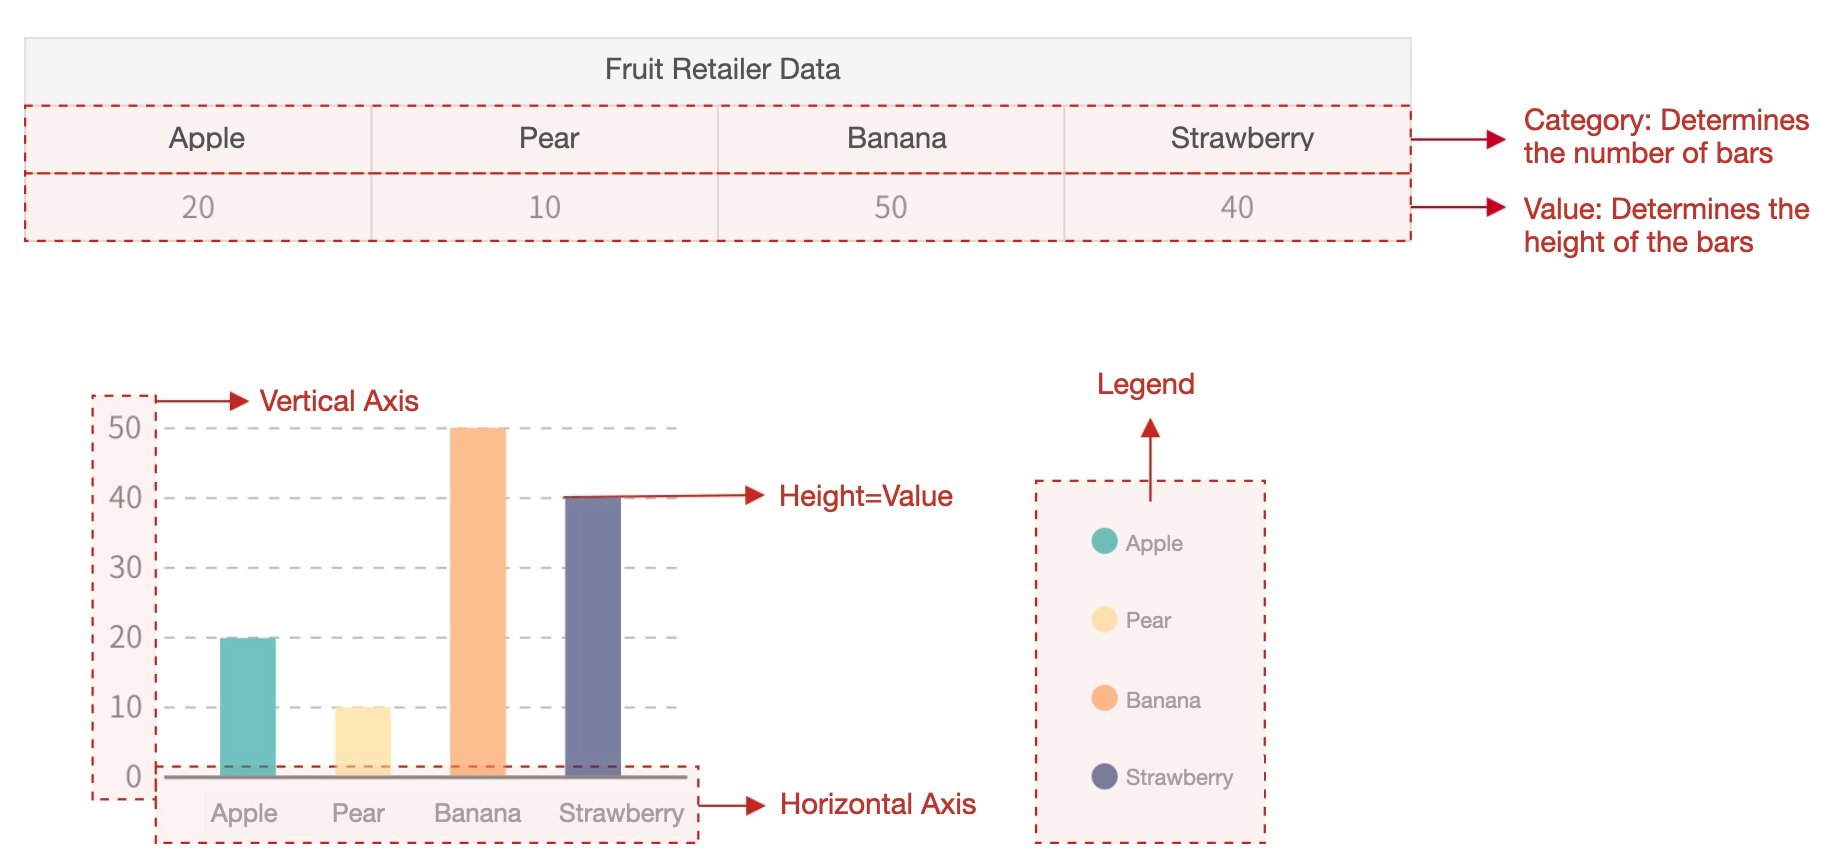
\includegraphics[width=\linewidth]{images/bar-chart/bar-elemental-composition.png}
    \caption{Elemental composition of a bar chart: category determines bar count, value determines bar height.}
    \label{fig:bar-elemental-composition}
\end{figure*}

\whypill\  The dominant \textit{actions} are \textbf{query} (identify, compare, and lookup category values) and \textbf{search} (find maxima, minima, or unusual categories). The main \textit{targets} are categorical groups and their quantitative magnitudes.

\howpill\  At the \textbf{idiom} level, the \textit{mark} is \textbf{line} (drawn as bars). The primary \textit{channels} are \textbf{length} on a common scale for quantitative value and \textbf{spatial region/order} for category identity. This mapping is high in \textbf{effectiveness} for magnitude comparison; practical \textbf{scalability} is usually dozens to hundreds of items.

% \begin{marginfigure}[1.2\baselineskip]
%     \centering
%     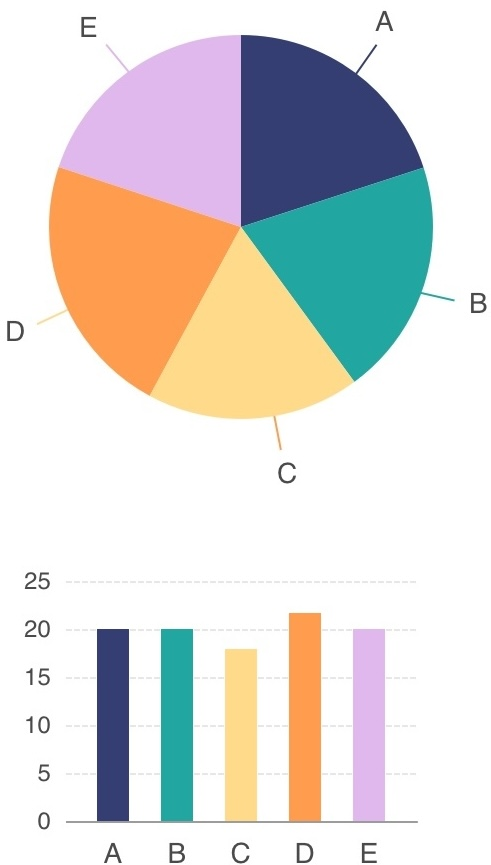
\includegraphics[width=0.92\linewidth]{images/bar-chart/bar-applicable-close-values.jpeg}
%     \caption{A typical scenario where bar charts support clear comparison across categories.}
%     \label{fig:bar-applicable-scenario}
% \end{marginfigure}



\subsection*{Design Guide}
\paragraph{Use when}
\begin{itemize}
    \item \textit{Categorical comparison with close values.} Bar charts are best suited for comparing categorical data, especially when values are close together, because people judge aligned length more accurately than area or angle.~\sidenote{For details on the ranking of visual channels, refer to the course note: \textbf{Mark and Chanel}}
\end{itemize}


\begin{marginfigure}
    \centering
    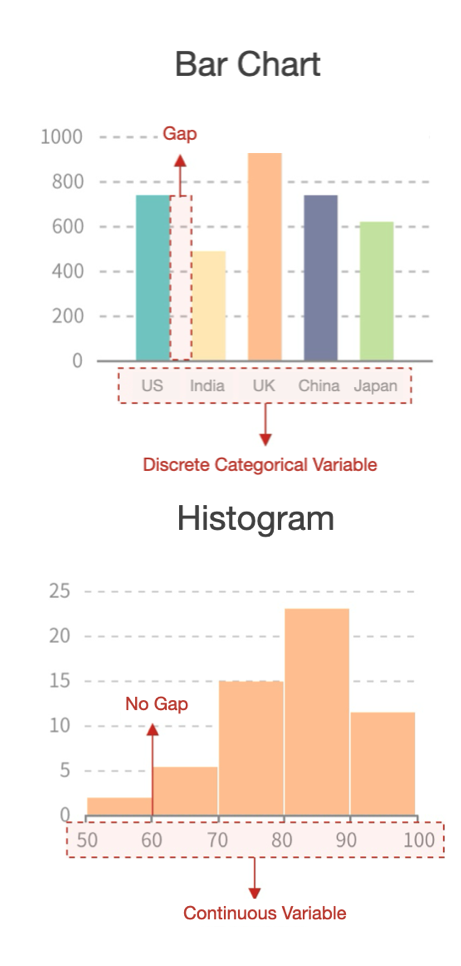
\includegraphics[width=\textwidth]{images/bar-chart/bar-vs-histogram-discrete-vs-continuous.png}
    \caption{Discrete-category bar chart versus continuous-bin histogram semantics.}
    \label{fig:bar-inapplicable-histogram}
    \vspace{6pt}
\end{marginfigure}

\paragraph{Avoid when}

\begin{itemize}
    \item \textit{Continuous data distribution.} Bar charts require discrete categories and visible gaps between bars. If the data is continuous, a histogram is the correct idiom because bins are continuous intervals (see Figure~\ref{fig:bar-inapplicable-histogram}).
    \item \textit{Truncated baseline manipulation.} The core function of a bar chart is comparison through length. If the y-axis does not start at zero, proportional judgement becomes distorted and the visual difference no longer matches the numerical difference.
\end{itemize}

\begin{figure}[htp]
    \centering
    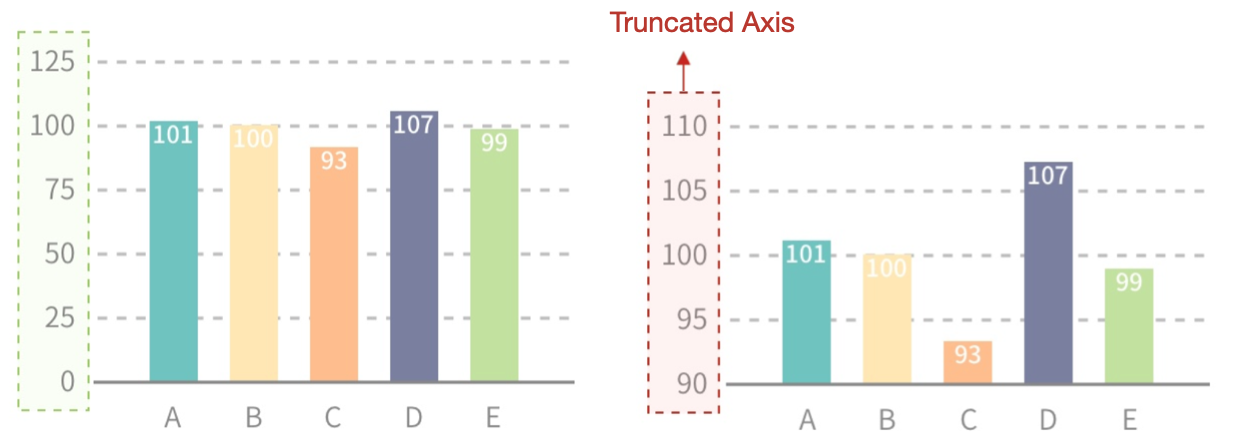
\includegraphics[width=\linewidth]{images//bar-chart/bar-truncated-axis-misleading.png}
    \caption{Axis truncation exaggerates differences. Left: a bar chart with a zero baseline shows true relative differences. Right: truncating the vertical axis visually amplifies small variations, potentially misleading interpretation.}
    \label{fig:bar-truncated-axis-misleading}
\end{figure}


As shown in Figure~\ref{fig:bar-truncated-axis-misleading}, truncating the baseline can exaggerate visual gaps that do not match the underlying numbers. This is not only a style preference. Research shows that truncated bar/column axes lead to strong overestimation of differences. In a controlled 2015 study, participants who saw deceptive charts interpreted the exaggerated message more strongly \parencite{pandey2015deceptive, datawrapper_bar_baseline_guidance}.

\begin{marginfigure}
    \centering
    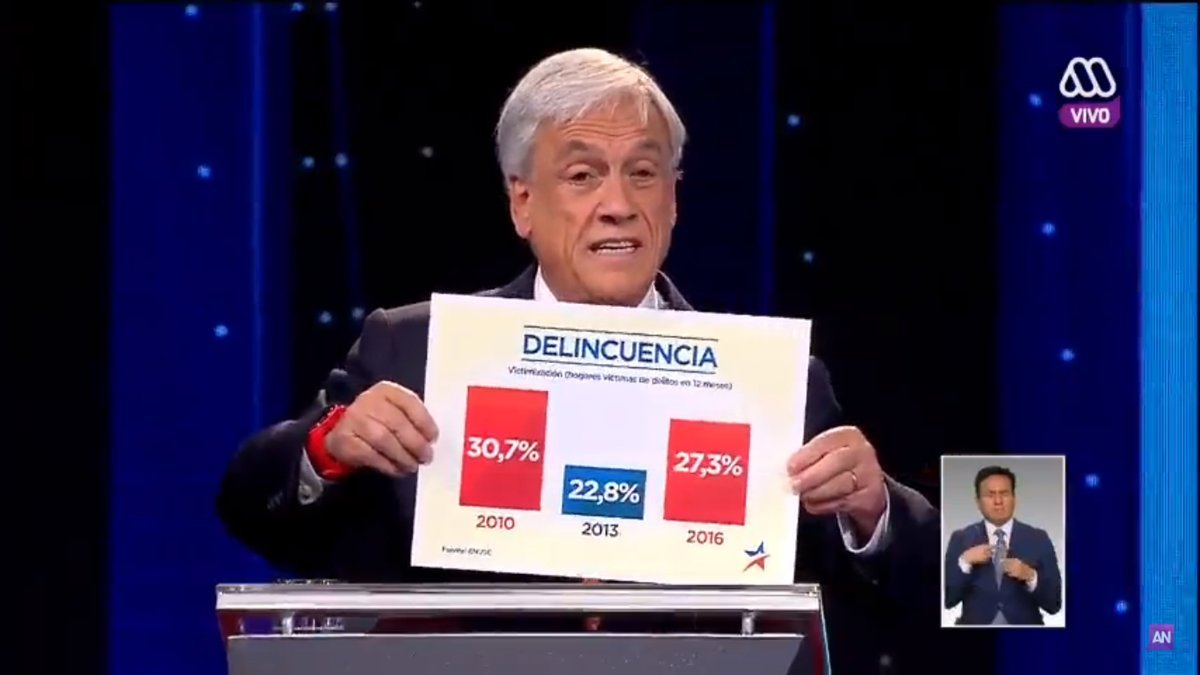
\includegraphics[width=\linewidth]{images/bar-chart/truncated-baseline-pinera-campaign.jpeg}
    \caption{A example is a campaign chart presented by former Chilean president Sebasti\'an Pi\~nera, where a 4.5\% gap appeared visually similar to a much larger 22.8\% gap, while a 3.4\% gap looked disproportionately small. Such distortions illustrate why bar charts must preserve a zero baseline to maintain proportional length comparison.}
    \label{fig:bar-baseline-pinera}
\end{marginfigure}

%\paragraph{Wrap up}
In summary, bar charts are powerful for categorical comparison but require careful design to avoid misleading interpretations. The key refinement suggestions are: 

\paragraph{Refinements}
\begin{figure*}[htbp]
    \centering
    \begin{minipage}[t]{0.48\linewidth}
        \centering
        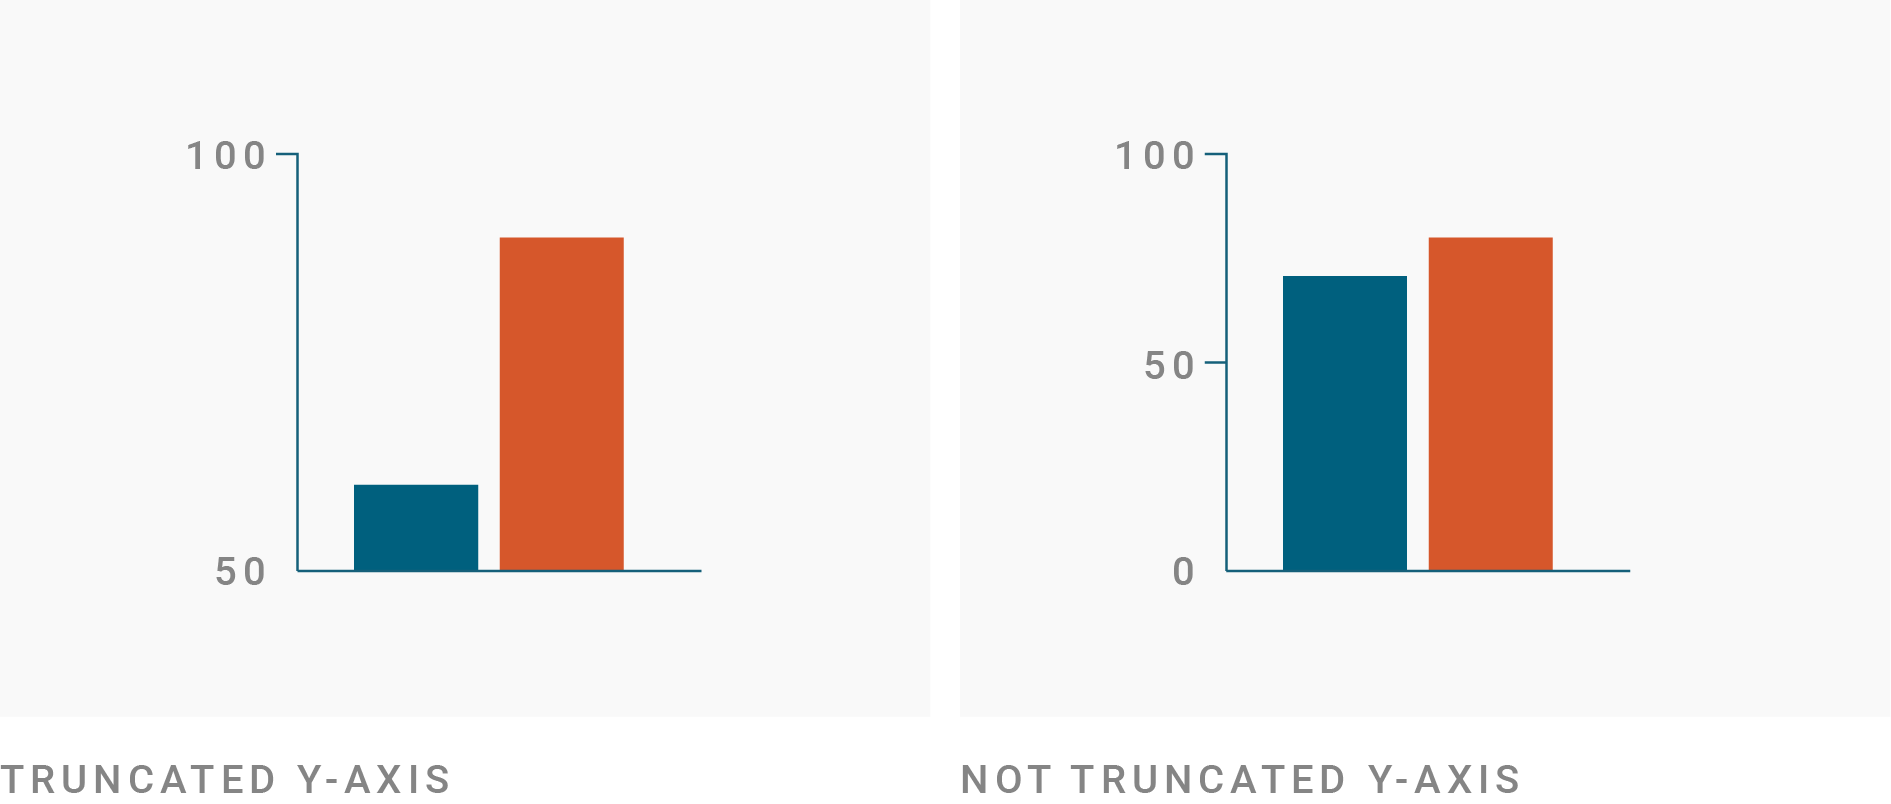
\includegraphics[width=\linewidth]{images/bar-chart/truncated-baseline-deceptive-comparison.png}
        \fullwidthfigurecaption{Always compare a truncated bar chart with a zero-baseline version before publishing; if the message changes, the truncated view is likely exaggerating differences.}
        \label{fig:baseline-refinement-truncated}
        \label{fig:baseline-refinement-bars-dot}
    \end{minipage}
    \hfill
    \begin{minipage}[t]{0.48\linewidth}
        \centering
        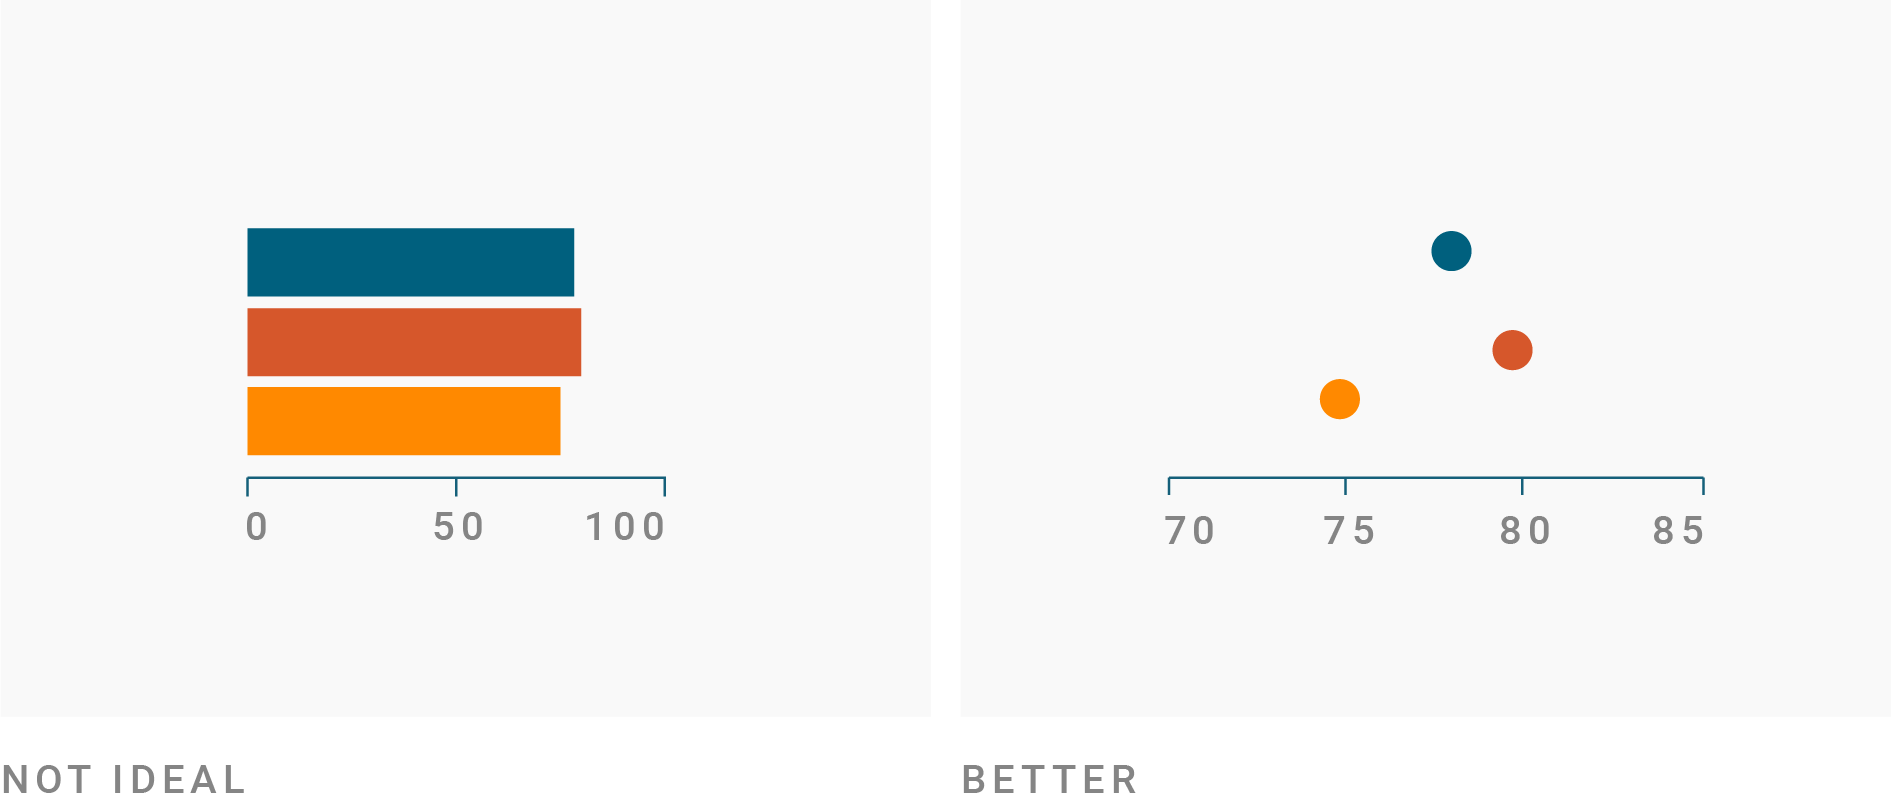
\includegraphics[width=\linewidth]{images/bar-chart/truncated-baseline-alternative-dot-plot.png}
        \fullwidthfigurecaption{Dot plots are better when values are close because aligned position supports finer comparison with less non-data ink than bars.}
        \label{fig:baseline-refinement-dot-plot}
    \end{minipage}
\end{figure*}


\begin{figure*}[htbp]
    \centering
    \begin{minipage}[t]{0.48\linewidth}
        \centering
        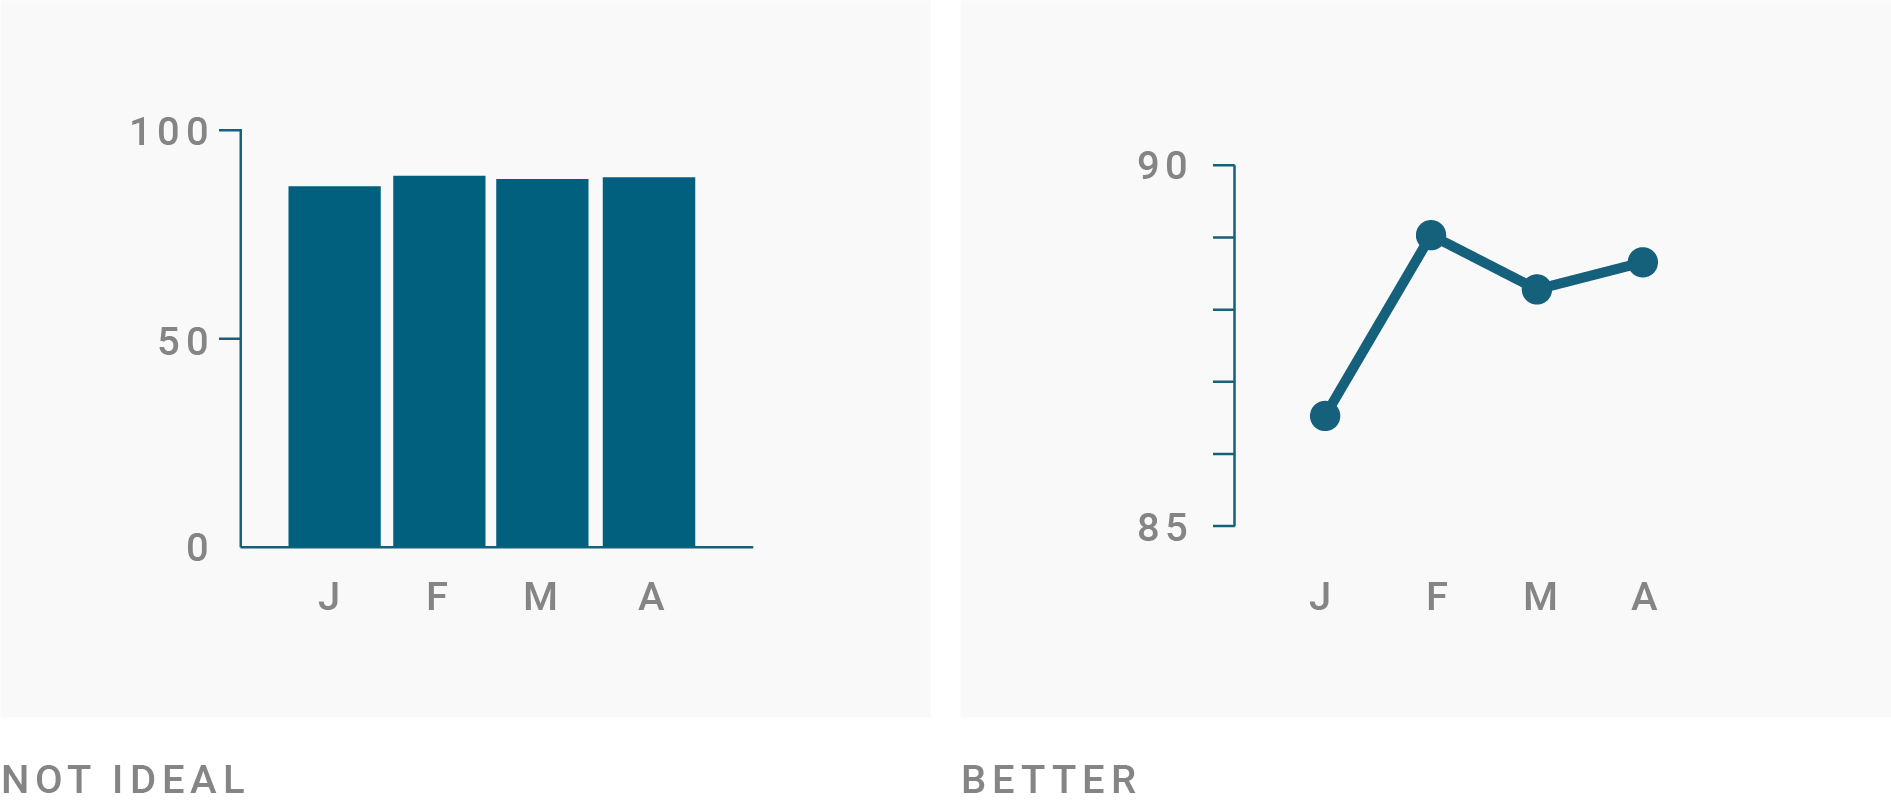
\includegraphics[width=\linewidth]{images/bar-chart/truncated-baseline-alternative-line-chart.png}
        \fullwidthfigurecaption{Line charts are preferable for ordered categories such as months or years, where direction and rate of change matter more than isolated magnitudes.}
        \label{fig:baseline-refinement-line-chart}
        \label{fig:baseline-refinement-line-diff}
    \end{minipage}
    \hfill
    \begin{minipage}[t]{0.48\linewidth}
        \centering
        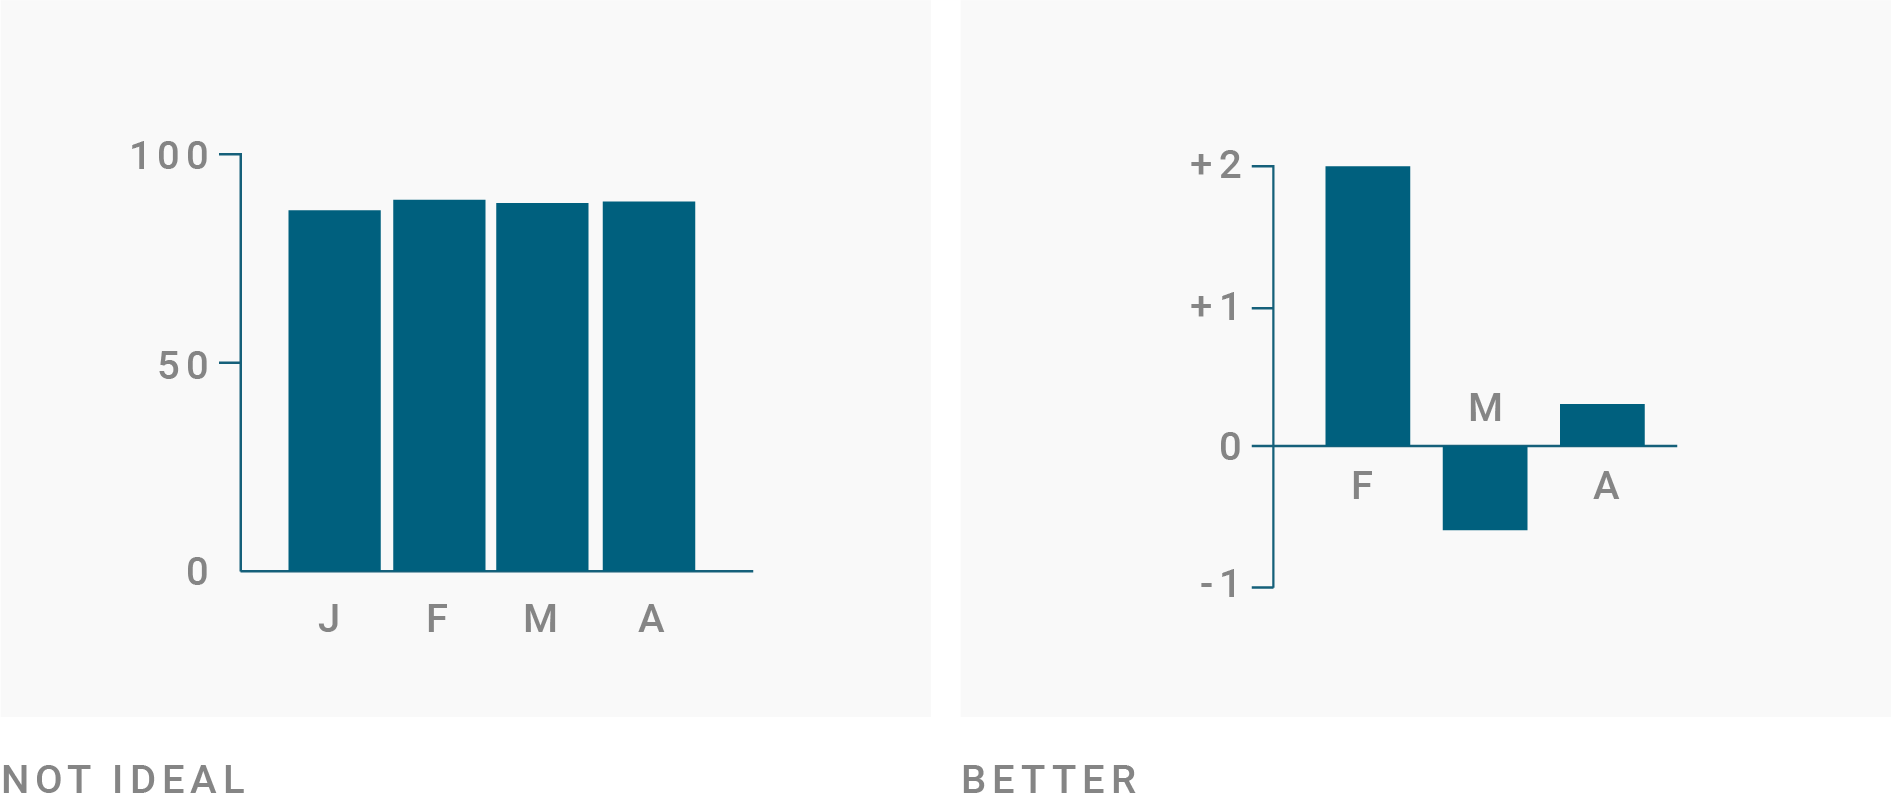
\includegraphics[width=\linewidth]{images/bar-chart/truncated-baseline-alternative-differences.png}
        \fullwidthfigurecaption{Difference charts encode adjacent deltas directly, making small increases and decreases readable without relying on visual subtraction between bars.}
        \label{fig:baseline-refinement-difference-chart}
    \end{minipage}
\end{figure*}

Bar charts form a family of related idioms. A simple bar chart supports direct comparison across categories; a grouped bar chart enables comparison between subgroups; a stacked bar chart combines totals with composition; and a 100\% stacked bar chart emphasises relative composition rather than absolute totals. In a 100\% stacked chart, all bars have equal length, so absolute values are intentionally suppressed. In the following section, we discuss when to use stacked bar charts, when a dot plot may be a better alternative, and when these designs should be avoided.

\subsection{Stacked Bar Chart}
\paragraph{Brief}
A stacked column chart, also called a stacked bar chart, is used to break a whole into parts while preserving category totals. Compared with a simple bar chart, each category bar is divided into multiple subcategories, usually distinguished by color.
\margincitebox[Stacked Bar References]{datawrapper_stacked_column_charts}

\whatpill\  Stacked bars add one extra \textbf{categorical key attribute}: one key defines each bar, the second key defines the internal segment category, and one \textbf{quantitative value attribute} defines segment size.

\begin{figure*}[htbp]
    \centering
    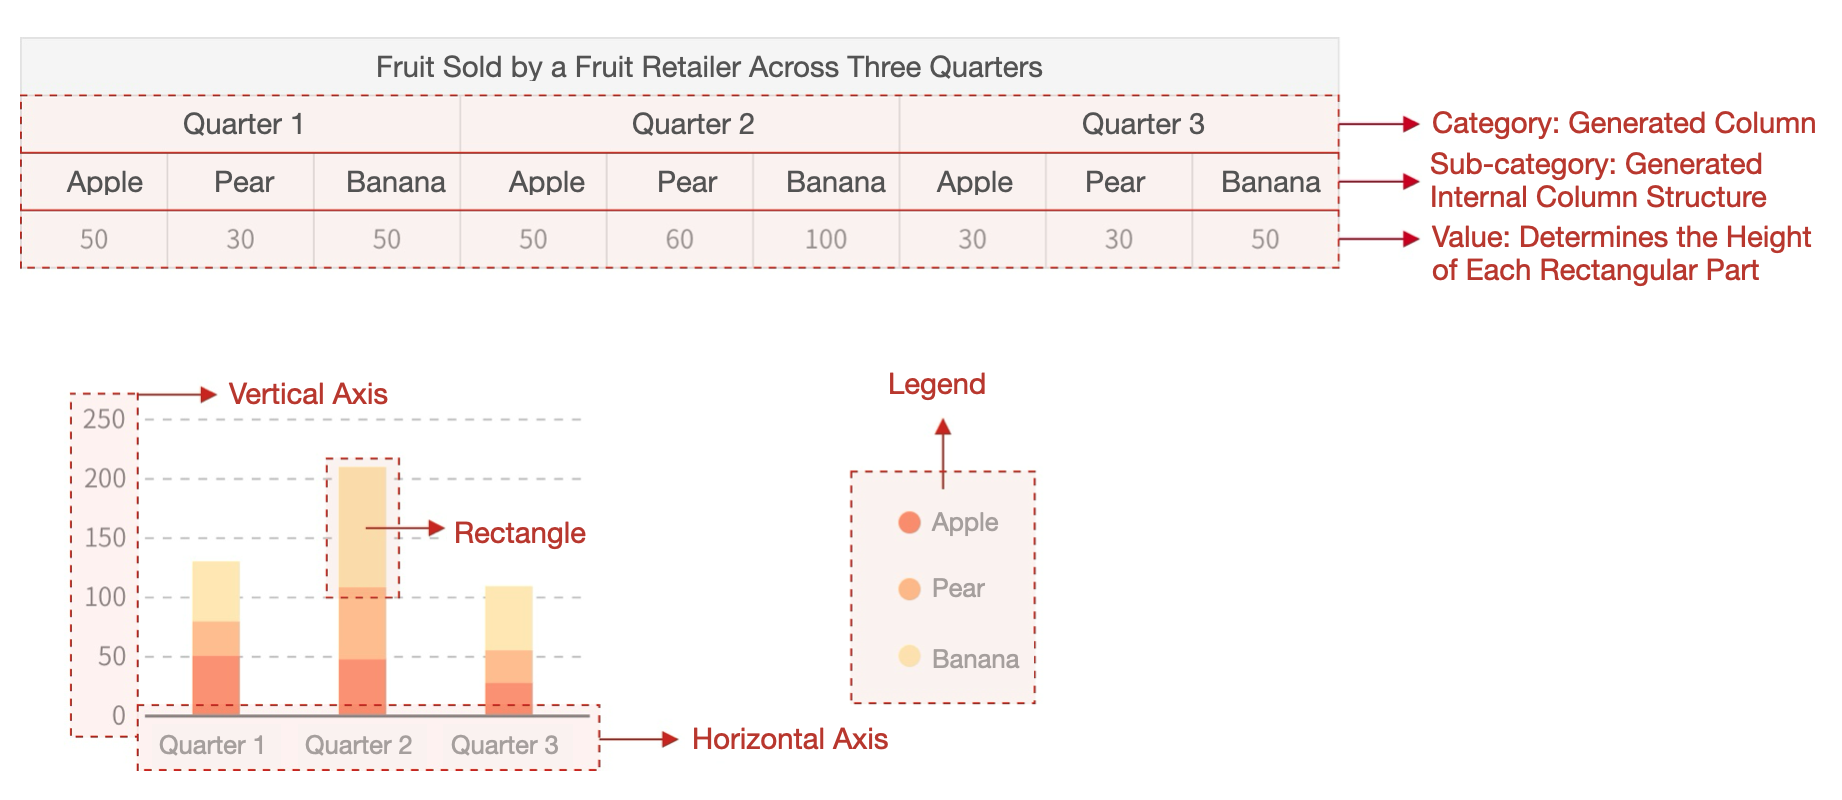
\includegraphics[width=0.92\linewidth]{images/bar-chart/stacked-bar-elemental-composition.png}
    \caption{Elemental composition of a stacked bar chart.}
    \label{fig:stacked-bar-elements}
\end{figure*}

\whypill\  The main \textit{actions} are \textbf{query} (totals and component shares) and \textbf{compare} (composition across categories). The primary \textit{target} is a \textbf{part-to-whole relationship} together with total magnitude.

\howpill\  At the \textbf{idiom} level, the chart is a \textbf{composite glyph} built from stacked line segments; the base \textit{mark} is \textbf{line}. The main \textit{channels} are segment \textbf{length} for value, \textbf{hue} for segment category, and \textbf{spatial region/order} for bar identity. \textbf{Scalability} is moderate; too many stacked levels reduce readability.

\subsection*{Design Guide}
\paragraph{Use when}
\begin{itemize}
    \item \textit{Totals and composition matter together.} Stacked bars are effective when both total comparison and part-to-whole relationships are important, and when the number of categories and segments remains manageable.
    \item \textit{Ordered categories with composition.} When the primary key is ordered (for example, time) and we want to show how composition changes across that order, stacked bars can be useful if the number of segments is not too large.
    \item \textit{Relative shares are more important than absolute totals.} In this case, 100\% stacked bars can highlight composition without emphasizing total size.
    \item \textit{Short labels and compact category sets.} Stacked bars work better when labels fit naturally below each column and when the number of categories is not too large.
\end{itemize}

\paragraph{Avoid when}
\begin{itemize}
    \item \textit{Precise part-to-part comparison across many totals.} Most segments do not share a common baseline, so exact comparison is hard. If this is the primary task, use grouped bars, split bars, small multiples, or dot plots.
    \item \textit{Uneven temporal intervals or crossover stories.} If one share overtakes another, line charts often communicate the crossover more clearly. If intervals are irregular, line/area charts represent temporal spacing more faithfully.
    \item \textit{Only one total or one share.} For one total, a simple bar chart usually uses space better; for one share, direct text can be clearer than a chart.
\end{itemize}

%\paragraph{Wrap up}
%In summary, stacked bars can show totals and composition together, but they require careful design to avoid confusion. The key refinement suggestions are:

\paragraph{Refinements}
\begin{figure*}[htbp]
    \centering
    \begin{minipage}[t]{0.48\linewidth}
        \centering
        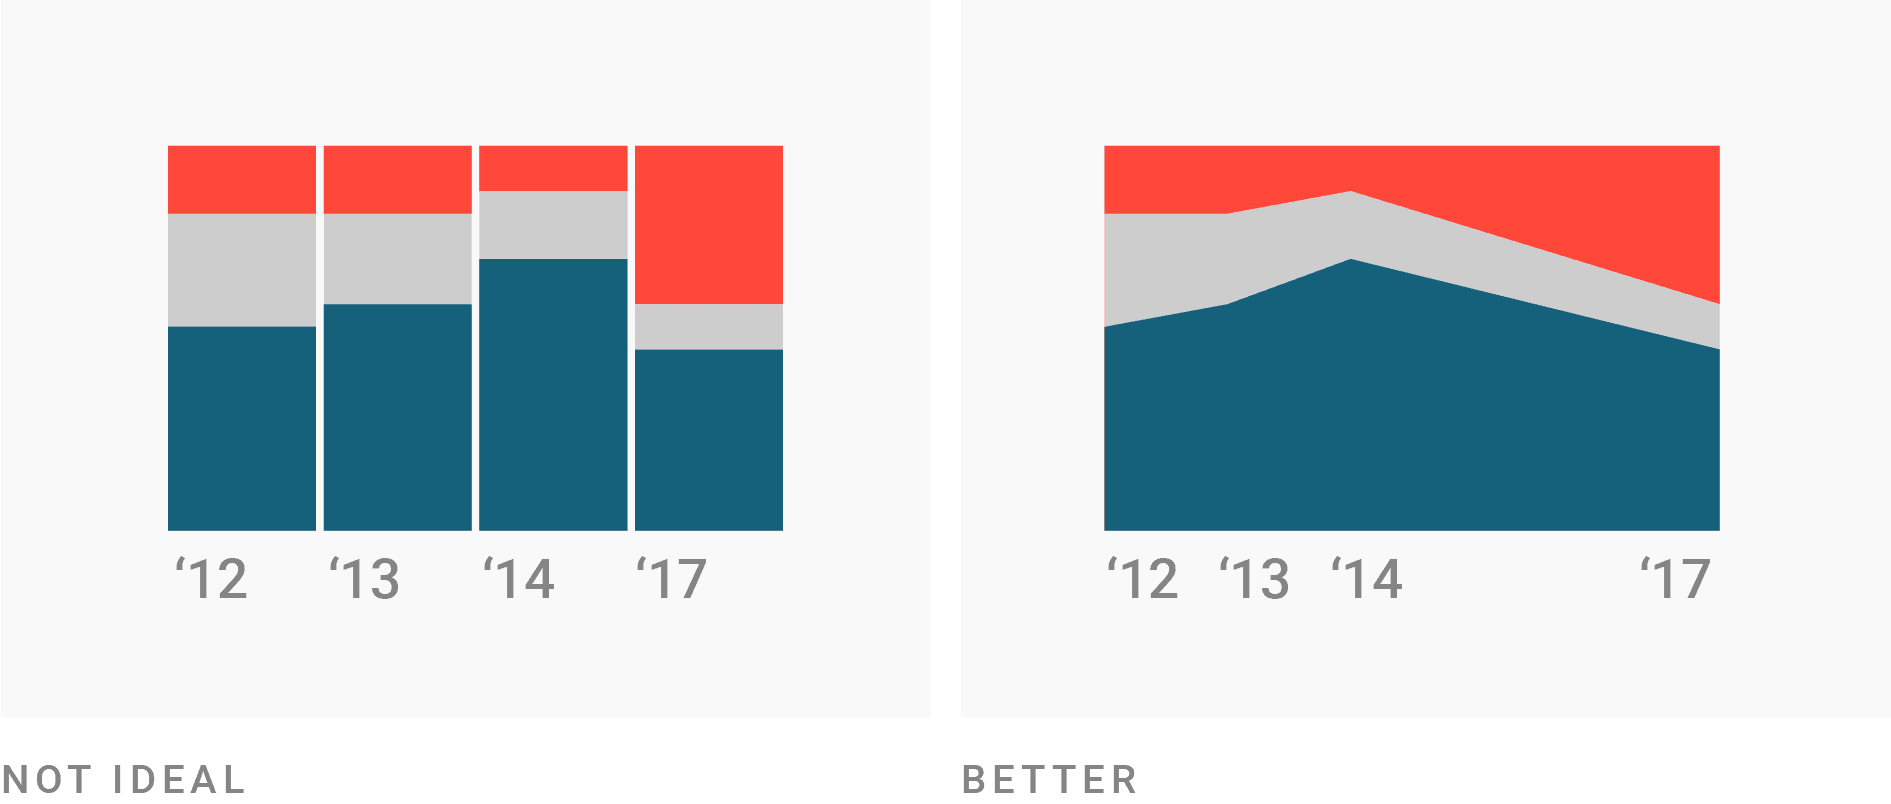
\includegraphics[width=\linewidth]{images/bar-chart/stacked-column-guidance-37-equal-intervals.png}
        \fullwidthfigurecaption{For time data, use stacked columns only when intervals are equal and the number of dates is limited; otherwise line or area charts better preserve temporal spacing.}
        \label{fig:stacked-bar-usage-b}
        \label{fig:stacked-bar-usage-b-equal-intervals}
    \end{minipage}
    \hfill
    \begin{minipage}[t]{0.48\linewidth}
        \centering
        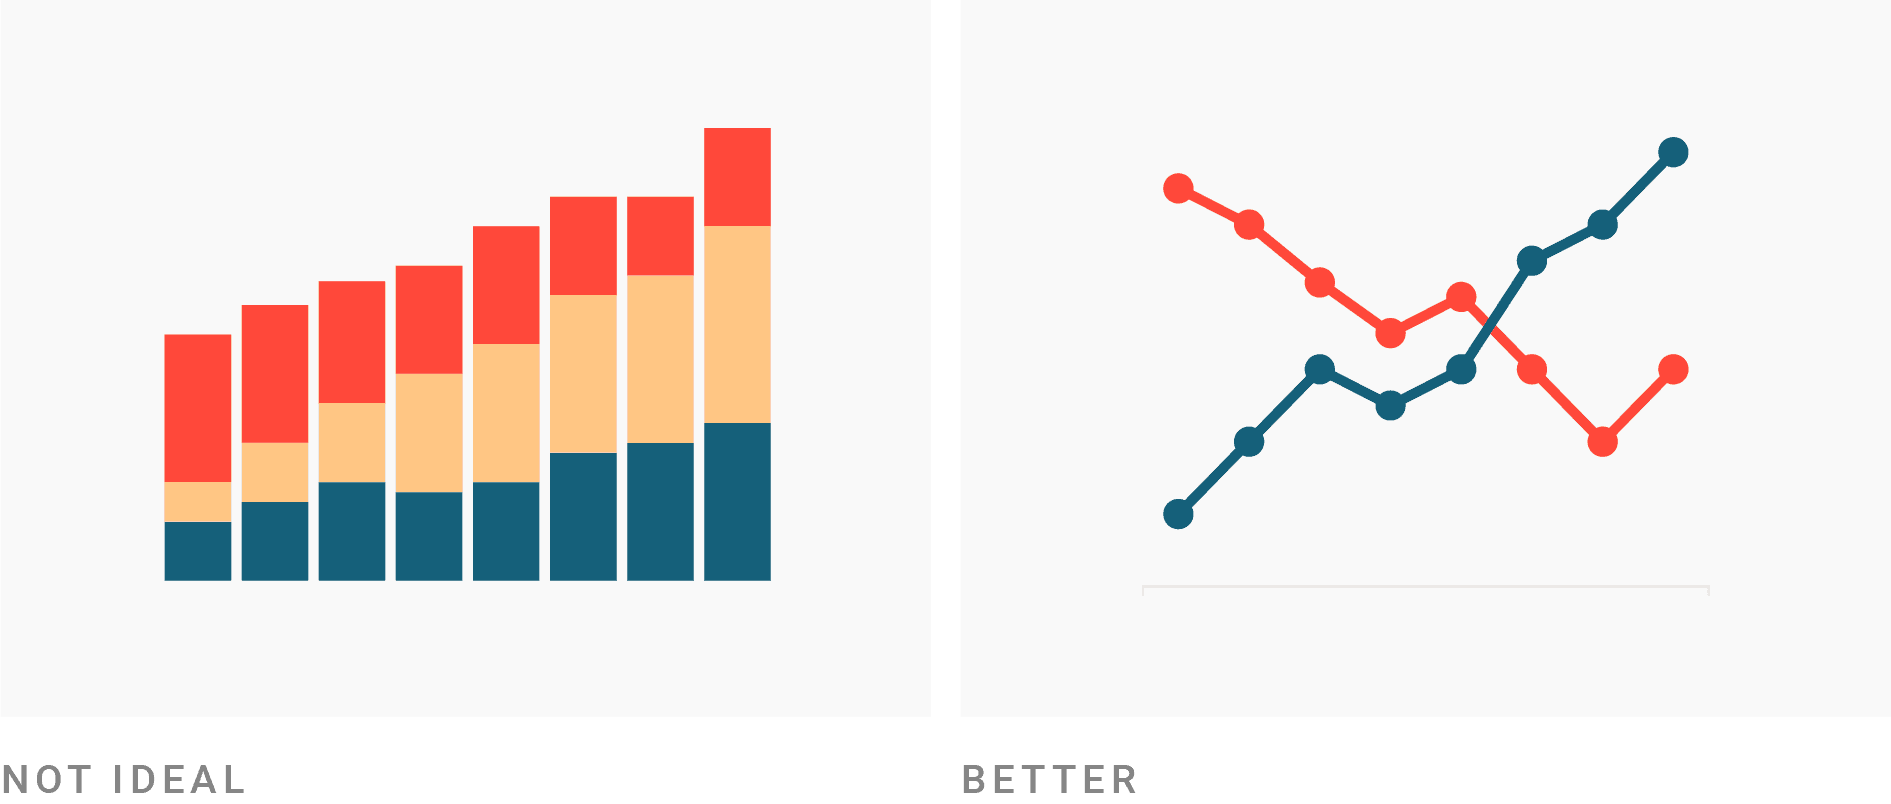
\includegraphics[width=\linewidth]{images/bar-chart/stacked-column-guidance-38-overtake-line.png}
        \fullwidthfigurecaption{When the message is that one share overtook another, switch to a line chart so the crossover is immediately visible and fewer series can be shown.}
        \label{fig:stacked-bar-usage-b-crossover-line}
    \end{minipage}
\end{figure*}

\begin{figure*}[htbp]
    \centering
%    \begin{minipage}[t]{0.48\linewidth}
%        \centering
%        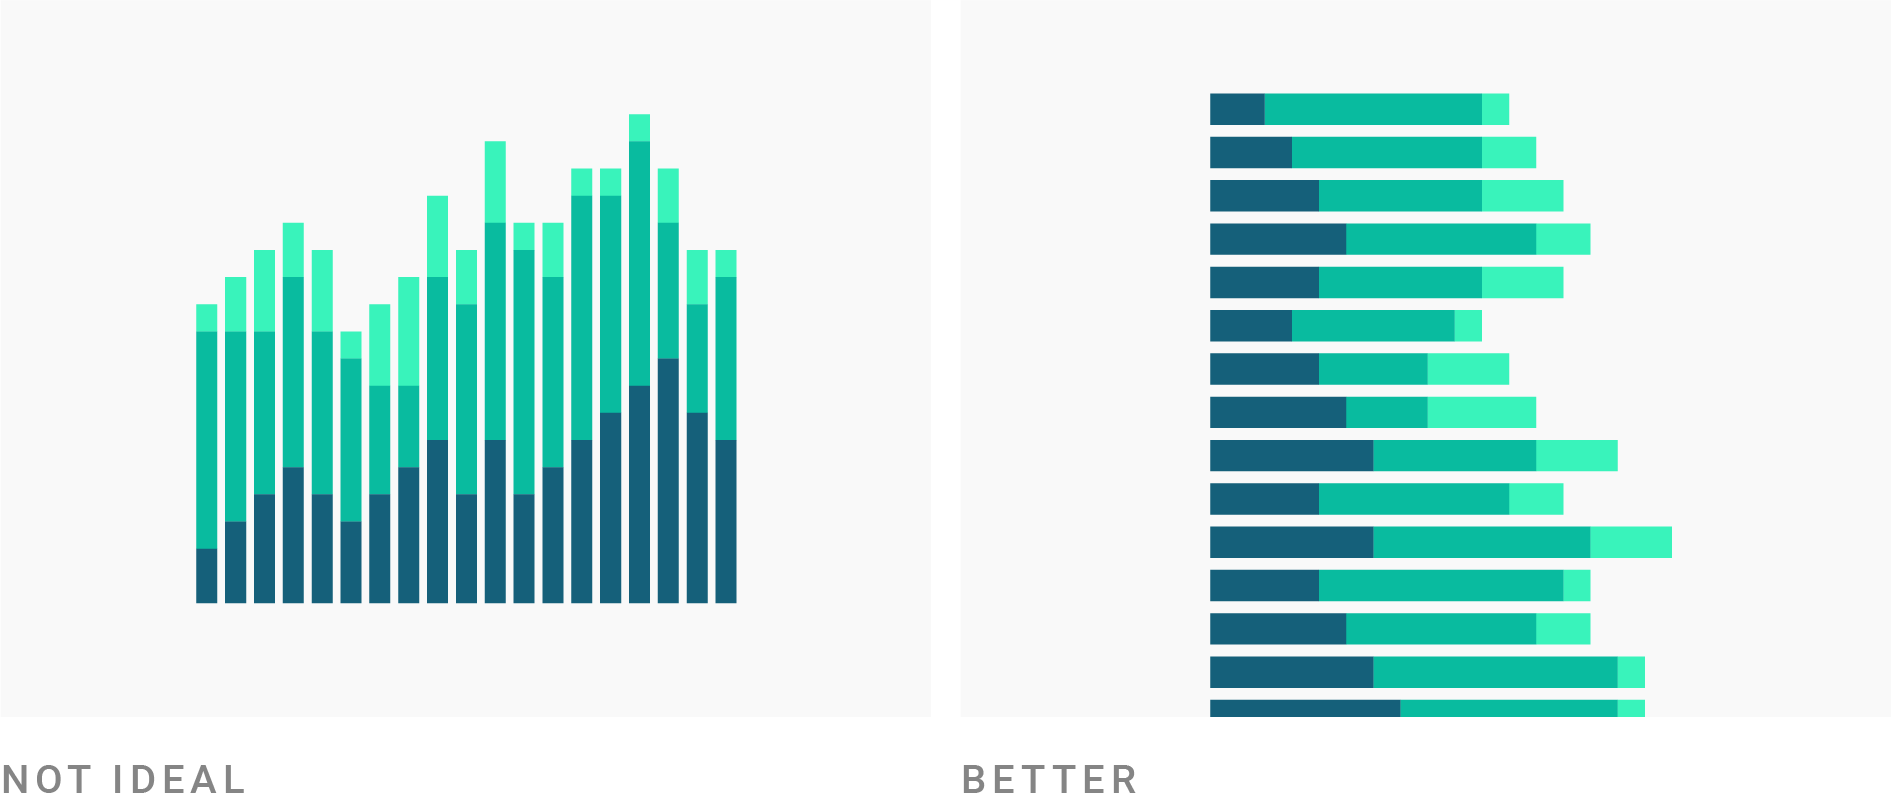
\includegraphics[width=\linewidth]{images/bar-chart/stacked-column-guidance-41-few-totals}
%        \fullwidthfigurecaption{Stacked columns work best for only a few totals; once categories become numerous, limited horizontal space causes crowding and weakens comparison.}
%        \label{fig:stacked-bar-usage-c}
%        \label{fig:stacked-bar-usage-c-many-totals}
%    \end{minipage}
    \begin{minipage}[t]{0.48\linewidth}
        \centering
        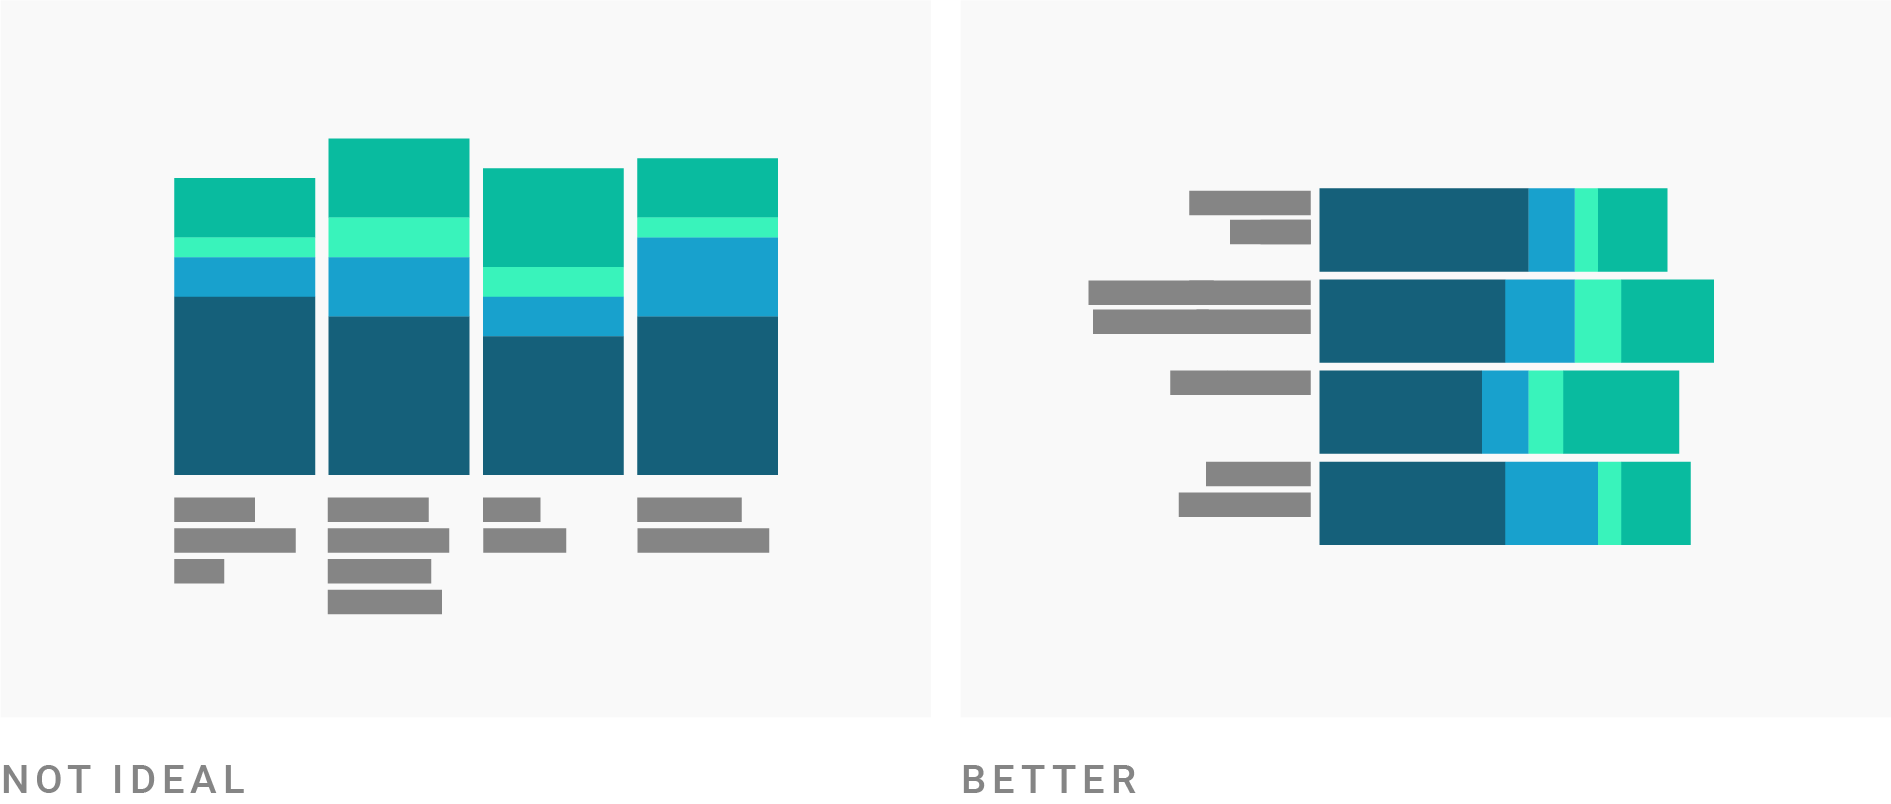
\includegraphics[width=\linewidth]{images/bar-chart/stacked-column-guidance-36-short-labels.png}
        \fullwidthfigurecaption{Keep category labels short in stacked columns; long labels quickly reduce legibility and often indicate that a horizontal stacked bar layout may fit better.}
        \label{fig:stacked-bar-usage-c-short-labels}
    \end{minipage}
\end{figure*}

\begin{figure*}[htbp]
    \centering
    \begin{minipage}[t]{0.48\linewidth}
        \centering
        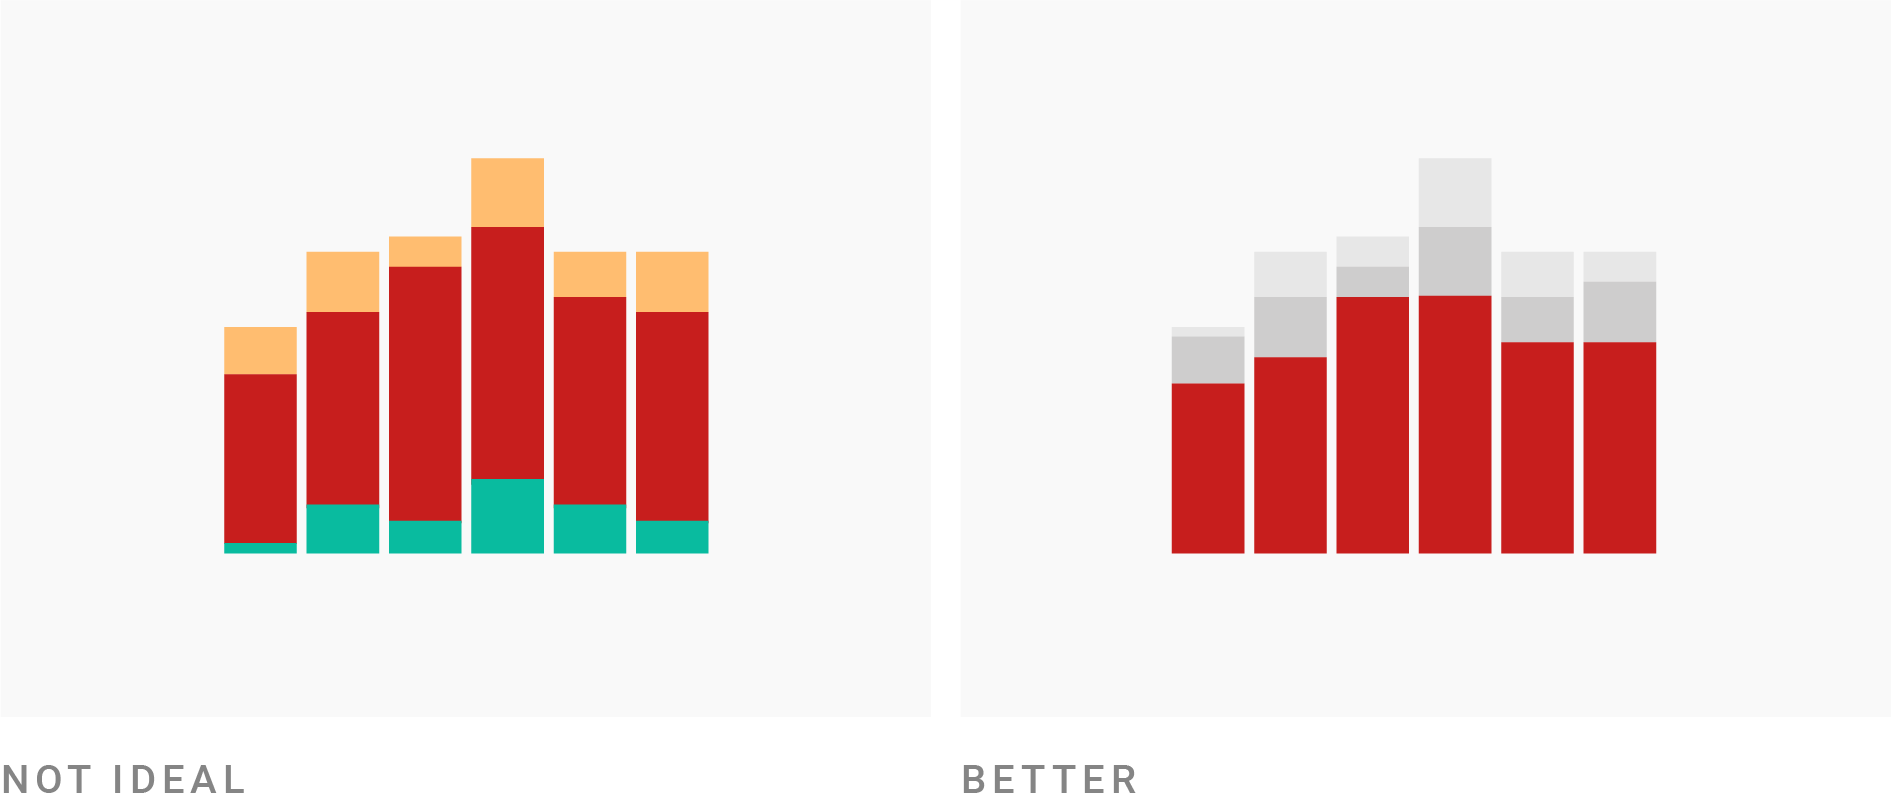
\includegraphics[width=\linewidth]{images/bar-chart/stacked-column-refinement-42-important-bottom.png}
        \fullwidthfigurecaption{Place the most important segment at the baseline and highlight it with stronger color so readers can compare that segment against a shared zero reference.}
        \label{fig:stacked-bar-refinement-a}
        \label{fig:stacked-bar-refinement-a-important-bottom}
    \end{minipage}
    \hfill
    \begin{minipage}[t]{0.48\linewidth}
        \centering
        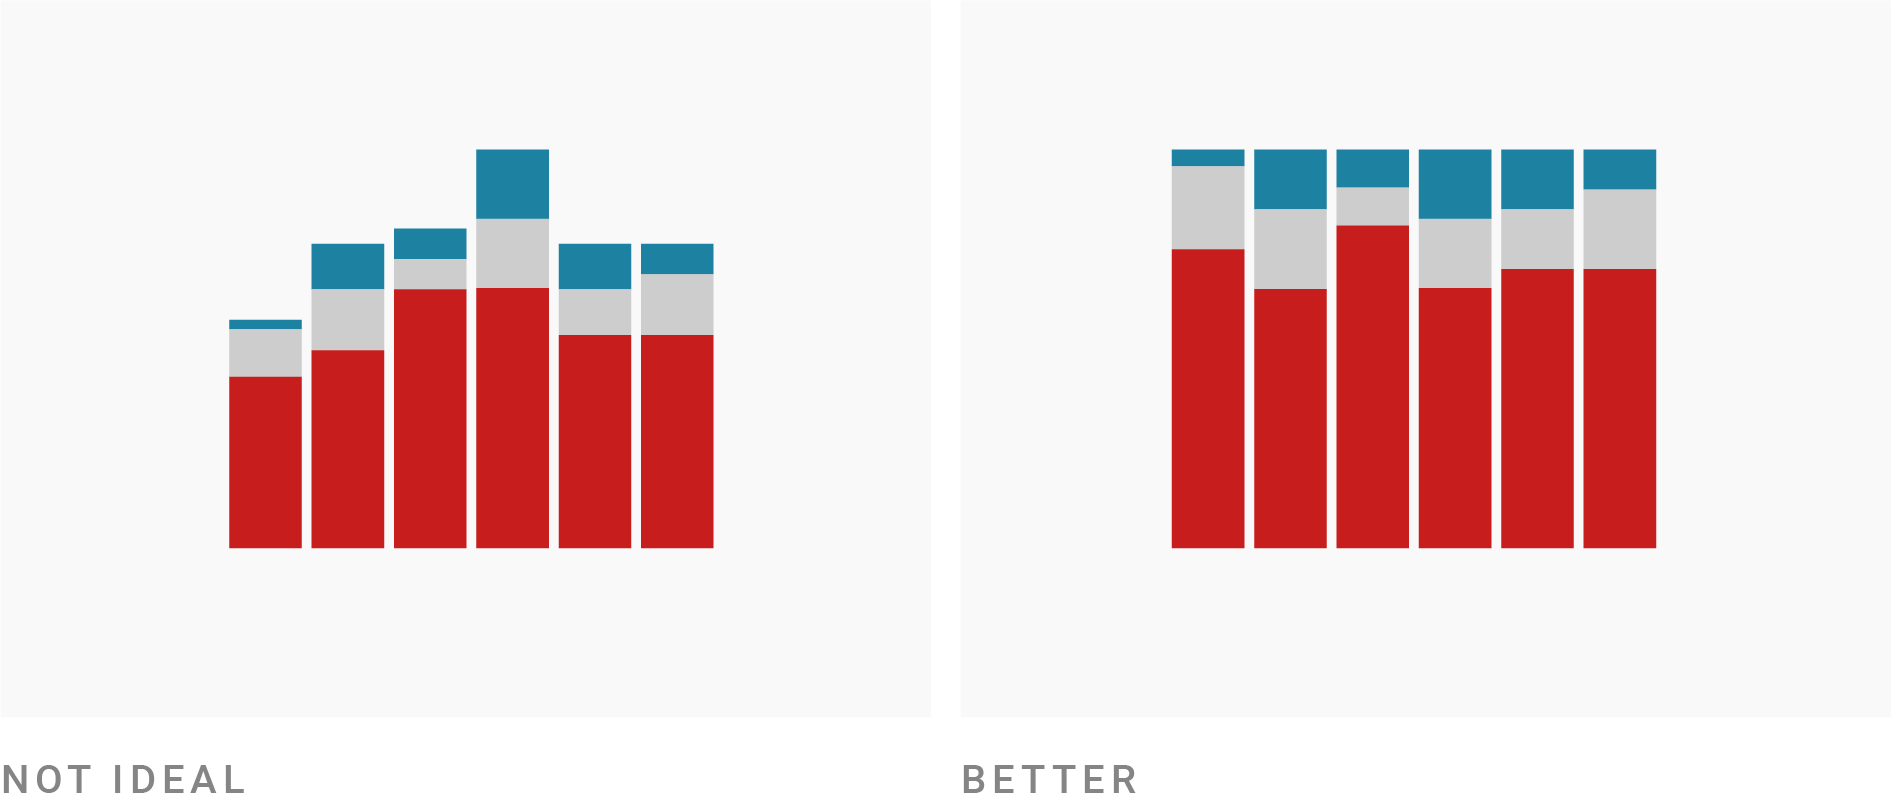
\includegraphics[width=\linewidth]{images/bar-chart/stacked-column-refinement-44-percent-stacking.png}
        \fullwidthfigurecaption{Use 100\% stacking when relative composition matters more than absolute totals; this normalizes bars and adds a clear top baseline for share comparison.}
        \label{fig:stacked-bar-refinement-a-percent-stacking}
    \end{minipage}
\end{figure*}

\begin{figure*}[htbp]
    \centering
    \begin{minipage}[t]{0.48\linewidth}
        \centering
        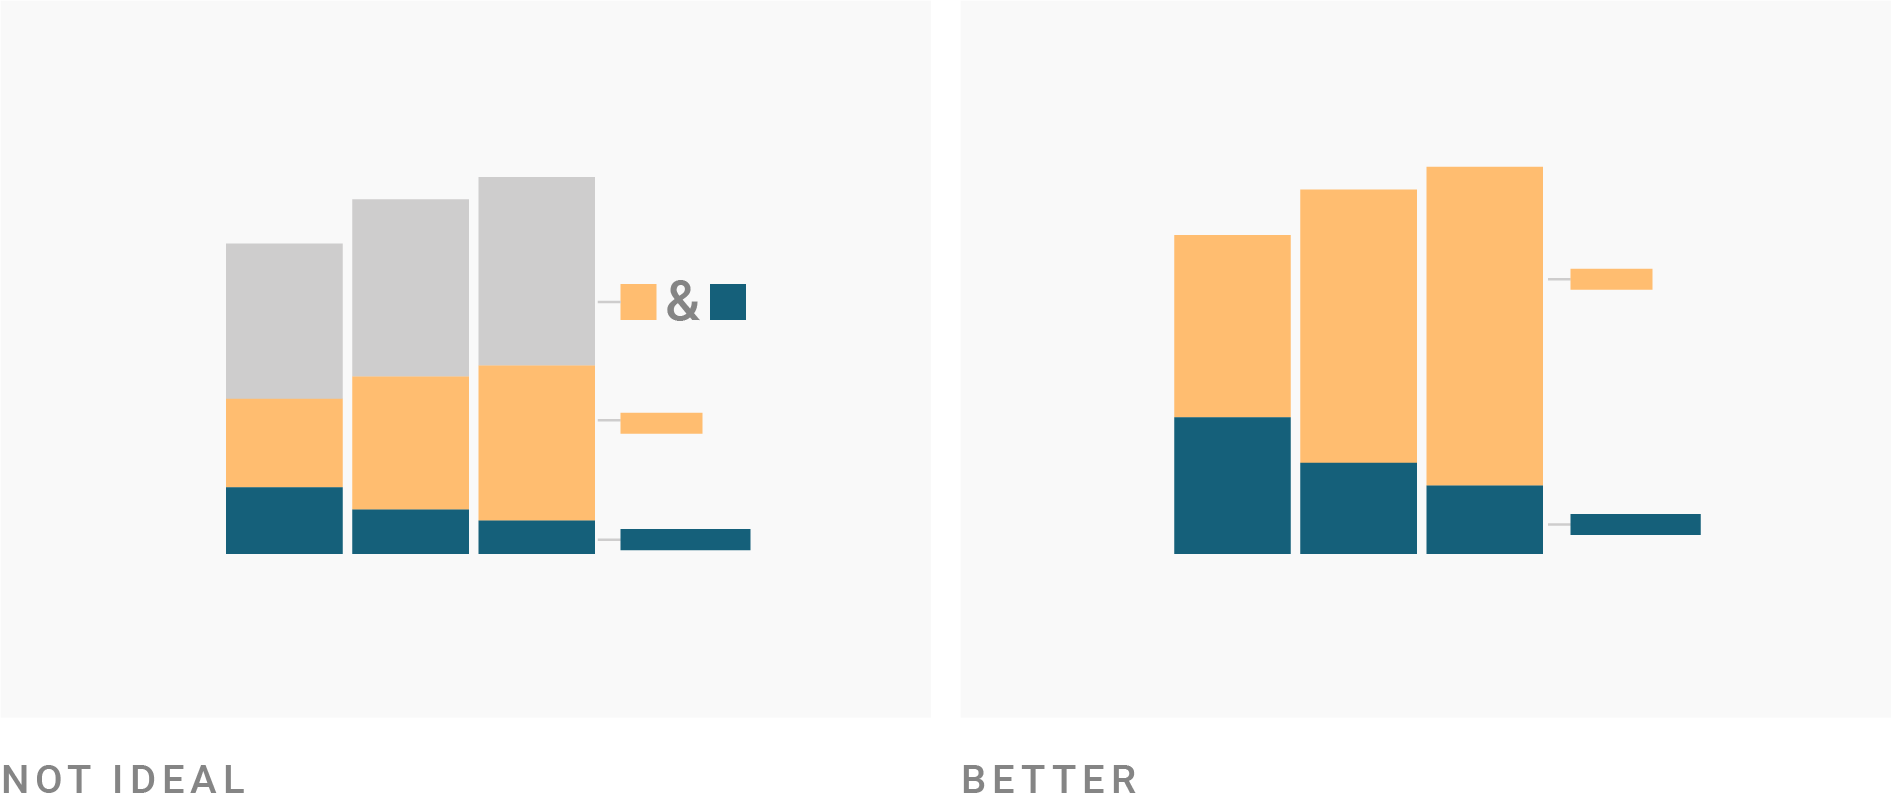
\includegraphics[width=\linewidth]{images/bar-chart/stacked-column-refinement-43-only-parts.png}
        \fullwidthfigurecaption{Include all parts of the whole, and only parts of the whole; do not add a total segment to a stacked chart that already encodes the total by full bar height.}
        \label{fig:stacked-bar-refinement-b}
        \label{fig:stacked-bar-refinement-b-only-parts}
    \end{minipage}
    \hfill
    \begin{minipage}[t]{0.48\linewidth}
        \centering
        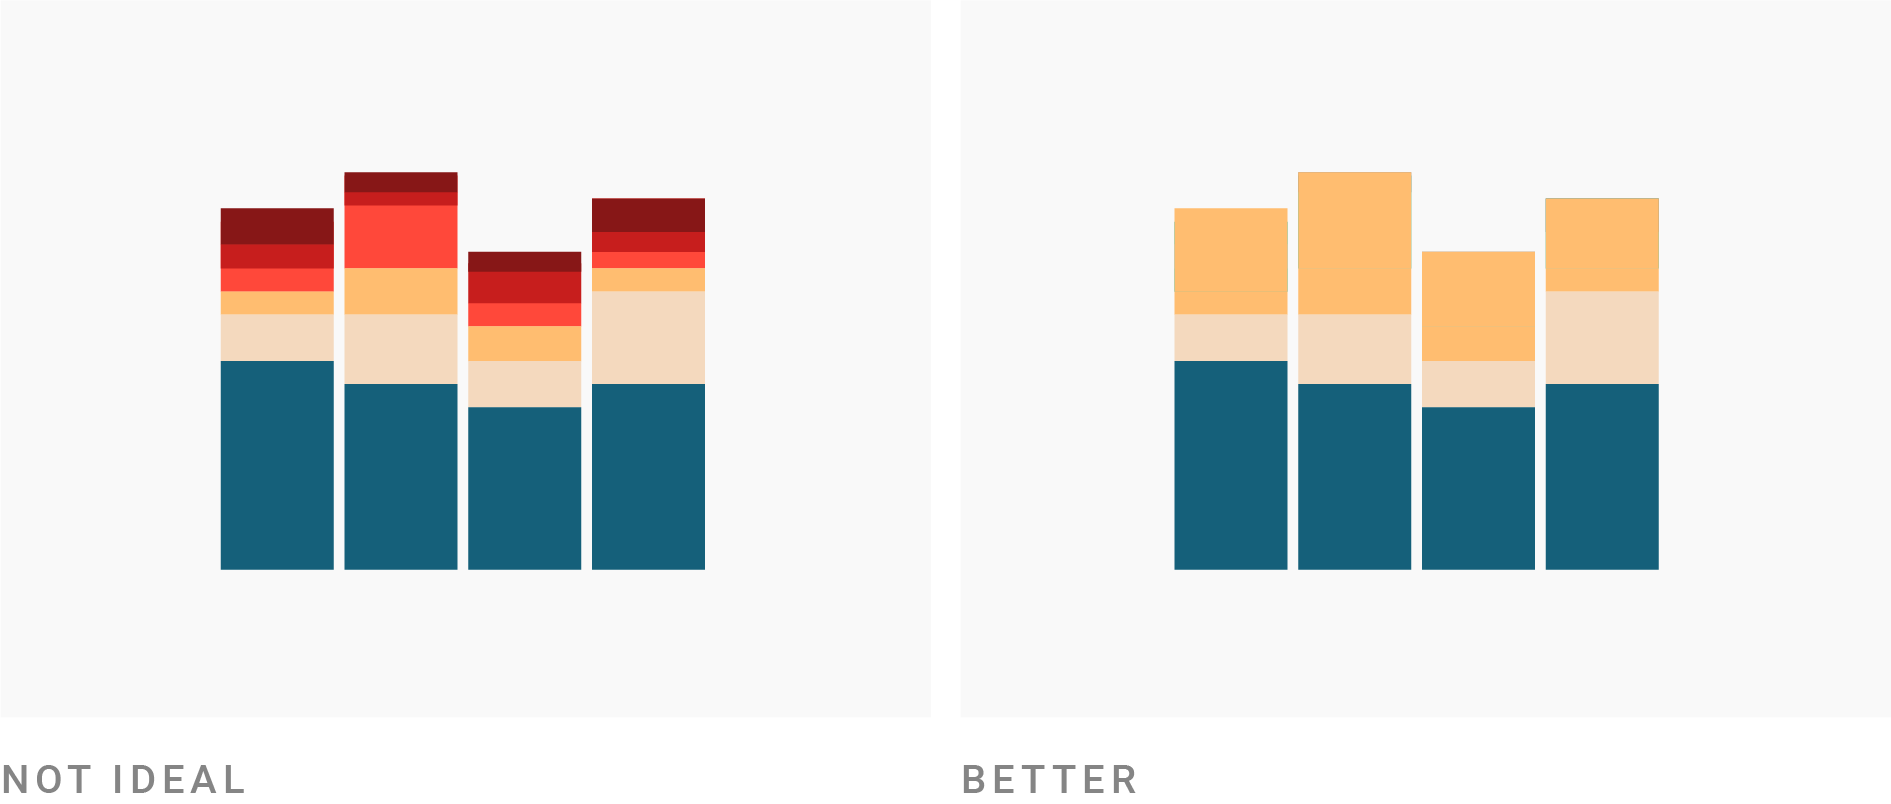
\includegraphics[width=\linewidth]{images/bar-chart/stacked-column-refinement-45-group-others.png}
        \fullwidthfigurecaption{Group tiny categories into ``Others'' so important segments remain salient and labels stay manageable.}
        \label{fig:stacked-bar-refinement-b-group-others}
    \end{minipage}
\end{figure*}

\subsection{Dot Plots}
\paragraph{Brief}
A dot plot (sometimes called a dumbbell chart, barbell chart, or gap chart) is a strong alternative to paired or stacked bar charts. 
%Following the tradition developed by William Cleveland, i
It uses symbols (often circles) 
%at data values 
and can connect paired points with a line or an arrow. Data values map to one axis and groups to the other axis.
\margincitebox[Dot Plot References]{datawrapper_dot_plot_examples}

\whatpill\  A simple dot plot maps one \textbf{quantitative value attribute} per \textbf{item}, with an optional \textbf{categorical key attribute} for grouping. A connected dot plot adds another quantitative value per item to express change between two states.

\whypill\  The main \textit{actions} are \textbf{query} (precise value comparison), \textbf{search} (outliers and ranges), and \textbf{analyse} (direction/size of change in connected variants).
%\parencite{heer2010}. 
The primary \textit{targets} are value differences, ranges, and anomalies.

\howpill\  At the \textbf{idiom} level, the \textit{mark} is a \textbf{point}; the dominant \textit{channel} is the \textbf{position on a common scale}, which is highly effective for ordered comparison. Connected variants add a line or arrow mark to encode change; \textbf{scalability} is typically from a few to hundreds of items.

\begin{figure*}[htbp]
    \centering
    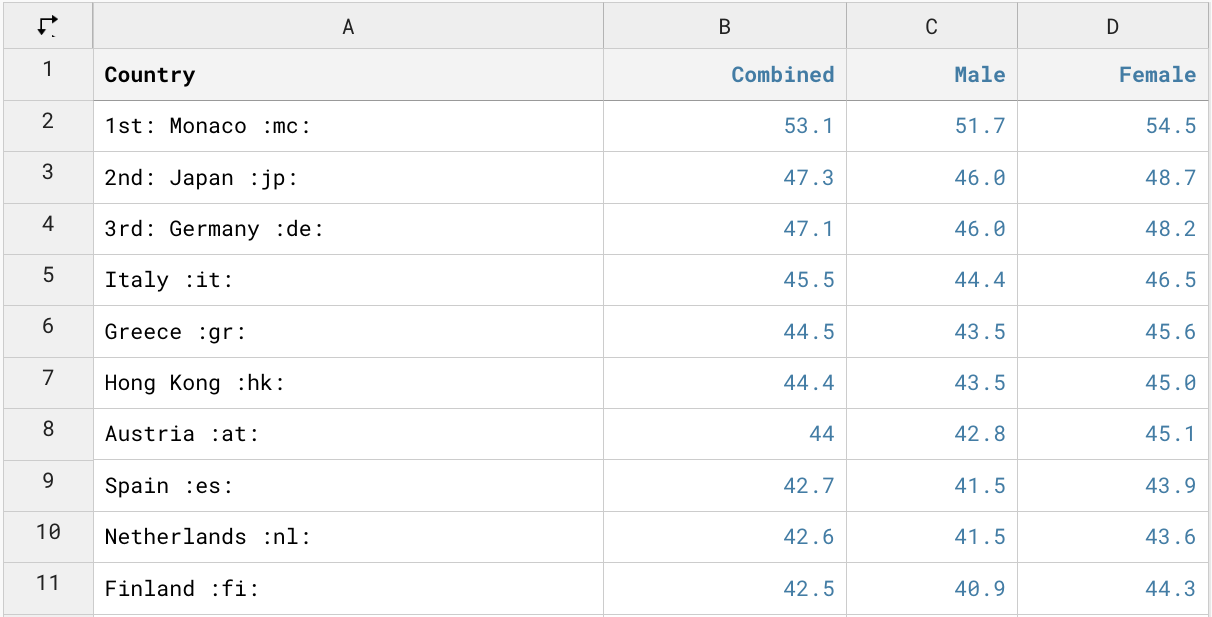
\includegraphics[width=0.52\linewidth]{images/dot-plot/dot-plot-datawrapper-example-1.png}\hfill
    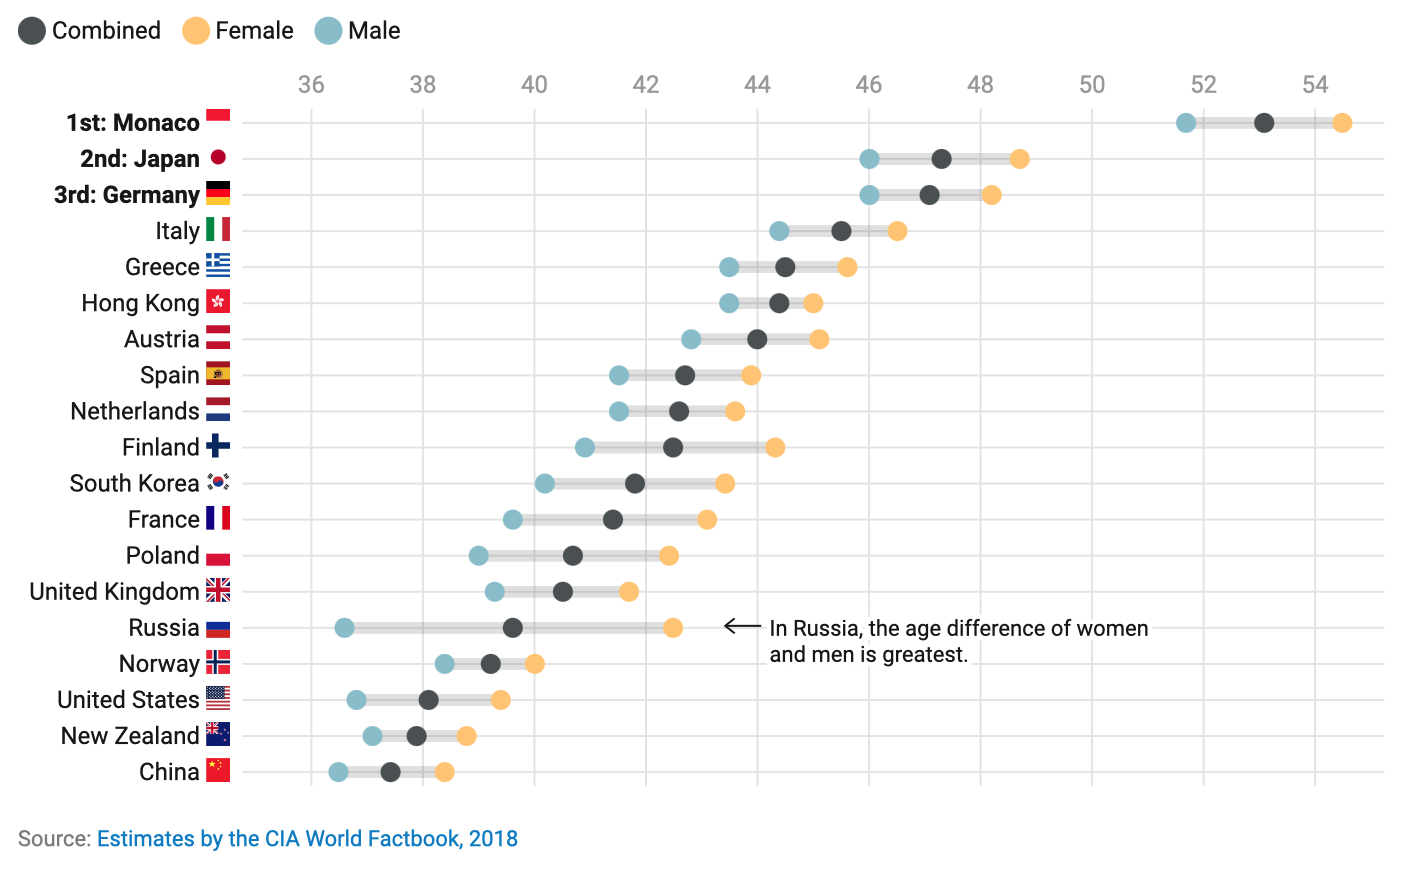
\includegraphics[width=0.46\linewidth]{images/dot-plot/dot-plot-datawrapper-example-2.png}
    \caption{Dot-plot guidance (Datawrapper): use dot plots for precise low-ink comparison, connected dots for before/after gap reading, and sorting for fast ranking scans.}
    \label{fig:dot-plot-examples}
\end{figure*}


\subsection*{Design Guide}
\paragraph{Use when}
\begin{itemize}
    \item \textit{Many-category comparison with less clutter.} Dot plots are effective when we need bar-like comparison but with lower visual weight and more whitespace.
    \item \textit{Two-value comparison per category.} Connected dot plots 
    %(dumbbell style) 
    are useful for showing before/after values, gap size, and direction.
    \item \textit{Sorted ranking with compact labels.} Sorting by value helps readers scan categories quickly, similar to sorted bar charts but with less ink.
\end{itemize}

\paragraph{Avoid when}
\begin{itemize}
    \item \textit{Highly volatile time series.} Dot plots summarise endpoints (or sparse checkpoints) and can hide strong intermediate fluctuations; line charts are better when full temporal trajectory matters.
    %\item \textit{Over-annotation and category overload.} If too many labels, colors, or symbols are added, the low-ink advantage disappears and the chart becomes difficult to parse.
    \item \textit{Direction is unclear without visual guidance.} In paired comparisons, readers may miss which side is higher unless direction is made explicit. Use clear colour contrast, sorting, group splitting, or arrows when direction-of-change is central.
    \item \textit{No shared scale/baseline for comparison.} As with bars, meaningful comparison still depends on a consistent axis scale.
\end{itemize}

%\paragraph{Wrap up}
%In summary, dot plots are a versatile alternative to bars for dense category comparison and paired gap-reading. The key refinement suggestions are: see Figure~\ref{fig:dot-plot-examples} and its caption.


\section{Idiom: Line Charts}
\margincitebox[Line Chart References]{munzner2014,kirk2019}
\paragraph{Brief}
A line chart is 
%a statistical idiom
built from points connected by lines in a Cartesian coordinate system. It is primarily used to show how values change over time or across ordered categories.

\whatpill\  A line chart uses one \textbf{ordered key attribute} (often time) and one \textbf{quantitative value attribute} per \textbf{item}. Optional series grouping adds one \textbf{categorical key attribute}.

\begin{figure*}[htbp]
    \centering
    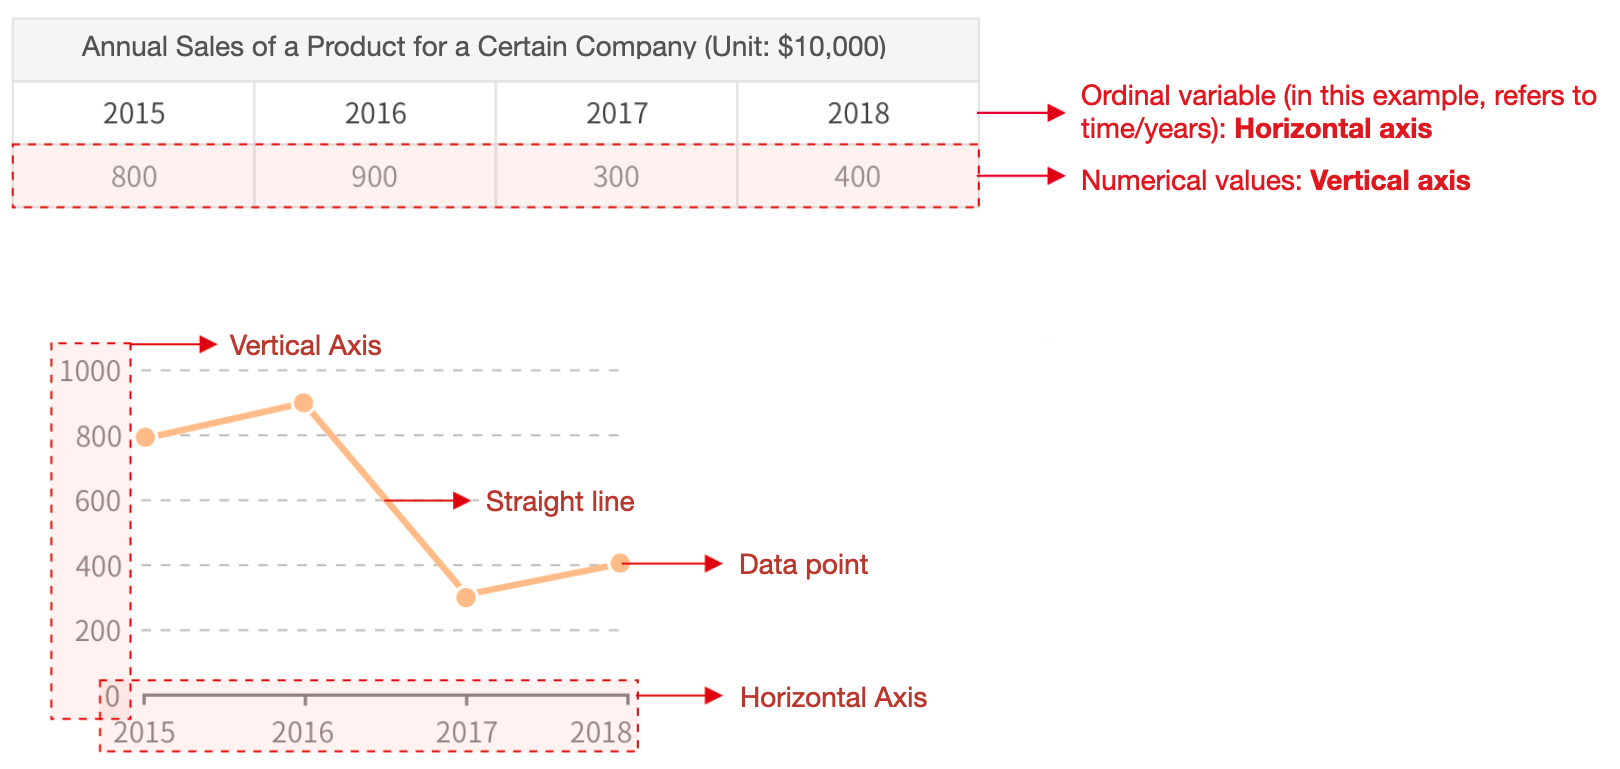
\includegraphics[width=0.92\linewidth]{images/line-chart/line-chart-elemental-composition.png}
    \caption{Elemental composition of a line chart: ordered x-axis, quantitative y-axis, points and connecting line.}
    \label{fig:line-chart-elemental-composition}
\end{figure*}

\whypill\  The main \textit{task} is \textbf{analyse}, and the primary \textit{target} is \textbf{trend} over an ordered sequence. Secondary \textit{actions} are \textbf{search} (peaks/troughs, turning points) and \textbf{query} (specific values).

\howpill\  At the \textbf{idiom} level, the main \textit{mark} is \textbf{line} (optional \textbf{point} marks for samples). The key \textit{channels} are \textbf{horizontal position} for ordered keys and \textbf{vertical position} for quantitative values. In \textbf{form} terms, interaction (zoom/highlight) improves readability when series count grows.

\subsection*{Design Guide}
\margincitebox[Design Guidance Sources]{datawrapper_line_chart_guidance}
\paragraph{Use when}
\begin{itemize}
    \item \textit{One variable over time or ordered stages.} Line charts are effective for showing a single series evolving across ordered positions .
    \item \textit{Multiple ordered series comparison.} Line charts can compare multiple variables across the same ordered axis and highlight convergence/divergence or crossover.
\end{itemize}

% \begin{figure*}[htbp]
%     \centering
%     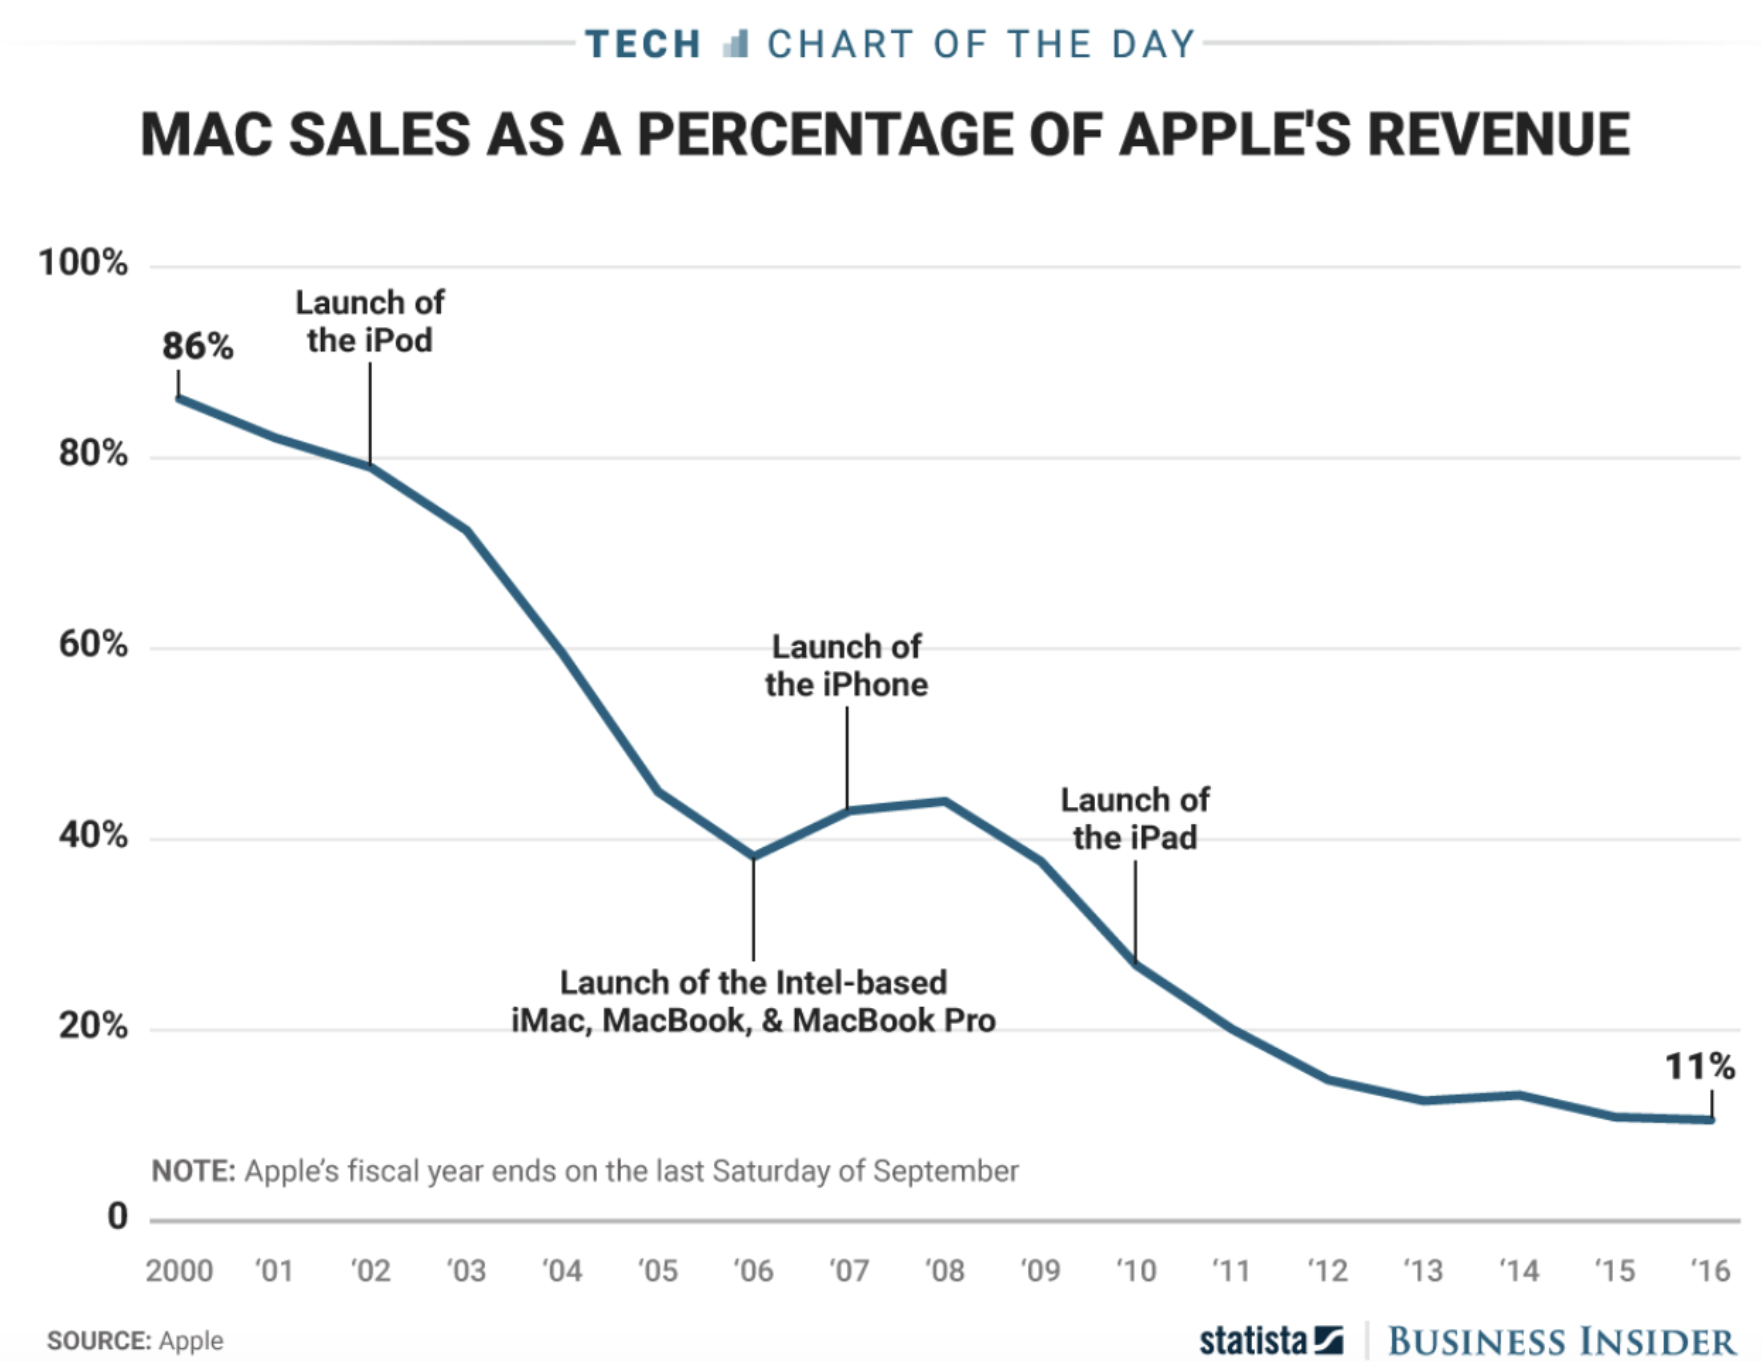
\includegraphics[width=0.48\linewidth]{images/line-chart/line-chart-applicable-time-trend.png}\hfill
%     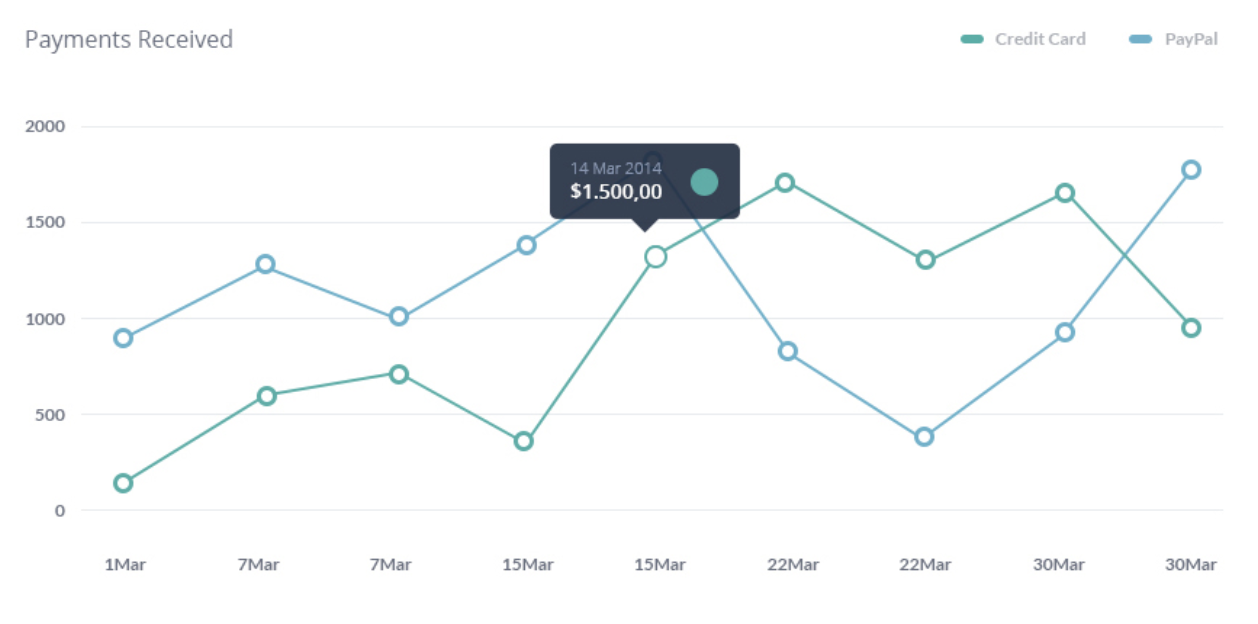
\includegraphics[width=0.48\linewidth]{images/line-chart/line-chart-applicable-multi-series.png}
%     \caption{Applicable scenarios for line charts: one ordered series showing trend over time (left), and multiple series compared across the same ordered axis (right).}
%     \label{fig:line-chart-applicable-scenarios}
% \end{figure*}

\paragraph{Avoid when}

% \begin{marginfigure}
%     \centering
%     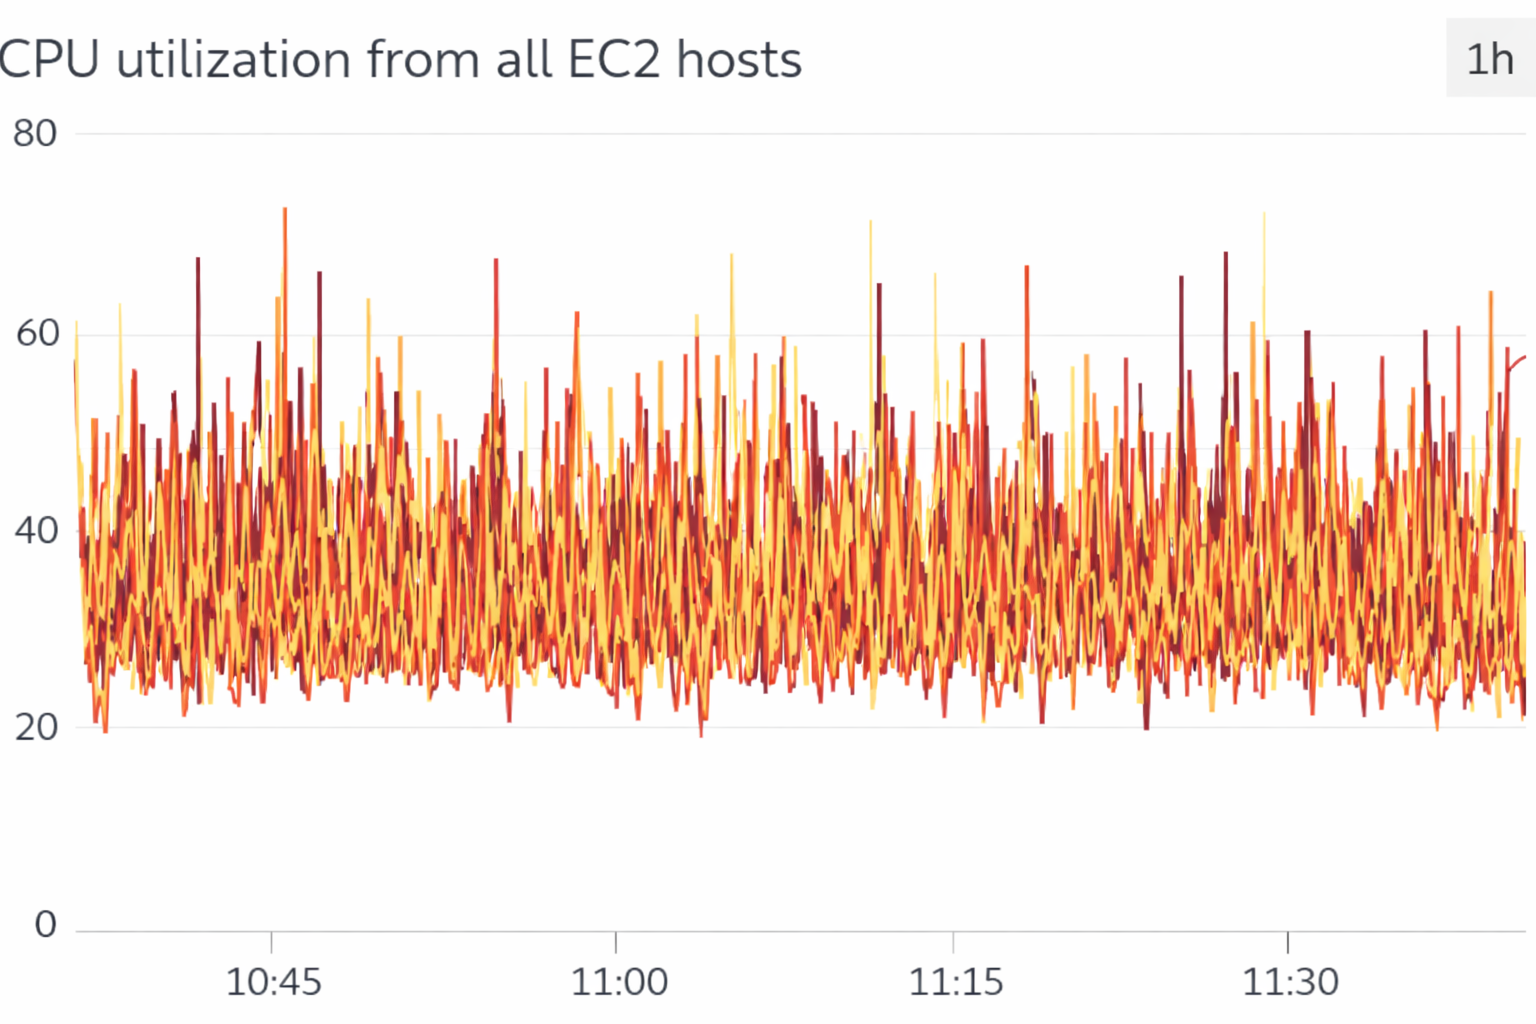
\includegraphics[width=\linewidth]{images/line-chart/line-chart-inapplicable-too-many-x-nodes.png}
%     \caption{Inapplicable scenario: too many x-axis nodes reduce readability.}
%     \label{fig:line-chart-inapplicable-too-many-x}
% \end{marginfigure}

\begin{marginfigure}
    \centering
    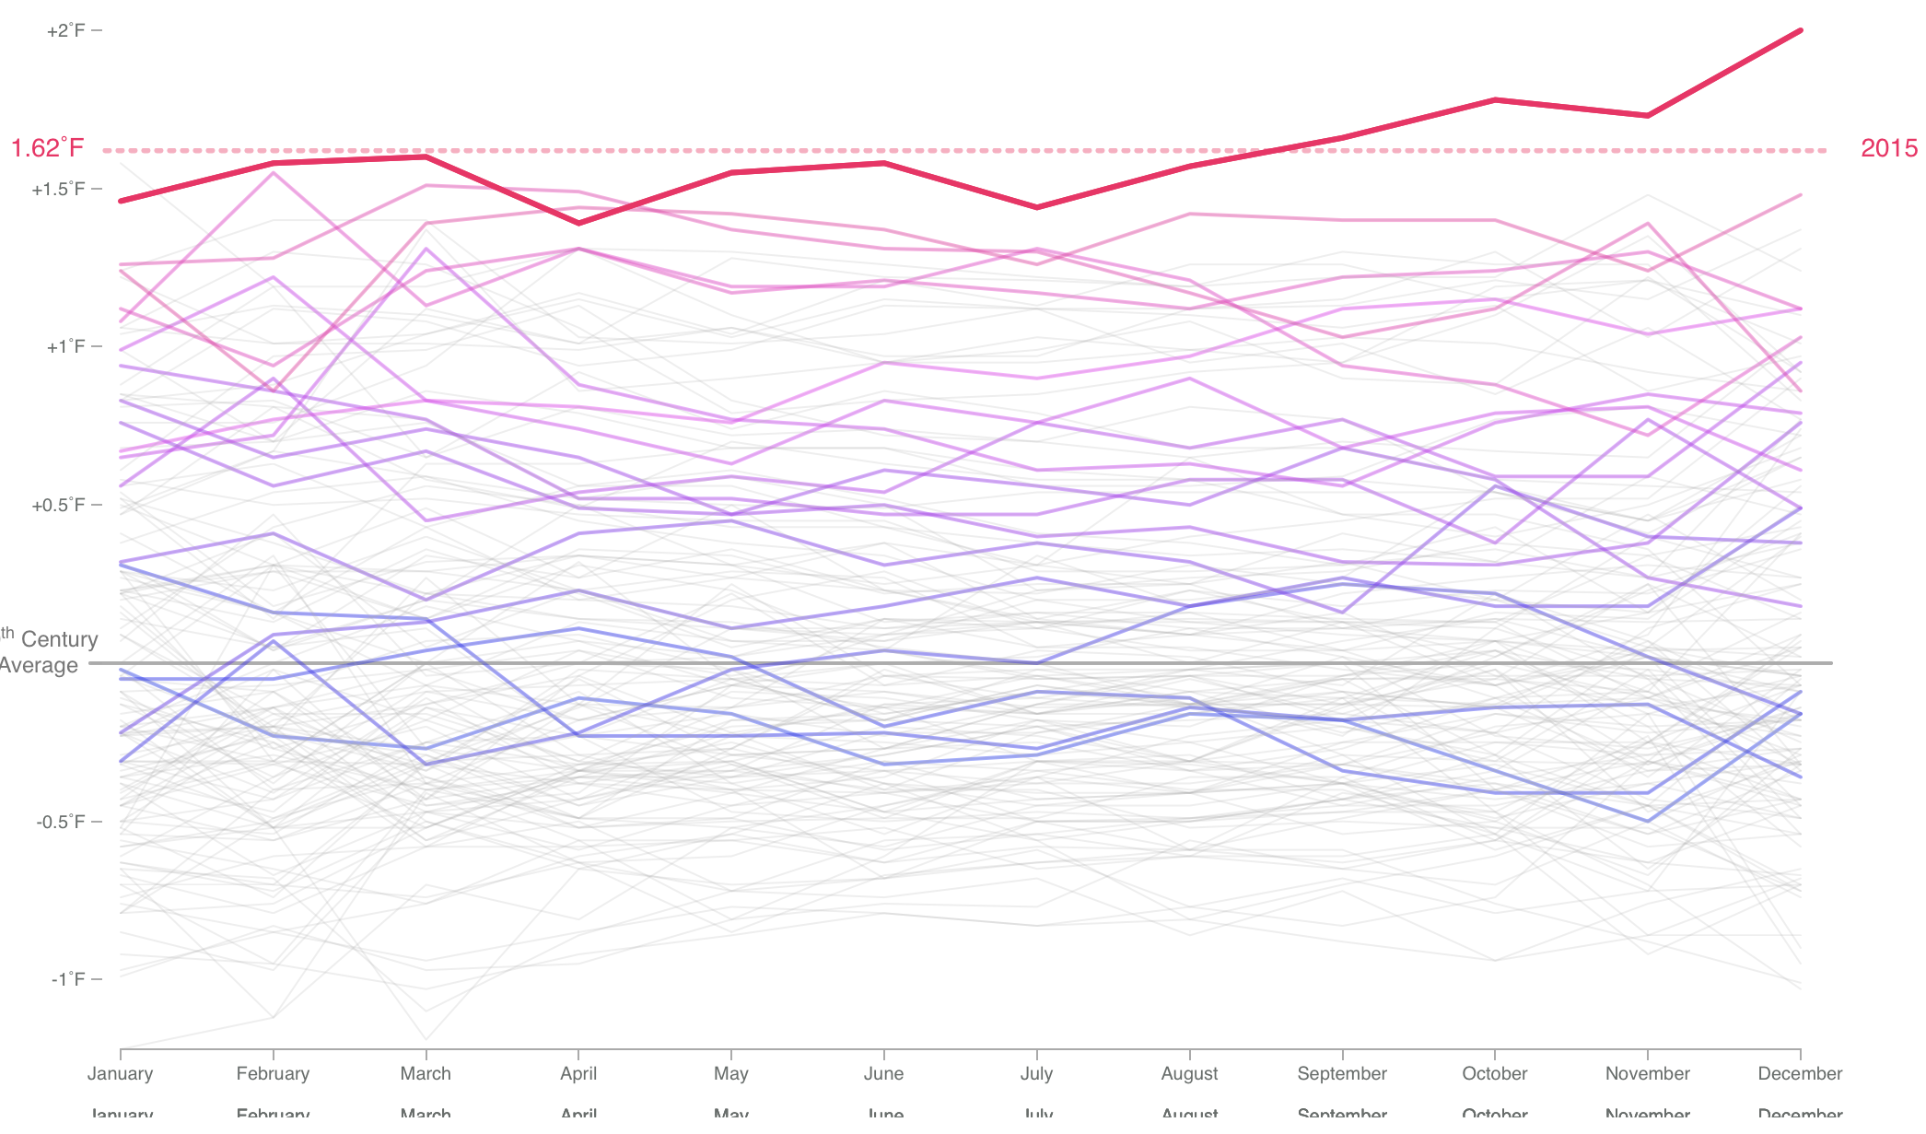
\includegraphics[width=\linewidth]{images/line-chart/line-chart-inapplicable-too-many-lines.png}
    \caption{Inapplicable scenario: too many line series create clutter and overplotting. A representative case is Bloomberg's 1880--2017 global temperature graphic, which maps each year to one monthly-temperature line and produces a dense line field. A practical remedy is progressive reveal, filtering, and muted context styling so only key years stand out \parencite{bloomberg_hottest_year_2018}.}
    \label{fig:line-chart-inapplicable-too-many-lines}
\end{marginfigure}

\begin{itemize}
    \item \textit{Too many samples.} If there are too many ordered positions, labels and local variation become unreadable.
    \item \textit{Too many lines.} When the dataset contains too many series, overplotting makes it hard to focus on the key message (see Figure~\ref{fig:line-chart-inapplicable-too-many-lines}).
    \item \textit{Unordered categories.} If x-axis categories are nominal (unordered), connecting points implies continuity that does not exist; bar charts are usually better.
    \item \textit{Misleading axis framing.} Line charts should show the zero y-baseline, but sometimes 
    %. Use zero when distance-to-zero is the message; otherwise,
    a focused y-range can better reveal trend, slope, and local variation (see Figures~\ref{fig:line-chart-scale-comparisons} and~\ref{fig:line-chart-axis-zero-vs-focused}).
    %\item \textit{Crash-to-bottom metaphors.} When the bottom boundary is visually strong, a declining line can appear to ``hit the floor'' even far above zero. Reduce this by slightly extending the y-range and de-emphasizing bottom-axis cues (see Figure~\ref{fig:line-chart-axis-metaphor-fixes-b}).
    %\margincitebox[]{infragistics_line_axis_examples}
    \item \textit{Unclear horizontal cropping.} Truncating the x-axis removes data, not just whitespace. State the time window and why it was chosen so readers can judge representativeness.
\end{itemize}

\begin{figure*}[htbp]
    \centering
    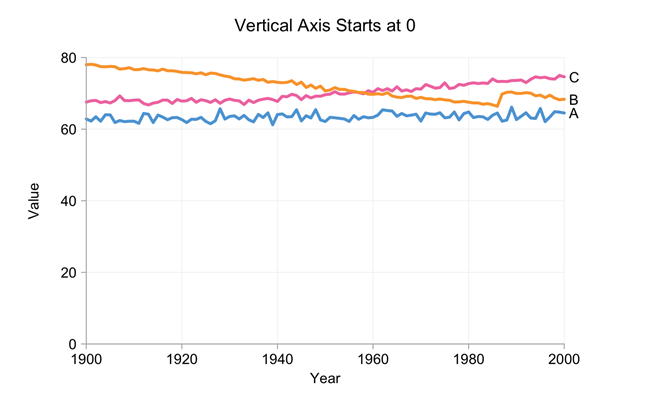
\includegraphics[width=0.48\linewidth]{images/line-chart/line-chart-axis-zero-start.png}\hfill
    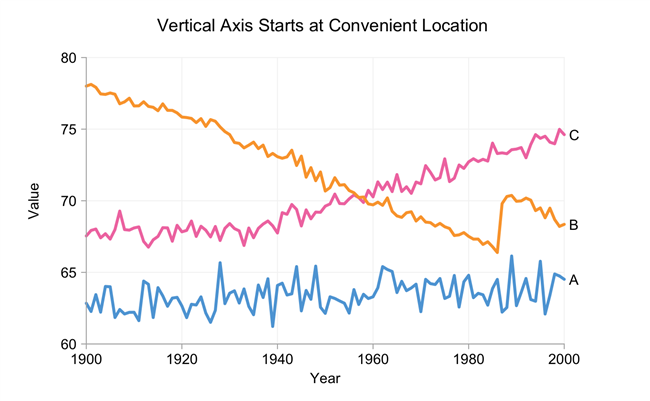
\includegraphics[width=0.48\linewidth]{images/line-chart/line-chart-axis-focused-range.png}
    \caption{Line-chart axis framing: zero-start emphasizes distance to zero (left), while focused range increases resolution for trend and local variation when values are far from zero (right).}
    \label{fig:line-chart-axis-zero-vs-focused}
\end{figure*}

%\begin{figure*}[htbp]
%    \centering
%     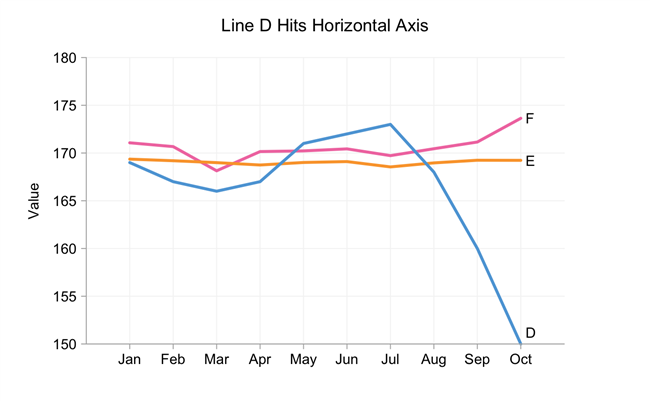
\includegraphics[width=0.49\linewidth]{images/line-chart/line-chart-axis-bottom-crash-problem.png}\hfill
%    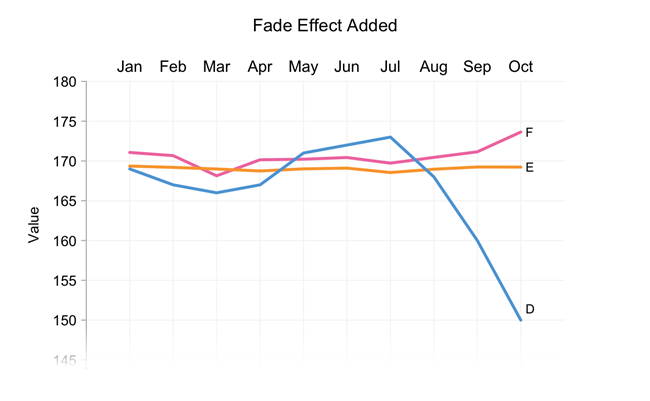
\includegraphics[width=0.49\linewidth]{images/line-chart/line-chart-axis-fade-effect.png}
%    \caption{Stepwise crash-metaphor fix: start from the misleading ``line hits the floor'' view (left), then slightly extend the y-range, reduce bottom-axis salience, move month labels to the top, and optionally add a subtle bottom fade for the final view (right) \parencite{infragistics_line_axis_examples}.}
%    \label{fig:line-chart-axis-metaphor-fixes-b}
%\end{figure*}

%\paragraph{Wrap up}
%In summary, line charts are effective for ordered change, but clarity depends on disciplined styling and annotation choices. The key refinement suggestions are:

\paragraph{Refinements}
\begin{figure*}[htbp]
    \centering
    \begin{minipage}[t]{0.48\linewidth}
        \centering
        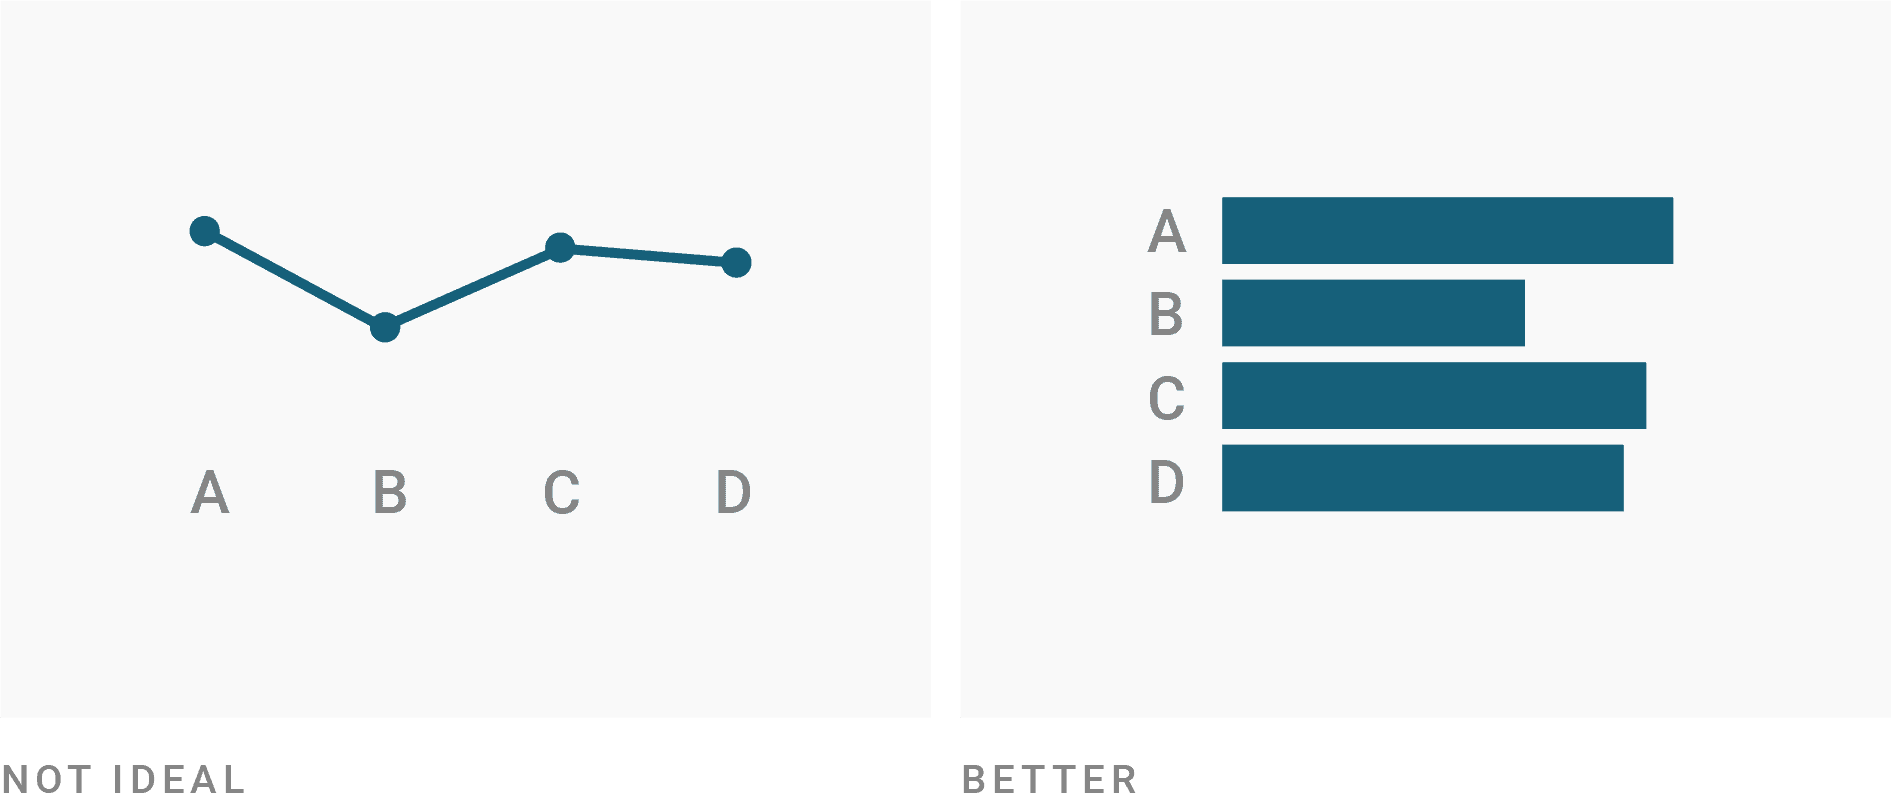
\includegraphics[width=\linewidth]{images/line-chart/line-chart-bar-vs-line-choice.png}
        \fullwidthfigurecaption{Choosing bar vs line: if the key attribute is categorical, bar charts are usually more appropriate; if the key attribute is ordered, especially time, line charts are generally preferred.}
        \label{fig:line-chart-choice-comparisons}
        \label{fig:line-chart-choice-bar-vs-line}
    \end{minipage}
    \hfill
    \begin{minipage}[t]{0.48\linewidth}
        \centering
        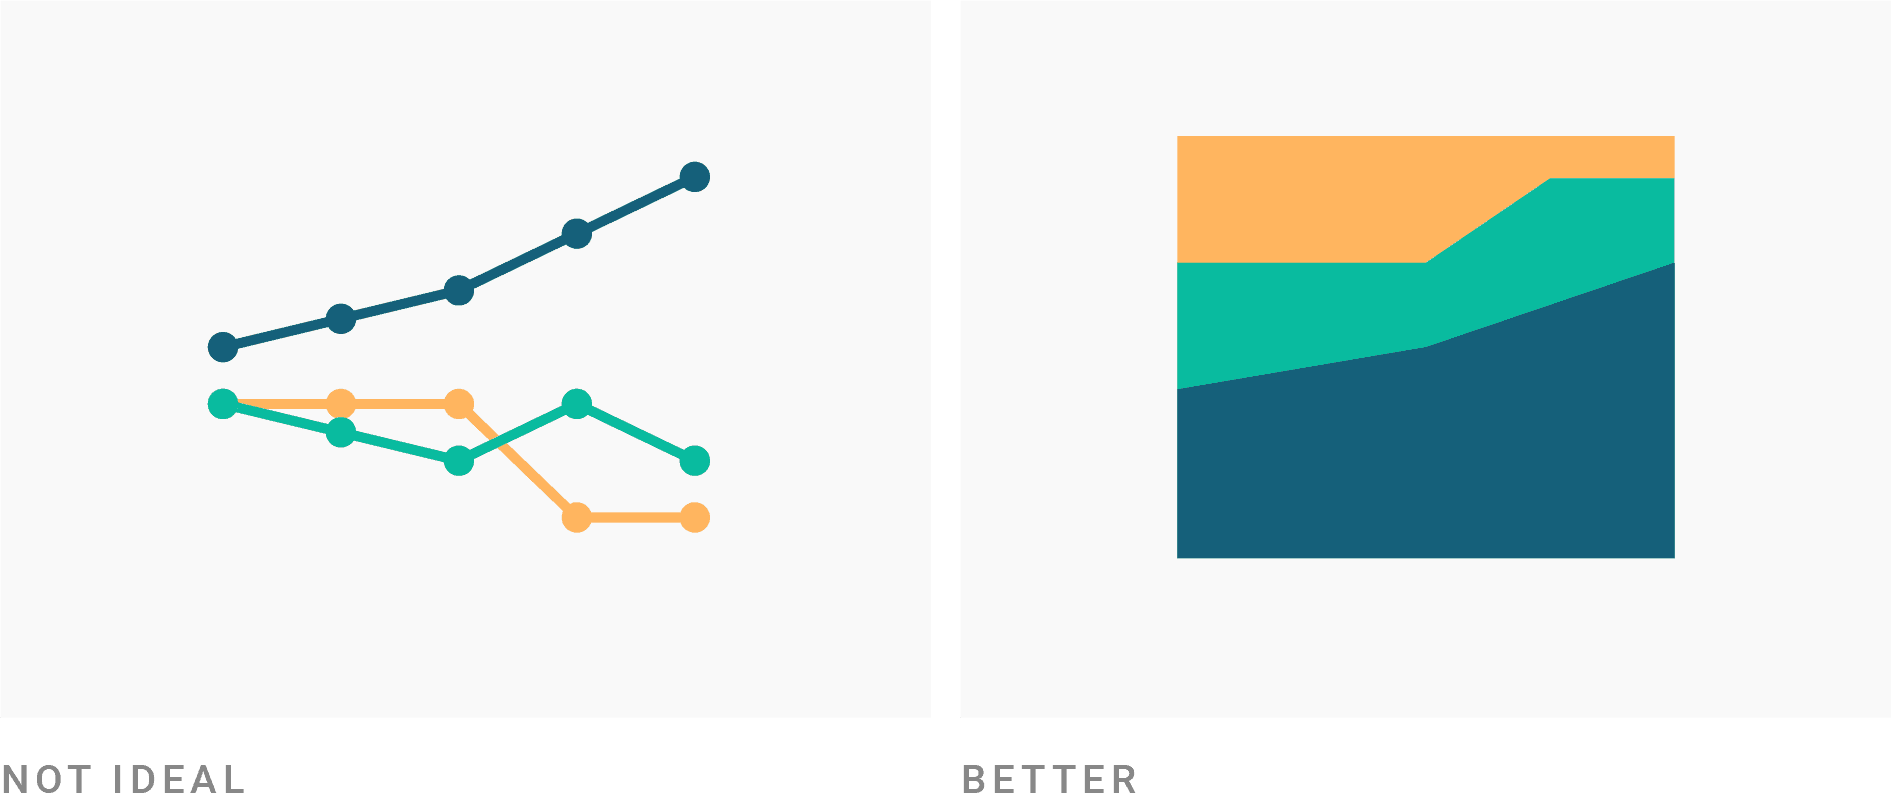
\includegraphics[width=\linewidth]{images/line-chart/line-chart-line-vs-area-sum-important.png}
        \fullwidthfigurecaption{Line vs area for composition: if readers need to see both category trajectories and their sum (especially shares approaching 100\%), area charts can be more direct than line charts.}
        \label{fig:line-chart-choice-line-vs-area}
    \end{minipage}
\end{figure*}

\begin{figure*}[htbp]
    \centering
    \begin{minipage}[t]{0.48\linewidth}
        \centering
        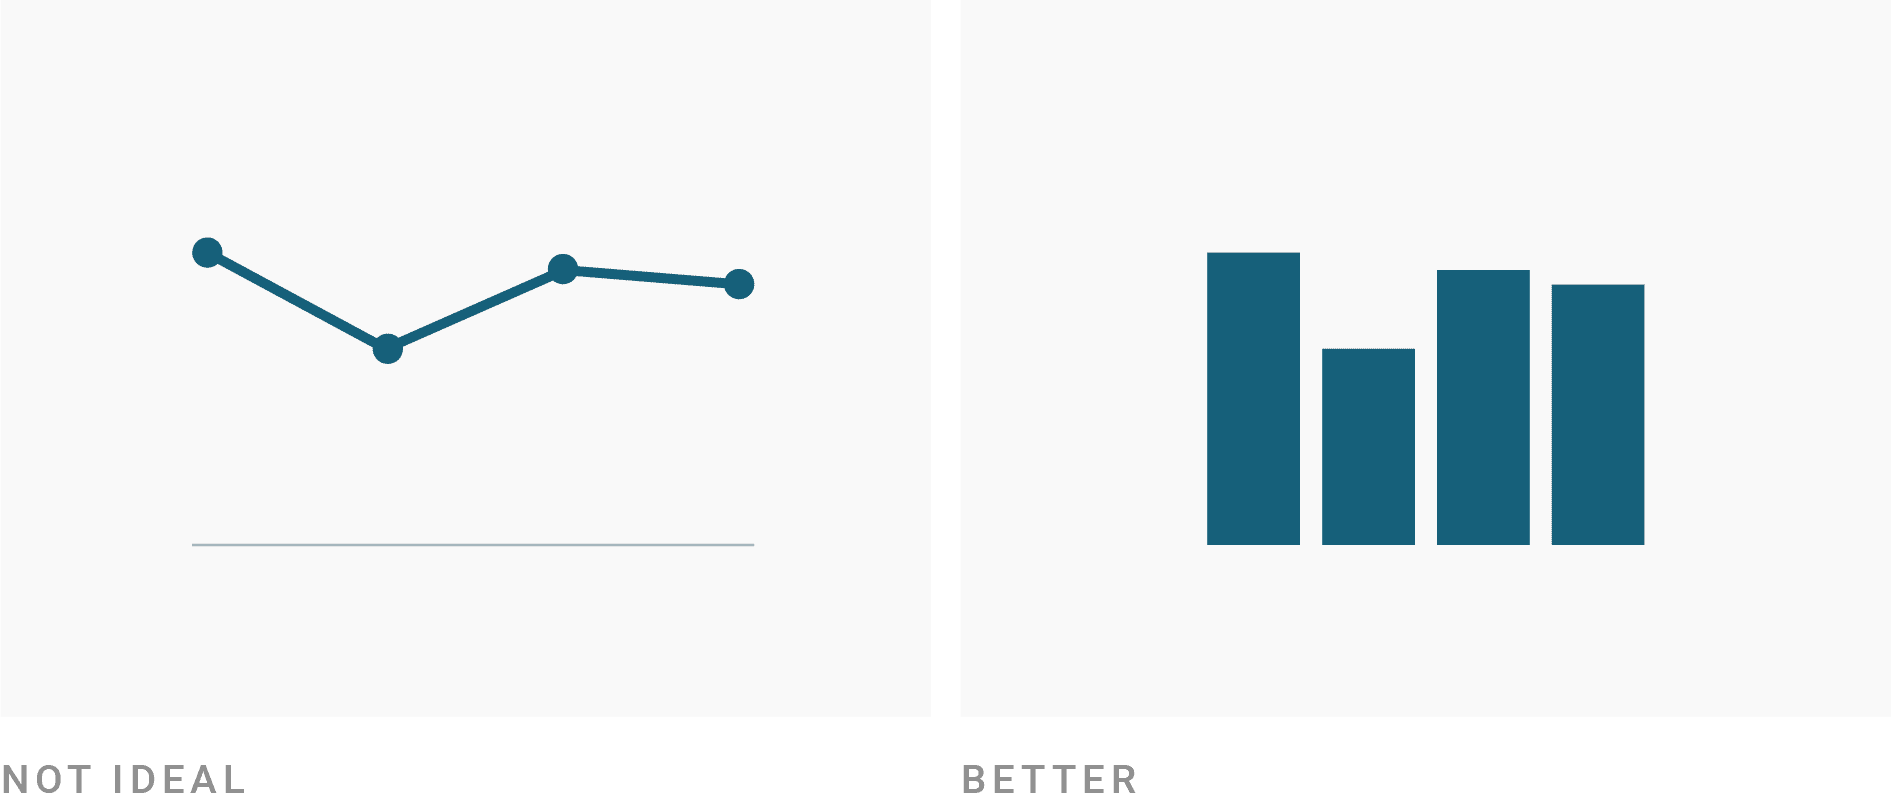
\includegraphics[width=\linewidth]{images/line-chart/line-chart-few-points-vs-many-values.png}
        \fullwidthfigurecaption{Few points vs many values: for a few equally spaced values in one series, columns can be easier to compare; line charts are often stronger when values are numerous, irregularly spaced, or interpreted as continuous change.}
        \label{fig:line-chart-scale-comparisons}
        \label{fig:line-chart-scale-few-vs-many}
    \end{minipage}
    \hfill
    %\begin{minipage}[t]{0.48\linewidth}
   %     \centering
%        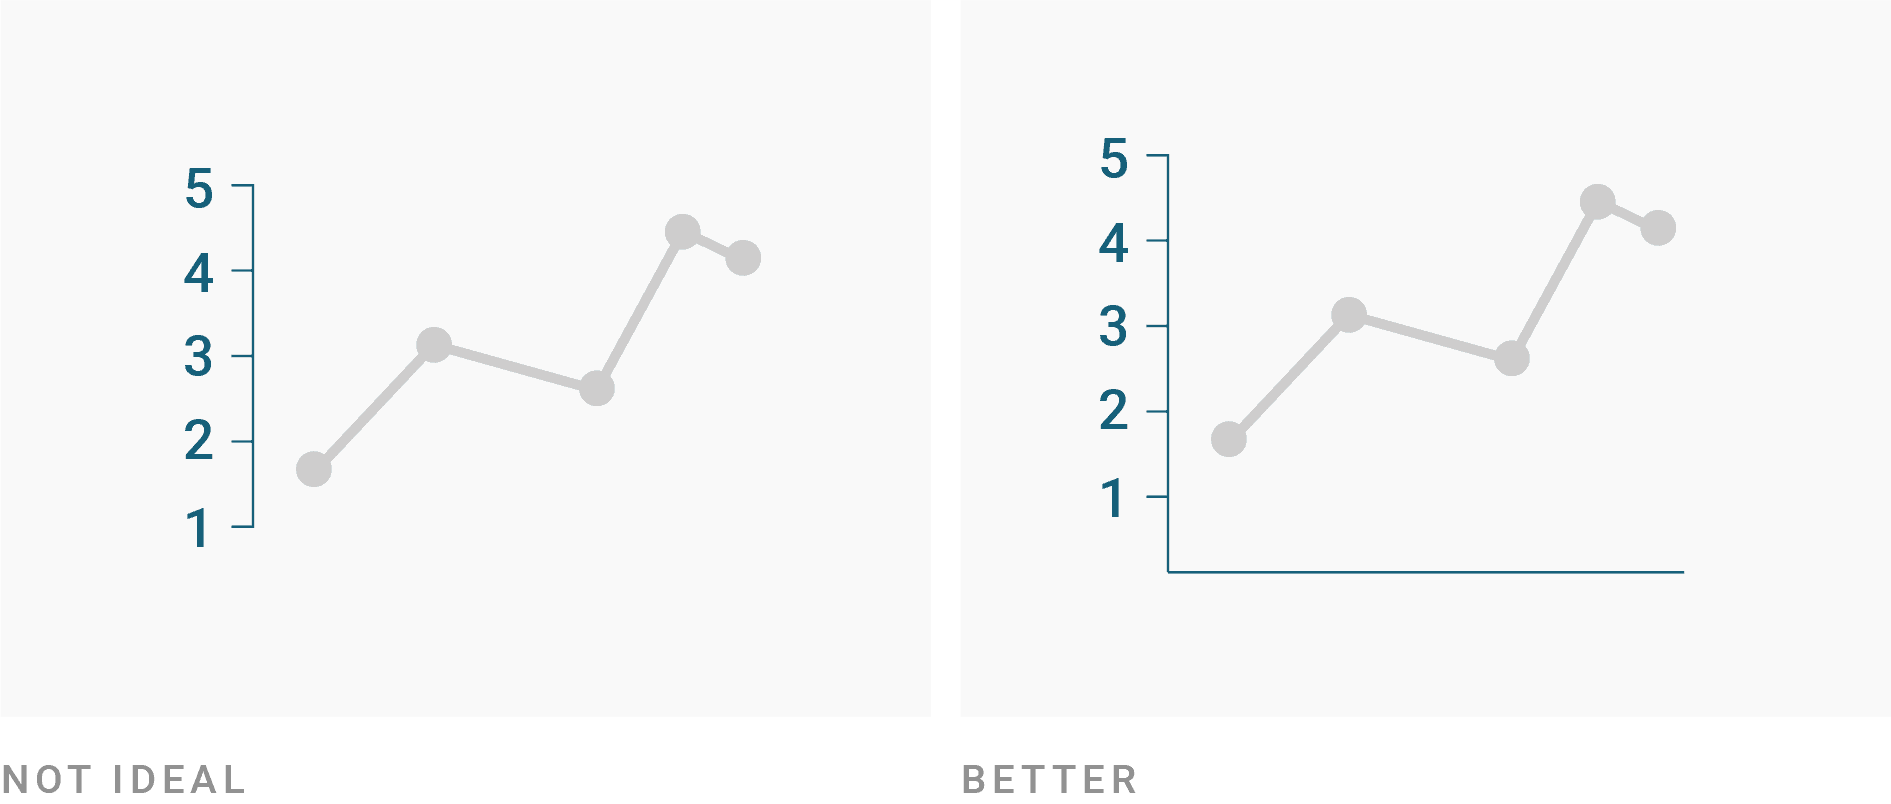
\includegraphics[width=\linewidth]{images/line-chart/line-chart-zero-baseline-when-near-zero.png}
%        \fullwidthfigurecaption{Line charts handle many or irregular intervals well; add a zero baseline only when near-zero reference is part of the interpretation task.}
%        \label{fig:line-chart-scale-zero-baseline}
%    \end{minipage}
\end{figure*}

\begin{figure*}[htbp]
    \centering
    \begin{minipage}[t]{0.48\linewidth}
        \centering
        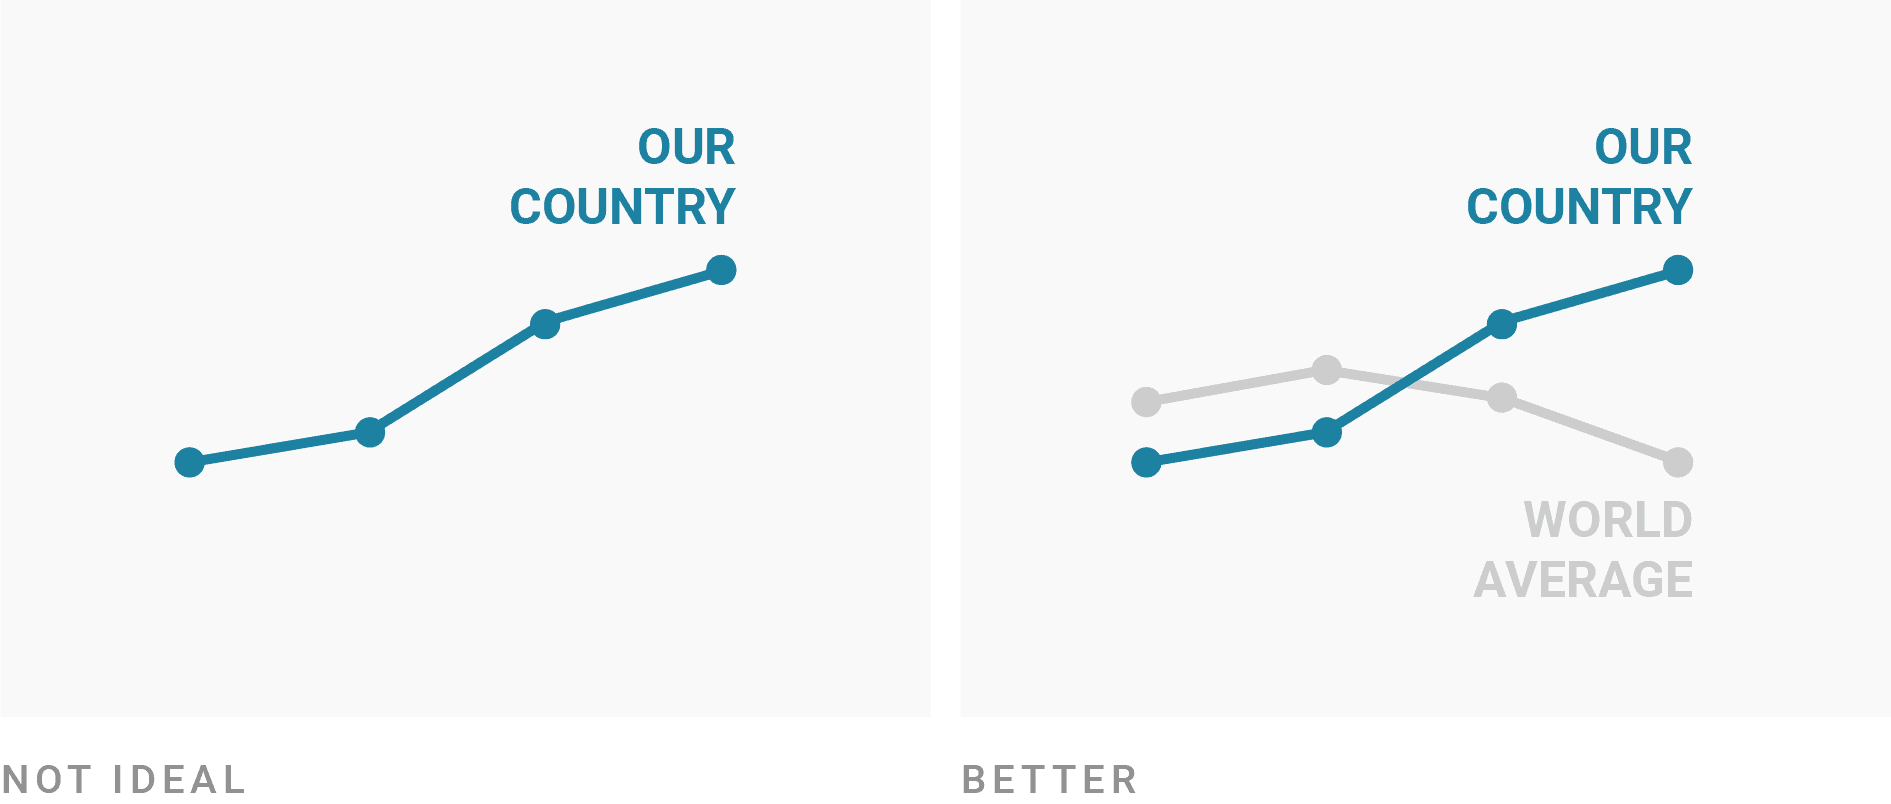
\includegraphics[width=\linewidth]{images/line-chart/line-chart-add-comparison-context.png}
        \fullwidthfigurecaption{Add comparison context such as averages, benchmarks, or peer series to help readers judge whether a pattern is high, low, typical, or exceptional.}
        \label{fig:line-chart-design-guidance-a}
        \label{fig:line-chart-design-guidance-a-comparison-context}
    \end{minipage}
    \hfill
    \begin{minipage}[t]{0.48\linewidth}
        \centering
        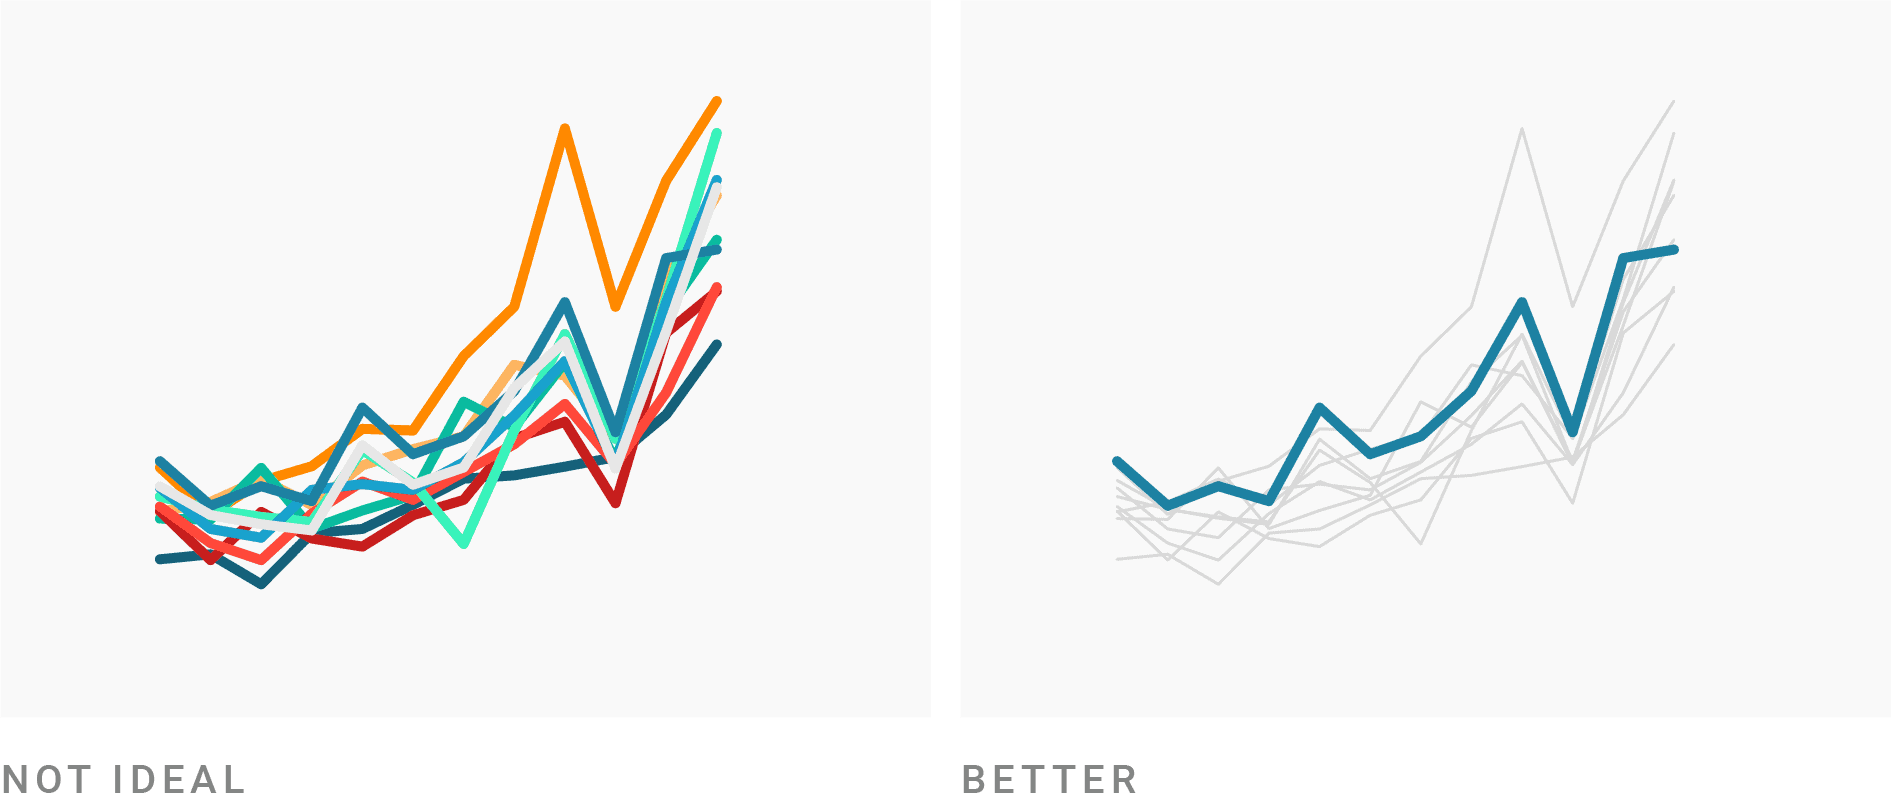
\includegraphics[width=\linewidth]{images/line-chart/line-chart-emphasis-by-style.png}
        \fullwidthfigurecaption{Use color, line width, and dash style to foreground the key series while muting context lines so attention stays on the main message.}
        \label{fig:line-chart-design-guidance-a-emphasis-style}
    \end{minipage}
\end{figure*}

\begin{figure*}[htbp]
    \centering
    \begin{minipage}[t]{0.48\linewidth}
        \centering
        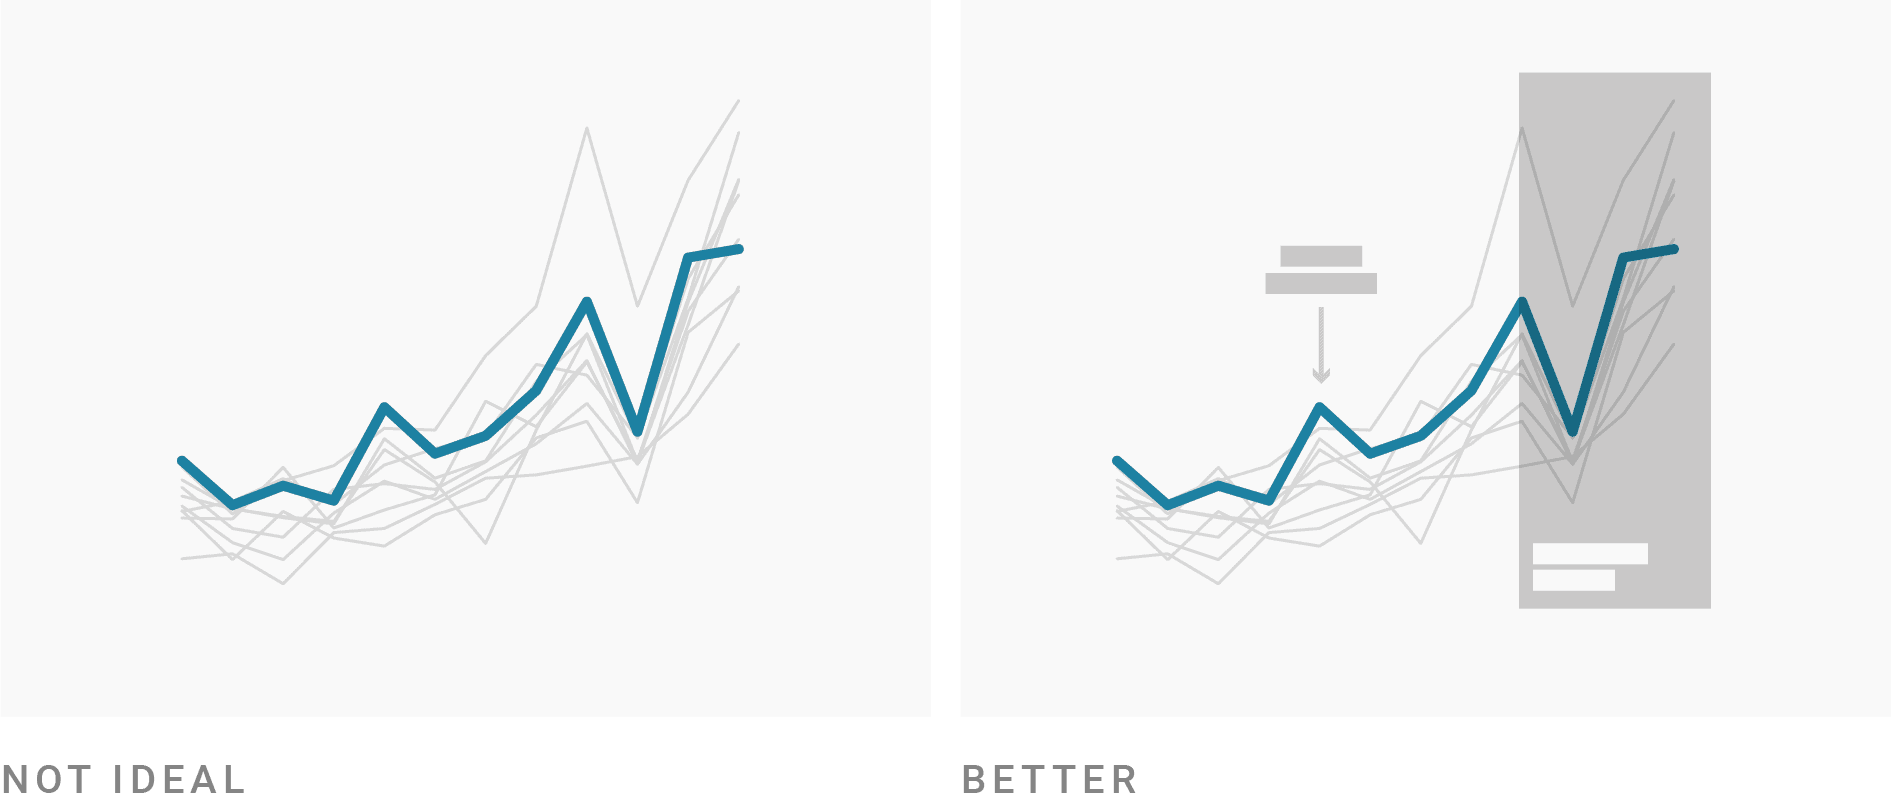
\includegraphics[width=\linewidth]{images/line-chart/line-chart-annotations-highlight-ranges.png}
        \fullwidthfigurecaption{Use concise annotations and highlighted ranges to explain events, interventions, or projection periods that drive visible changes.}
        \label{fig:line-chart-design-guidance-b}
        \label{fig:line-chart-design-guidance-b-annotations}
    \end{minipage}
    \hfill
    \begin{minipage}[t]{0.48\linewidth}
        \centering
        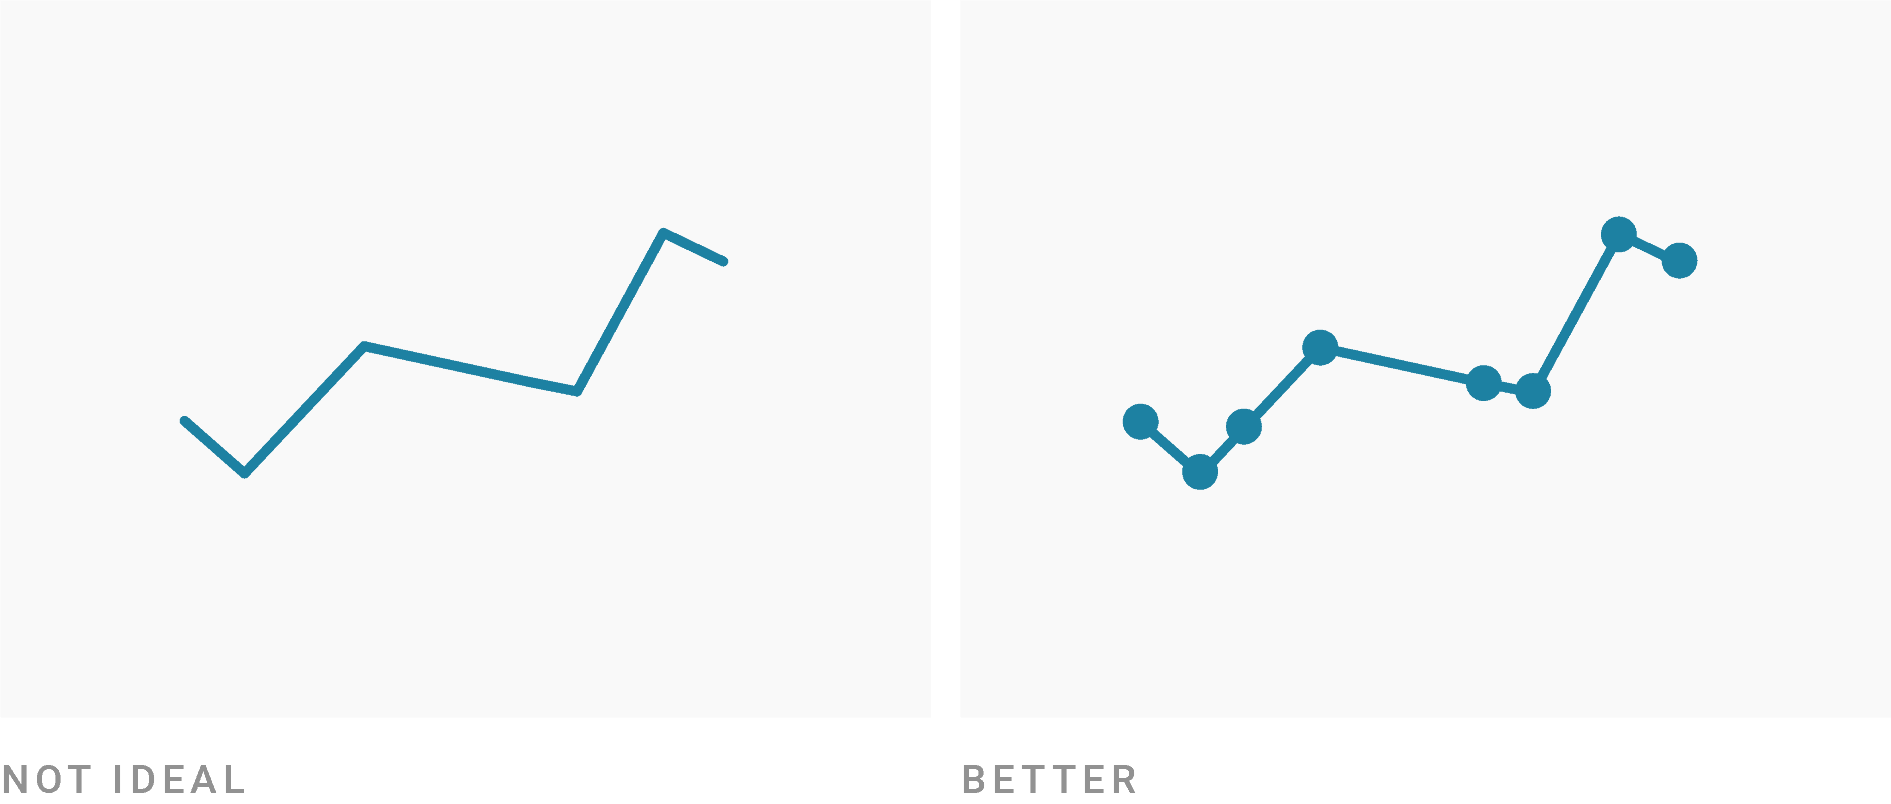
\includegraphics[width=\linewidth]{images/line-chart/line-chart-symbols-for-irregular-intervals.png}
        \fullwidthfigurecaption{Add point markers when dates are irregular or sampled so readers can see actual observation timing, but avoid dense symbols when intervals are regular.}
        \label{fig:line-chart-design-guidance-b-irregular-symbols}
    \end{minipage}
\end{figure*}

\begin{figure*}[htbp]
    \centering
    \begin{minipage}[t]{0.48\linewidth}
        \centering
        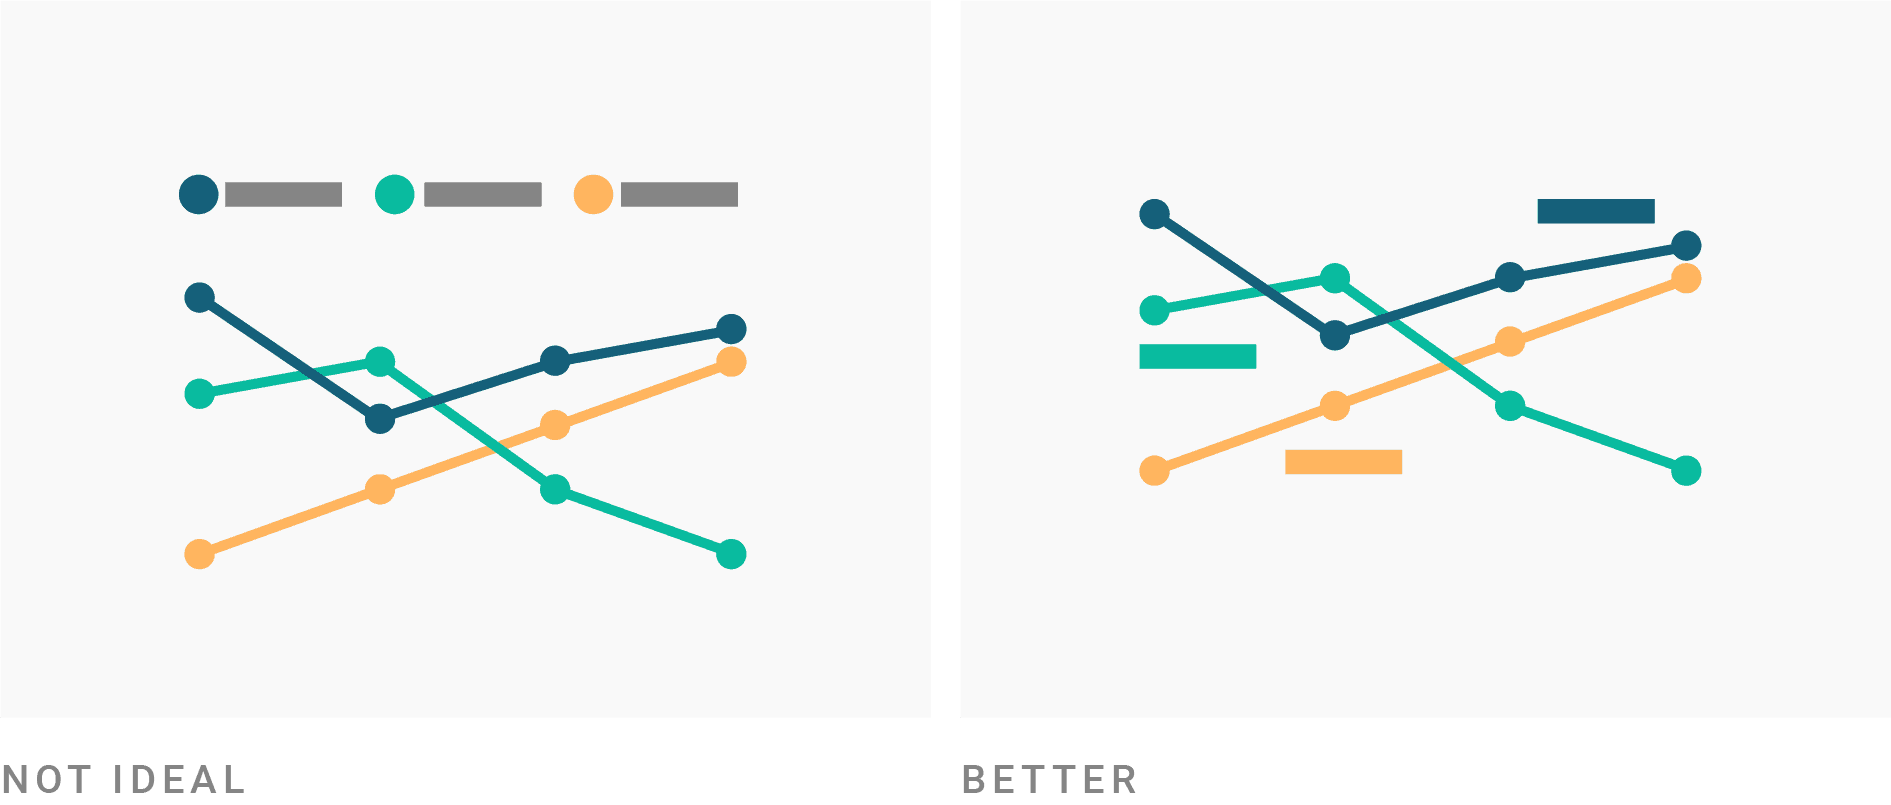
\includegraphics[width=\linewidth]{images/line-chart/line-chart-direct-labeling.png}
        \fullwidthfigurecaption{Use direct labeling near line endpoints to reduce legend lookup and eye movement; if space is tight, fall back to a compact legend.}
        \label{fig:line-chart-direct-labeling}
    \end{minipage}
    \hfill
    \begin{minipage}[t]{0.48\linewidth}
        \centering
        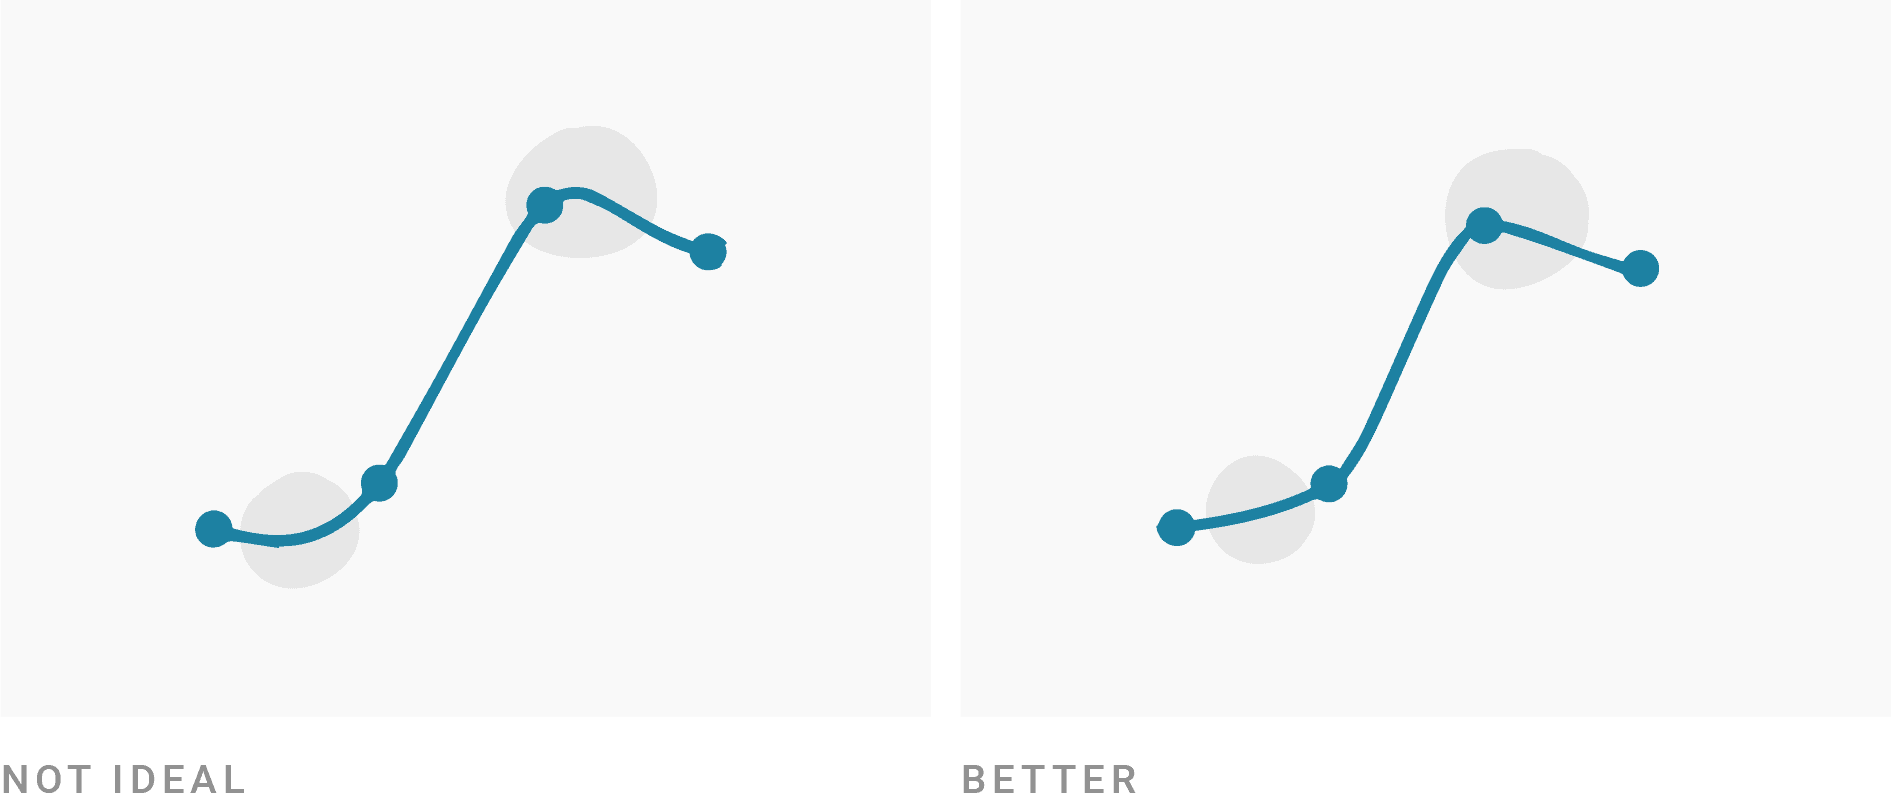
\includegraphics[width=\linewidth]{images/line-chart/line-chart-smoothing-caution.png}
        \fullwidthfigurecaption{Apply smoothing only when the underlying process is continuous; otherwise curves can invent turning points or distort local magnitude changes.}
        \label{fig:line-chart-smoothing-caution}
    \end{minipage}
\end{figure*}

\subsection{Idiom: Area Charts}
\paragraph{Brief}
An area chart (also called an area graph) extends a line chart by filling the region between the line and the baseline. This fill adds a stronger sense of magnitude and accumulated volume while still preserving trend reading along an ordered axis. With a single series, it emphasises magnitude over time; with multiple series, the areas should be stacked vertically rather than overlap, so the chart can still communicate both component evolution and total change.

% \begin{marginfigure}
%     \centering
%     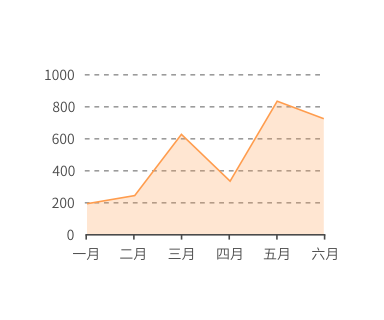
\includegraphics[width=\linewidth]{images/area-chart/area-chart-intro.png}
%     \caption{Basic area chart idiom.}
%     \label{fig:area-chart-intro}
% \end{marginfigure}

\whatpill\  An area chart uses one \textbf{ordered key attribute} (usually time) and one \textbf{quantitative value attribute}; multi-series area charts add one \textbf{categorical key attribute} and stack the series at each position.

\begin{figure*}[htbp]
    \centering
    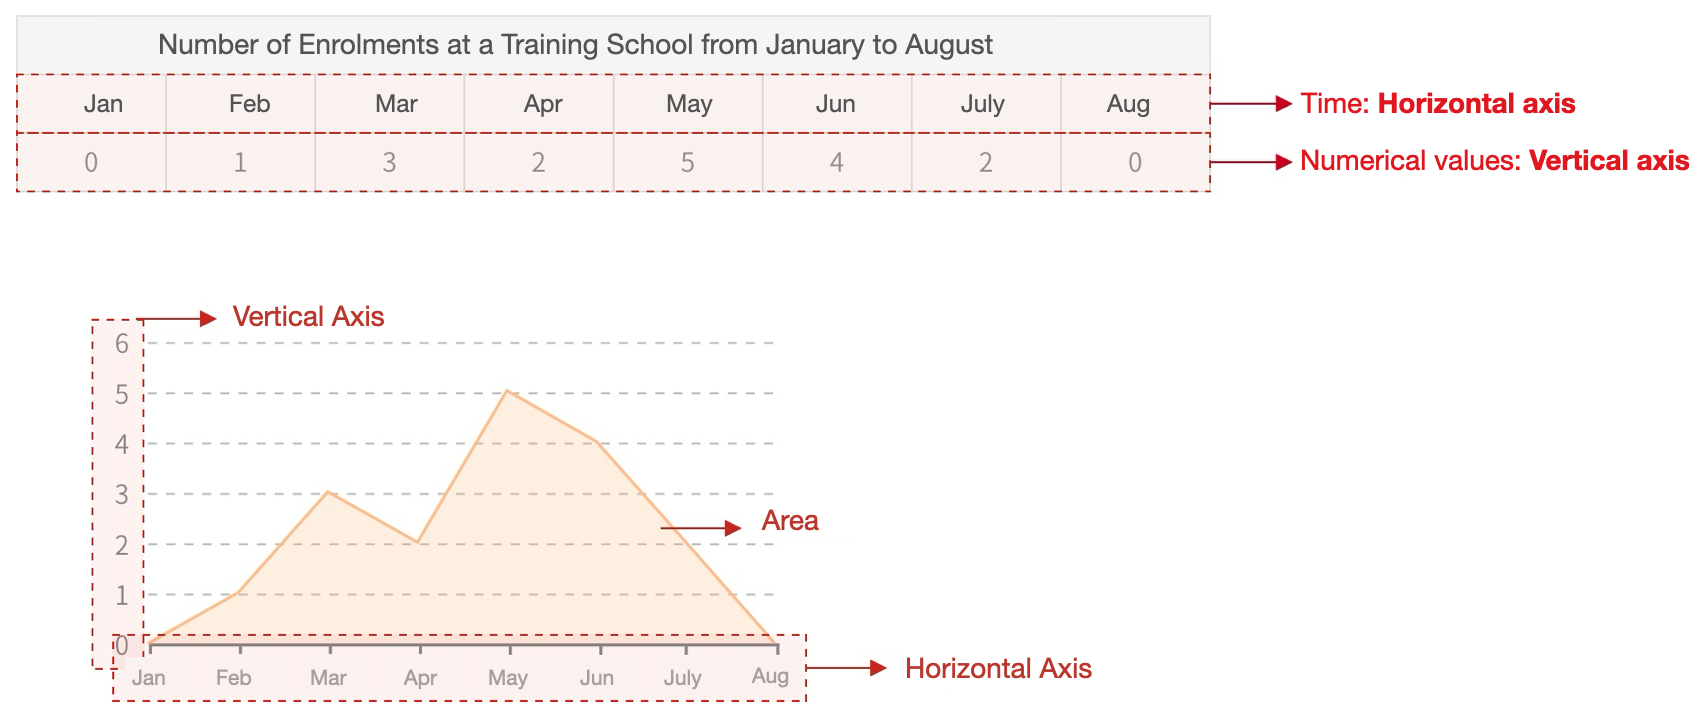
\includegraphics[width=0.92\linewidth]{images/area-chart/area-chart-elemental-composition.png}
    \caption{Elemental composition of a single-series area chart: ordered x-axis, quantitative y-axis, and filled region under the trend line.}
    \label{fig:area-chart-elemental-composition}
\end{figure*}

When an area chart expands from one filled series to multiple categories, the idiom changes from showing a single magnitude over time to showing composition and total together. At that point, the series should be stacked rather than overlaid, so readers can still interpret both the whole and its parts.

\begin{figure*}[htbp]
    \raggedright
    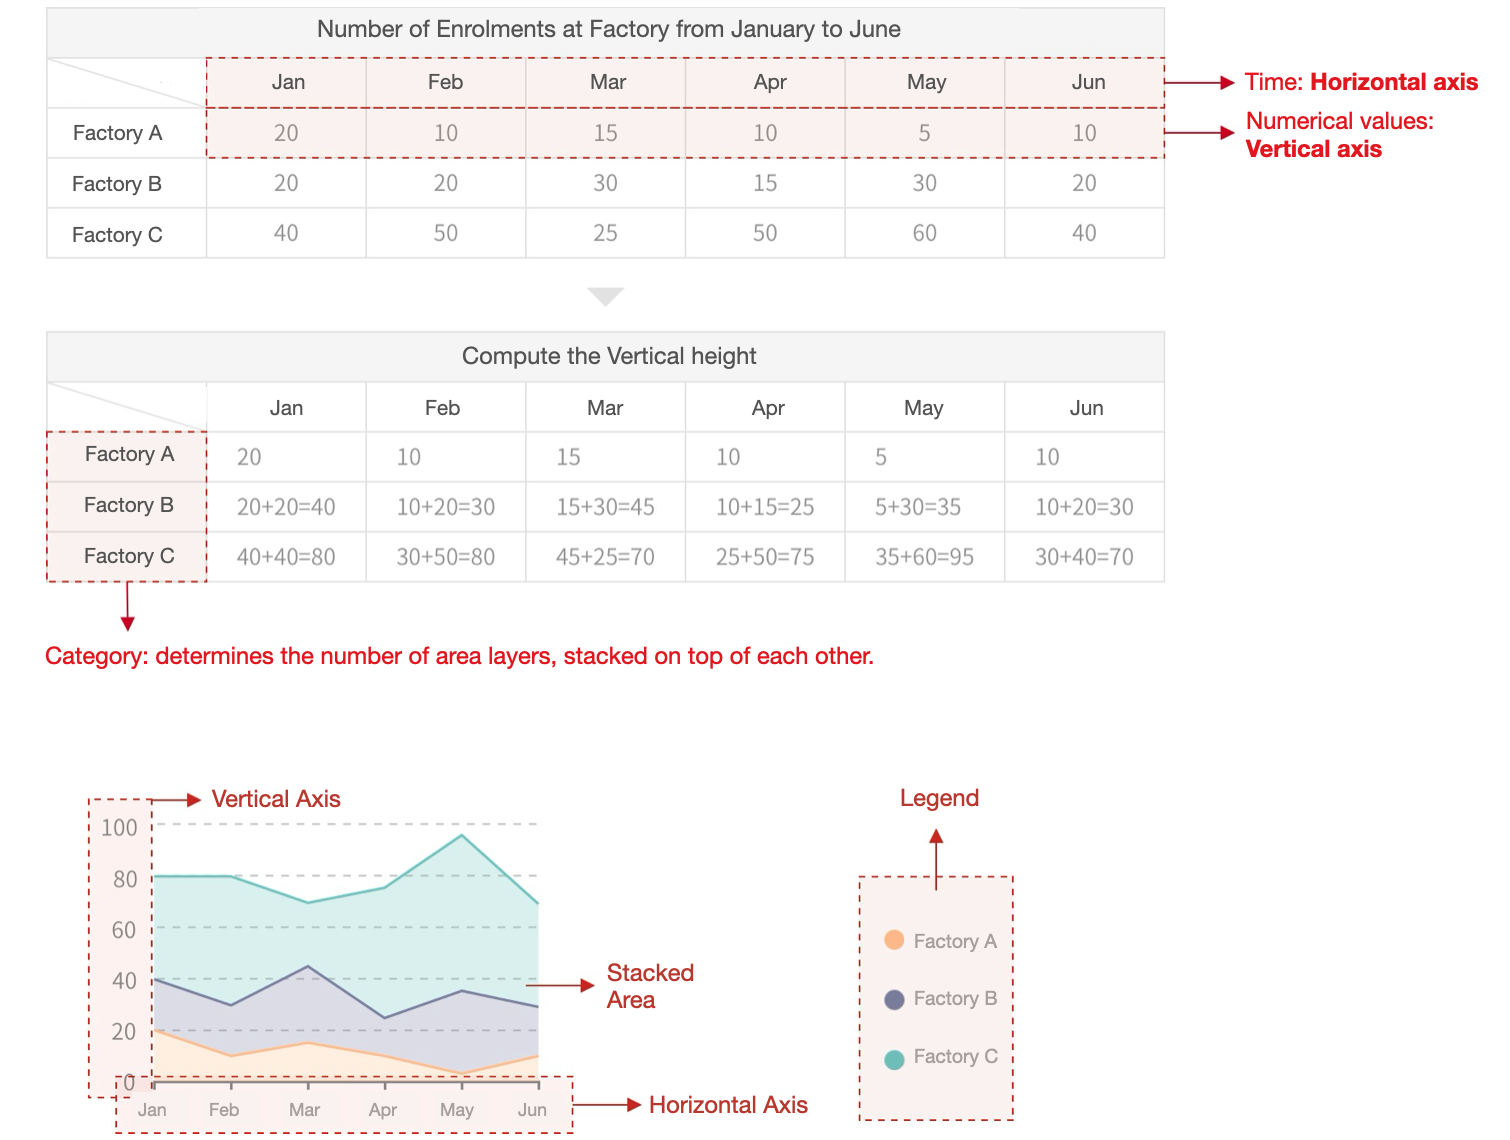
\includegraphics[width=\linewidth]{images/area-chart/stacked-area-chart-elemental-composition.png}
    \caption{Elemental composition of a multi-series area chart: once multiple filled series are shown together, they should be stacked to preserve totals and composition.}
    \label{fig:stacked-area-chart-elements}
\end{figure*}

\whypill\  The main \textit{task} is \textbf{analyse}, and the primary \textit{target} is \textbf{trend} over time. Secondary tasks are \textbf{query} of approximate magnitude, total growth, and composition change when multiple series are stacked.

\howpill\  At the \textbf{idiom} level, the \textit{mark} is \textbf{area} (filled polygon under a line). The primary \textit{channels} are \textbf{vertical position} of the boundary for value and optional \textbf{hue} for series identity. In multi-series cases, layer ordering matters because only the bottom layer keeps a stable baseline; \textbf{scalability} is therefore lower than line charts when many stacked layers are present.

\subsection*{Design Guide}
\margincitebox[Design Guidance Sources]{datawrapper_area_chart_guidance}
\paragraph{Use when}
\begin{itemize}
    \item \textit{Ordered time development.} Area charts should be used when the horizontal axis is truly ordered, especially temporal, and the goal is to show how values develop over time (see Figure~\ref{fig:area-chart-use-only-time}).
    \item \textit{Total and shares are both important.} Area charts are particularly useful when readers need to perceive overall total and internal composition simultaneously. If only share-to-share comparison matters, line charts are often clearer (see Figure~\ref{fig:area-chart-applicable-total-and-many-dates}).
    \item \textit{Single-series magnitude or few stacked components.} Area charts work best either for one series where filled magnitude matters, or for a small number of stacked components whose contributions are visibly substantial (see Figure~\ref{fig:stacked-area-chart-elements} and Figure~\ref{fig:area-chart-applicable-differences-and-multi}).
\end{itemize}

\begin{marginfigure}
    \centering
    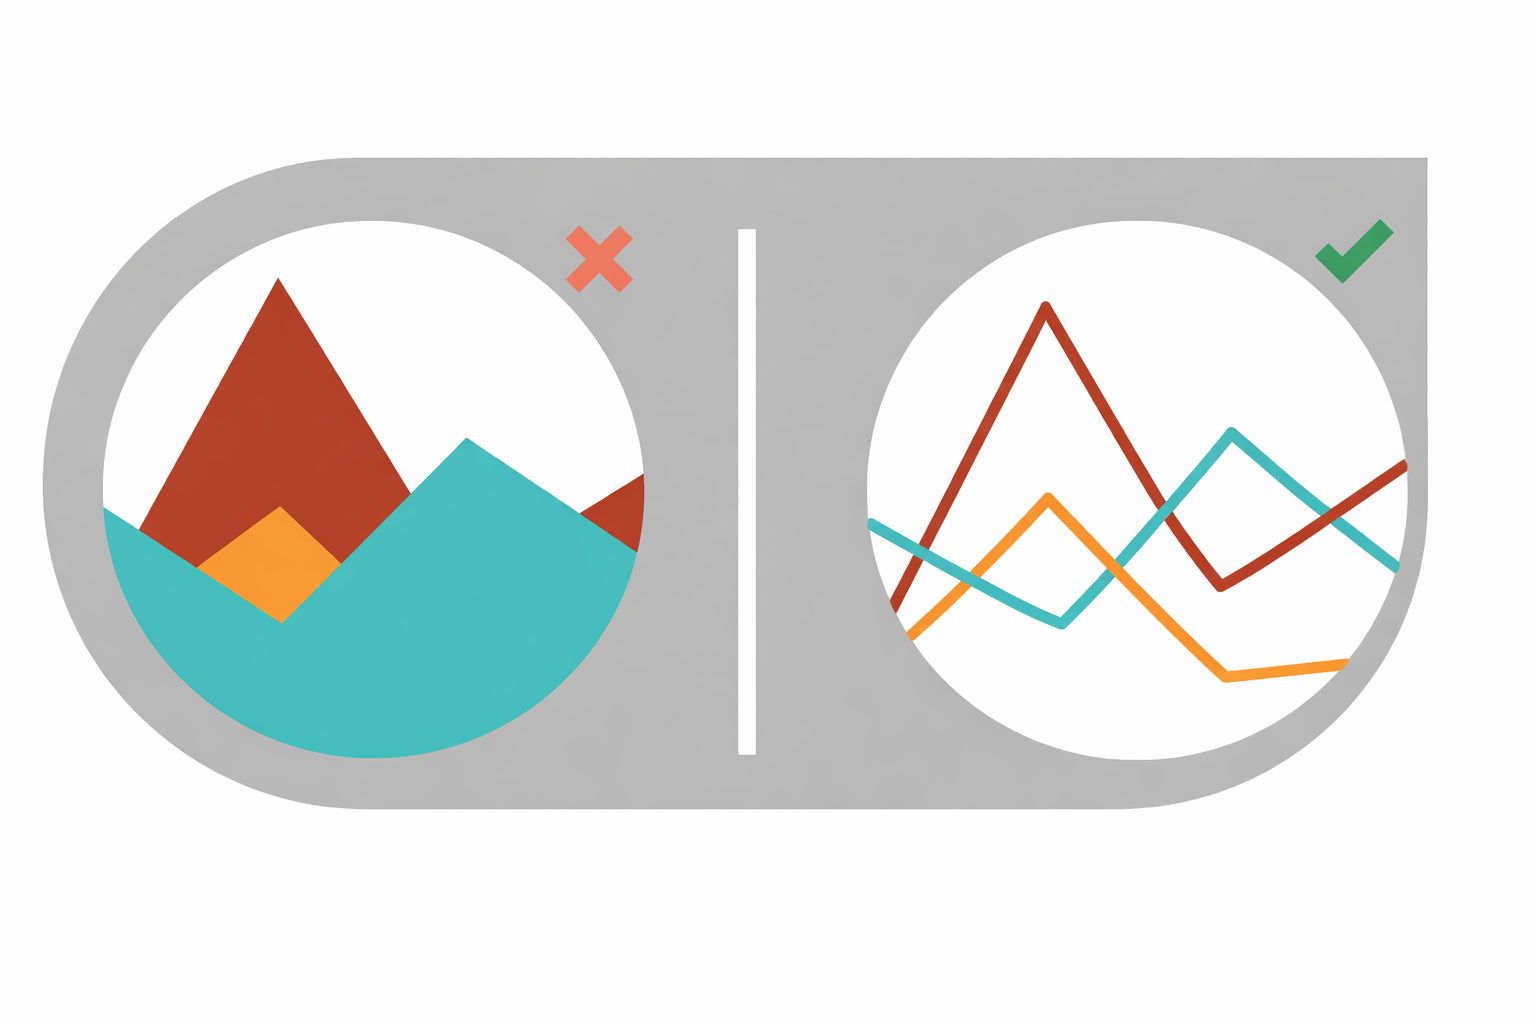
\includegraphics[width=\linewidth]{images/area-chart/area-chart-overlap.png}
    \caption{Inapplicable case: multiple filled series are overlaid, producing occlusion and ambiguous color mixing. Try line charts instead, or stack the areas if composition and totals are important.}
    \label{fig:area-chart-overlap-limit}
\end{marginfigure}

\paragraph{Avoid when}
\begin{itemize}
    \item \textit{Unordered categories on the x-axis.} If the horizontal axis contains nominal categories (for example, fruit types), area continuity implies a sequence that does not exist. In that case, bar charts are a better idiom for category comparison.
    \item \textit{Unstacked multi-series overlays.} If multiple filled series are drawn independently on top of each other, occlusion and color mixing make the chart difficult to interpret. Stack the areas or switch to line charts instead (see Figure~\ref{fig:area-chart-overlap-limit}).
    \item \textit{Precise share-to-share comparison or crossover stories.} Area charts are not ideal when the main goal is to compare two shares directly or detect one series overtaking another. Line charts usually make these comparisons clearer (see Figure~\ref{fig:area-chart-not-best-share-comparison}).
    \item \textit{Too many series or negative values.} Readability degrades quickly with many layers, and negative values are difficult to interpret in multi-series area charts.
    \item \textit{Alternative baseline needs in dense stories.} In some dense multi-series narratives, a streamgraph (centered, moving baseline) can distribute layers more evenly and improve readability.
\end{itemize}


%\paragraph{Wrap up}
%In summary, area charts can communicate trend and magnitude well, but only when order, layering, and comparison goals are explicit. The key refinement suggestions are:

\paragraph{Refinements}
\begin{figure*}[htbp]
    \centering
    \begin{minipage}[t]{0.48\linewidth}
        \centering
        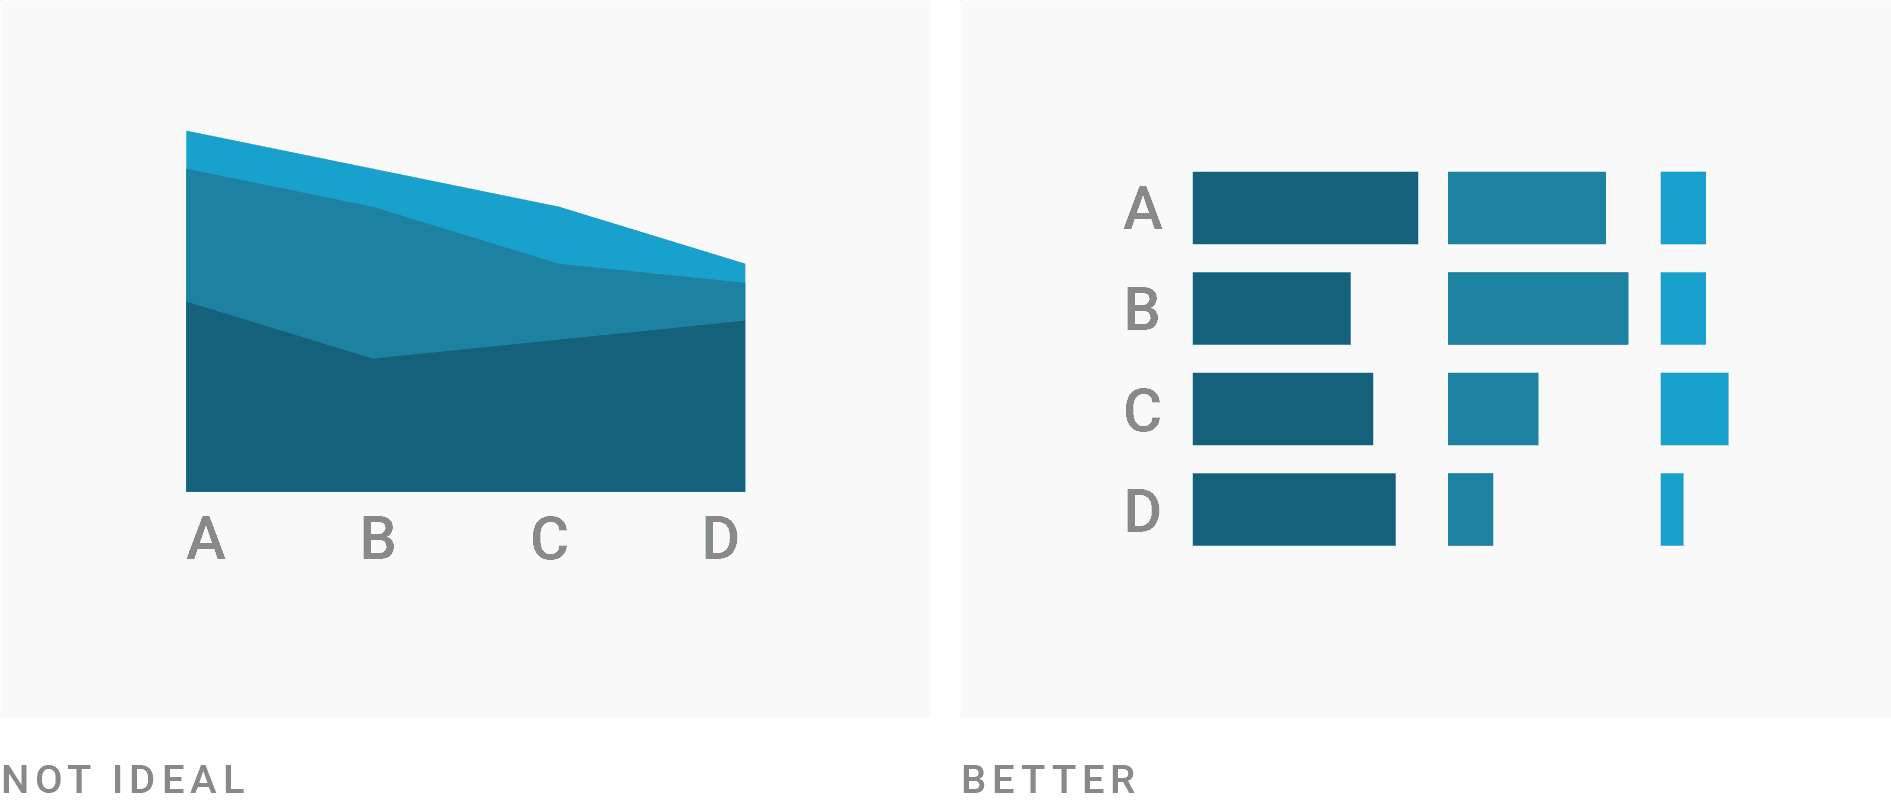
\includegraphics[width=\linewidth]{images/area-chart/area-chart-use-only-for-time.png}
        \fullwidthfigurecaption{Use area charts only with a truly ordered axis (typically time); for unordered categories, bar-based layouts communicate comparisons more faithfully.}
        \label{fig:area-chart-guidance-a}
        \label{fig:area-chart-use-only-time}
    \end{minipage}
    \hfill
    \begin{minipage}[t]{0.48\linewidth}
        \centering
        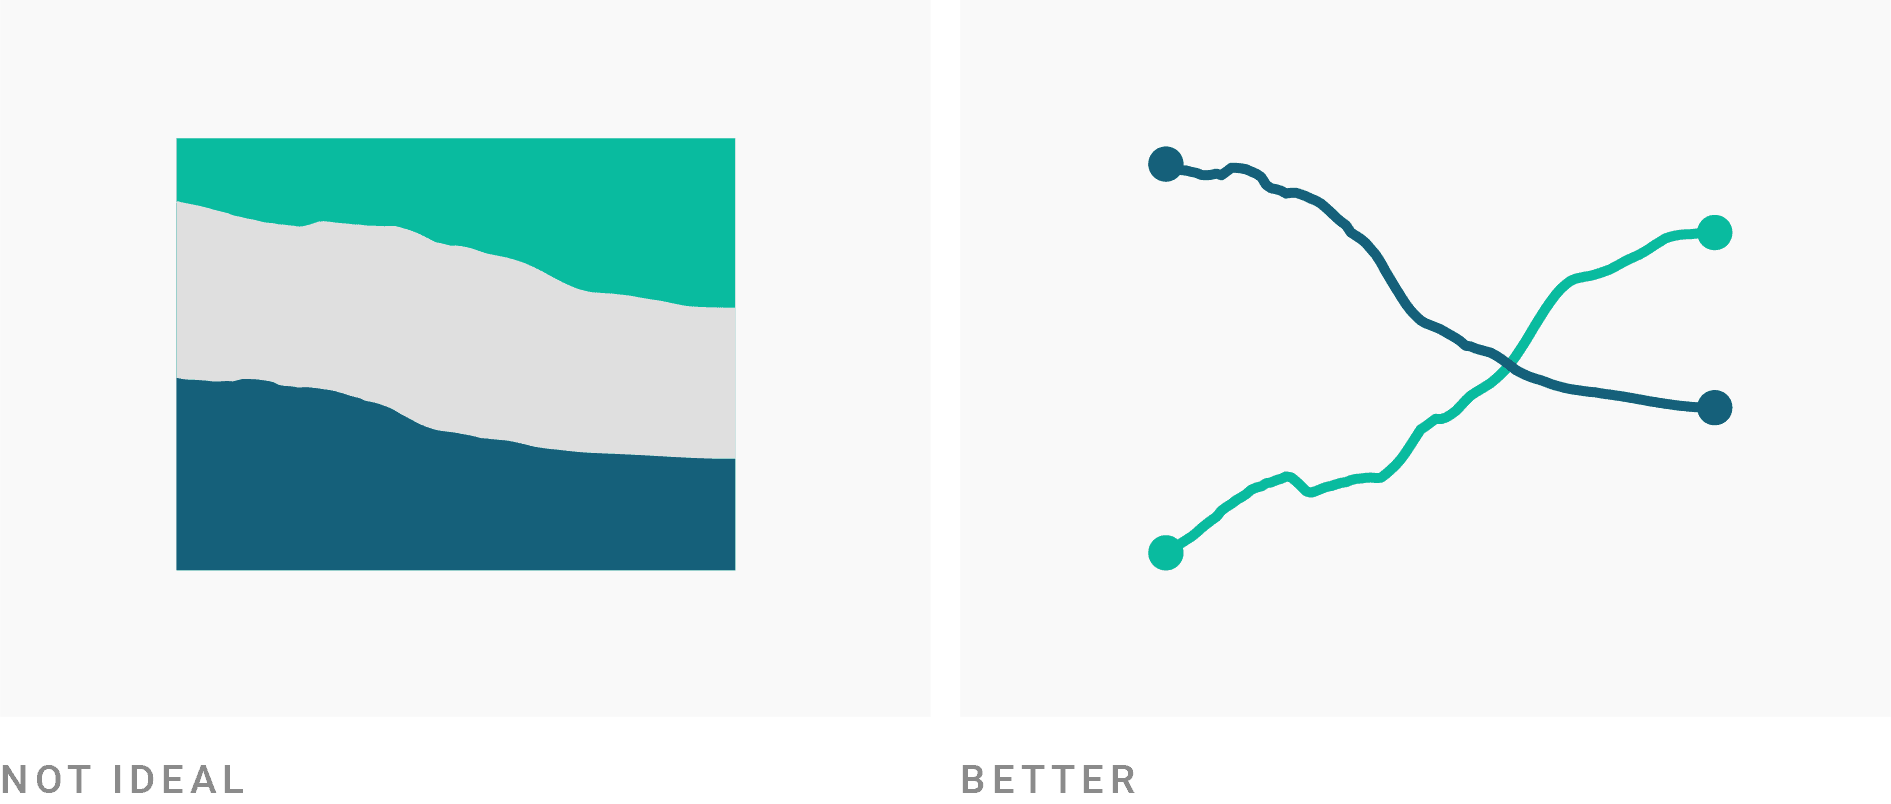
\includegraphics[width=\linewidth]{images/area-chart/area-chart-not-best-for-share-comparison.png}
        \fullwidthfigurecaption{For precise share-to-share comparison or overtaking stories, line charts are clearer because aligned baselines are easier to compare than stacked fills.}
        \label{fig:area-chart-not-best-share-comparison}
    \end{minipage}
\end{figure*}

\begin{figure*}[htbp]
    \centering
    \begin{minipage}[t]{0.48\linewidth}
        \centering
        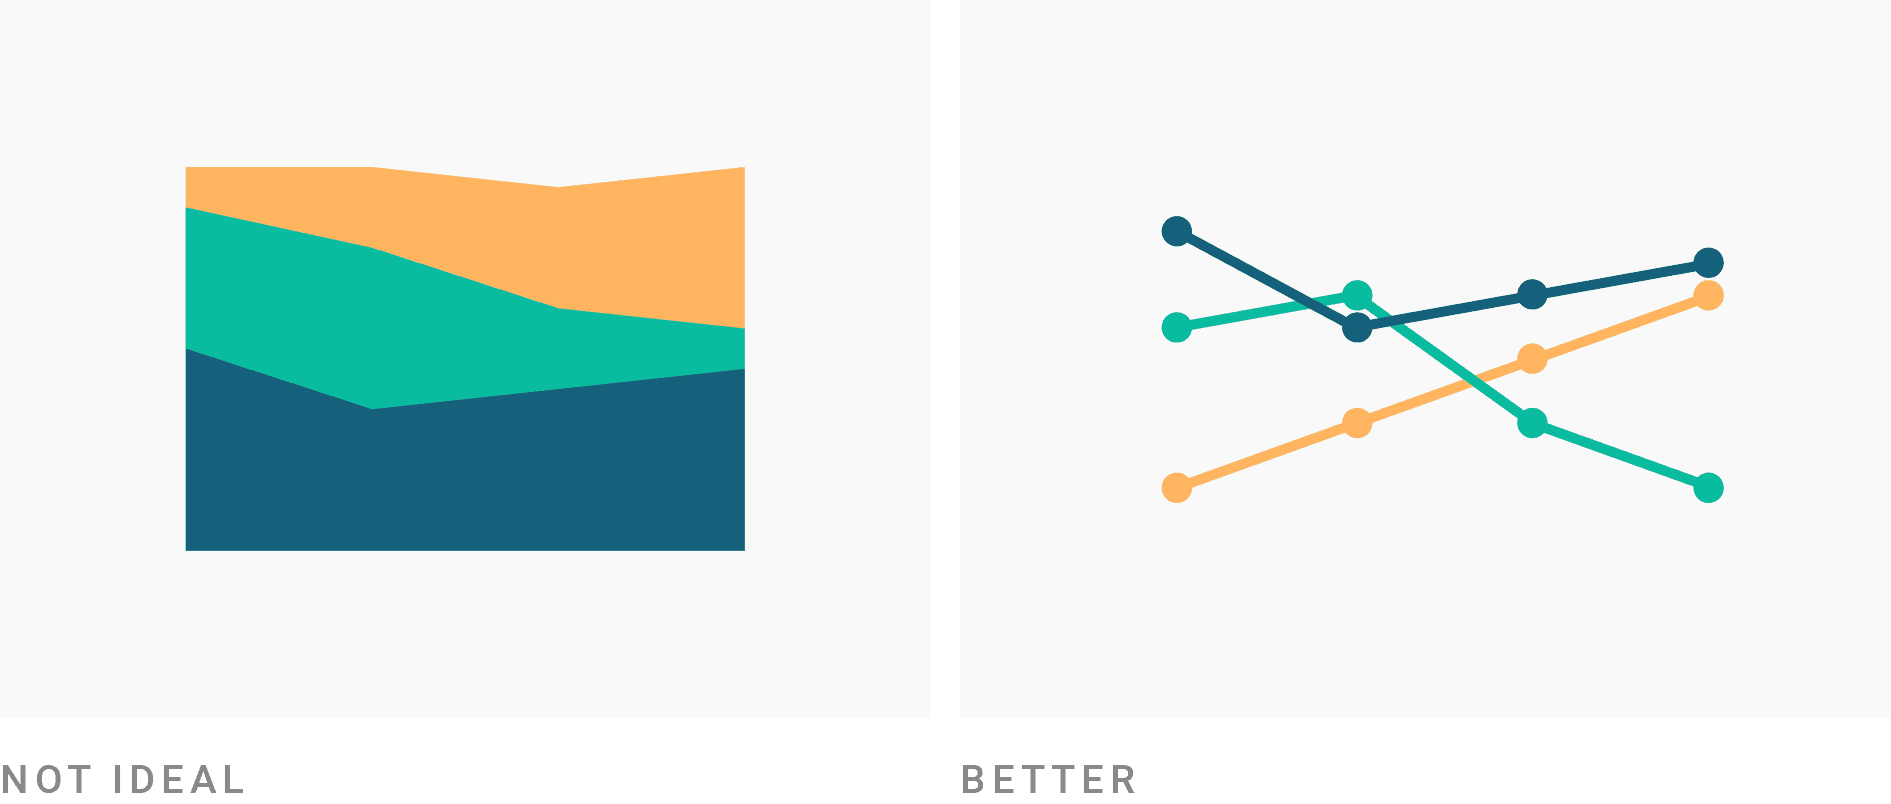
\includegraphics[width=\linewidth]{images/area-chart/area-chart-total-and-shares-important.png}
        \fullwidthfigurecaption{Choose area charts when both total magnitude and composition over time are important, not when component trends are the only goal.}
        \label{fig:area-chart-guidance-b}
        \label{fig:area-chart-applicable-total-and-many-dates}
    \end{minipage}
    \hfill
    \begin{minipage}[t]{0.48\linewidth}
        \centering
        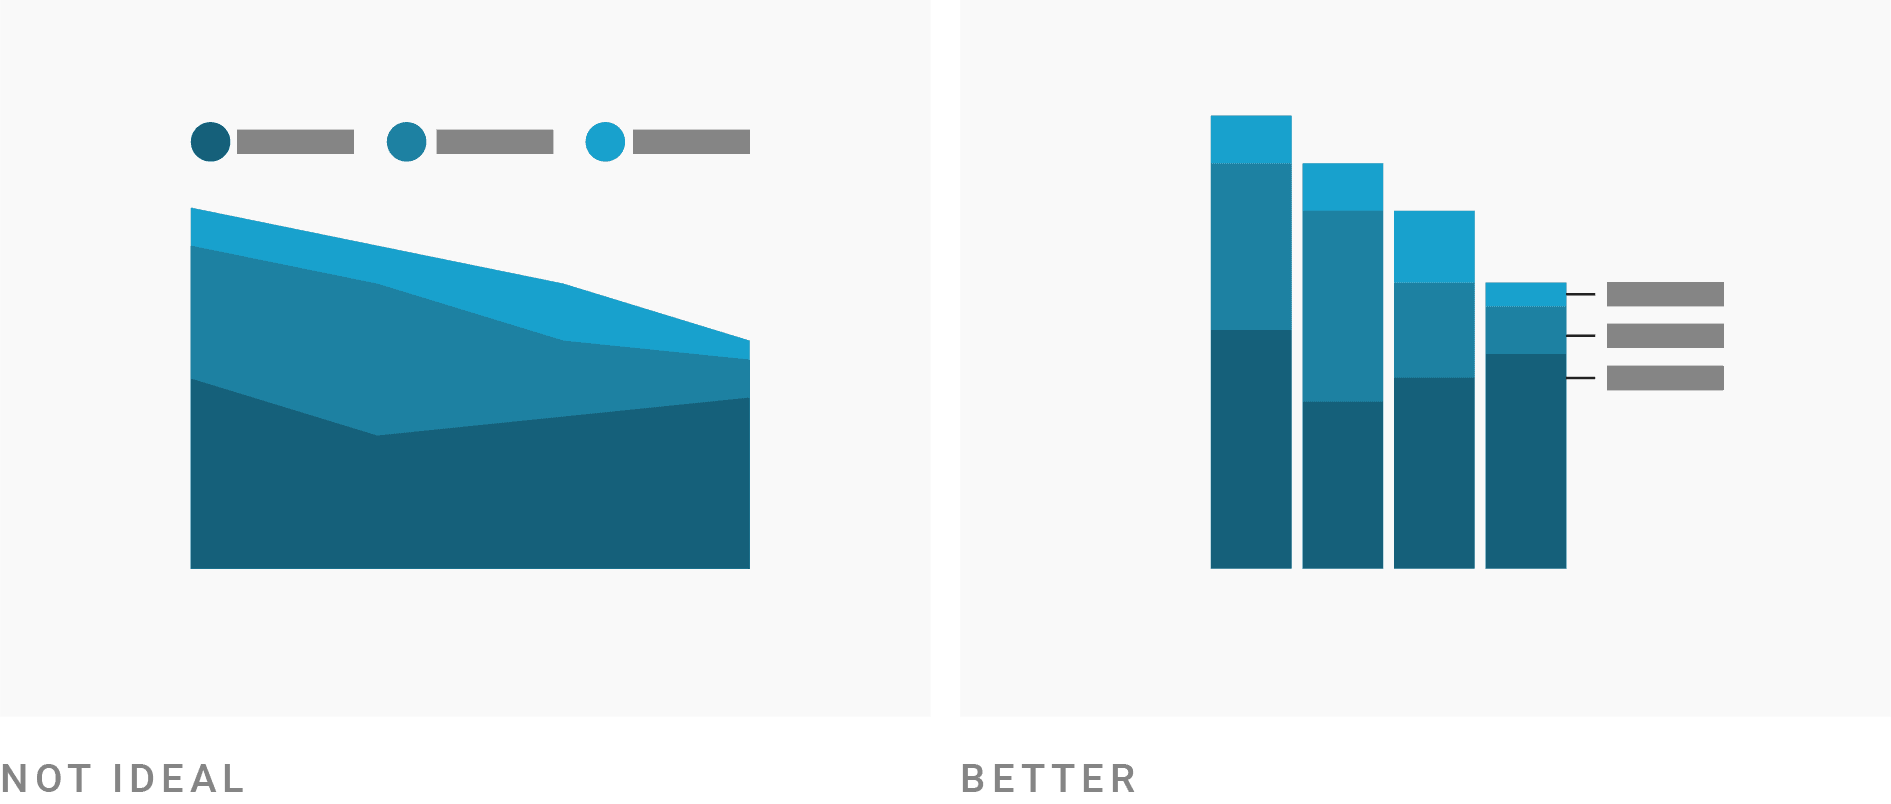
\includegraphics[width=\linewidth]{images/area-chart/area-chart-many-dates-better.png}
        \fullwidthfigurecaption{Area charts are often more effective with many dates; with only a few time points, stacked columns can provide clearer part comparison and labeling.}
        \label{fig:area-chart-guidance-b-many-dates}
    \end{minipage}
\end{figure*}

\begin{figure*}[htbp]
    \centering
    \begin{minipage}[t]{0.48\linewidth}
        \centering
        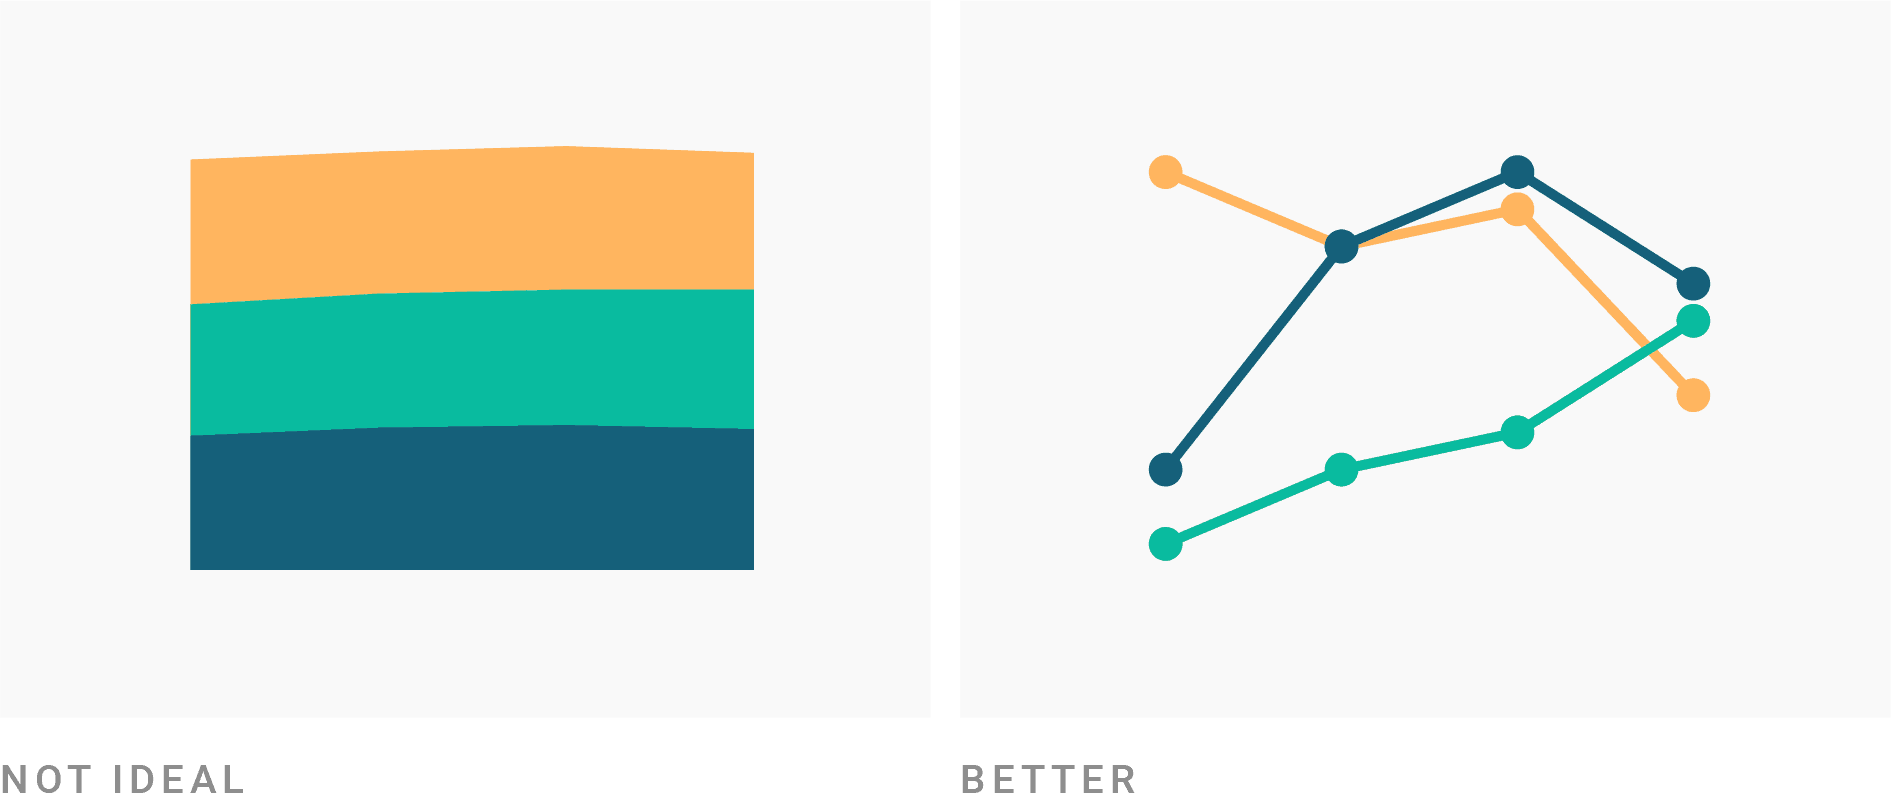
\includegraphics[width=\linewidth]{images/area-chart/area-chart-large-differences-better.png}
        \fullwidthfigurecaption{Filled areas are easier to read when differences between stacked series are substantial; very small gaps are usually clearer in line charts with focused scales.}
        \label{fig:area-chart-guidance-c}
        \label{fig:area-chart-applicable-differences-and-multi}
    \end{minipage}
    \hfill
    \begin{minipage}[t]{0.48\linewidth}
        \centering
        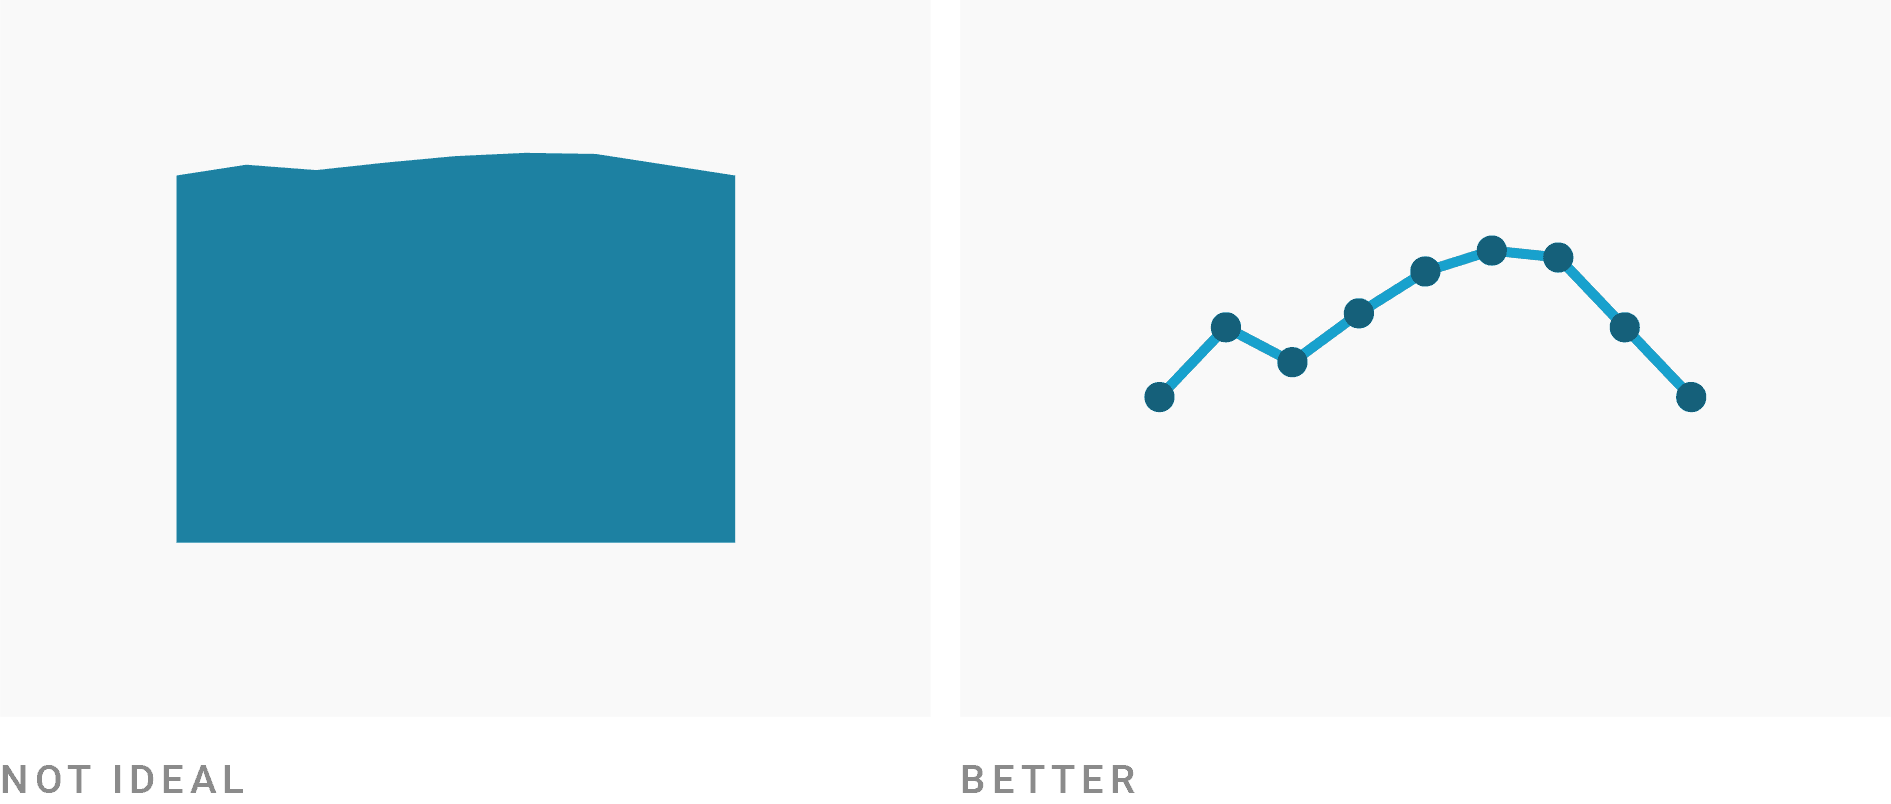
\includegraphics[width=\linewidth]{images/area-chart/area-chart-multiple-values-over-time.png}
        \fullwidthfigurecaption{Area charts can compare multiple temporal series in one view, but only when the series are stacked, layering remains legible, and category count is controlled.}
        \label{fig:area-chart-guidance-c-multiple-values}
    \end{minipage}
\end{figure*}

\begin{figure*}[htbp]
    \centering
    \begin{minipage}[t]{0.48\linewidth}
        \centering
        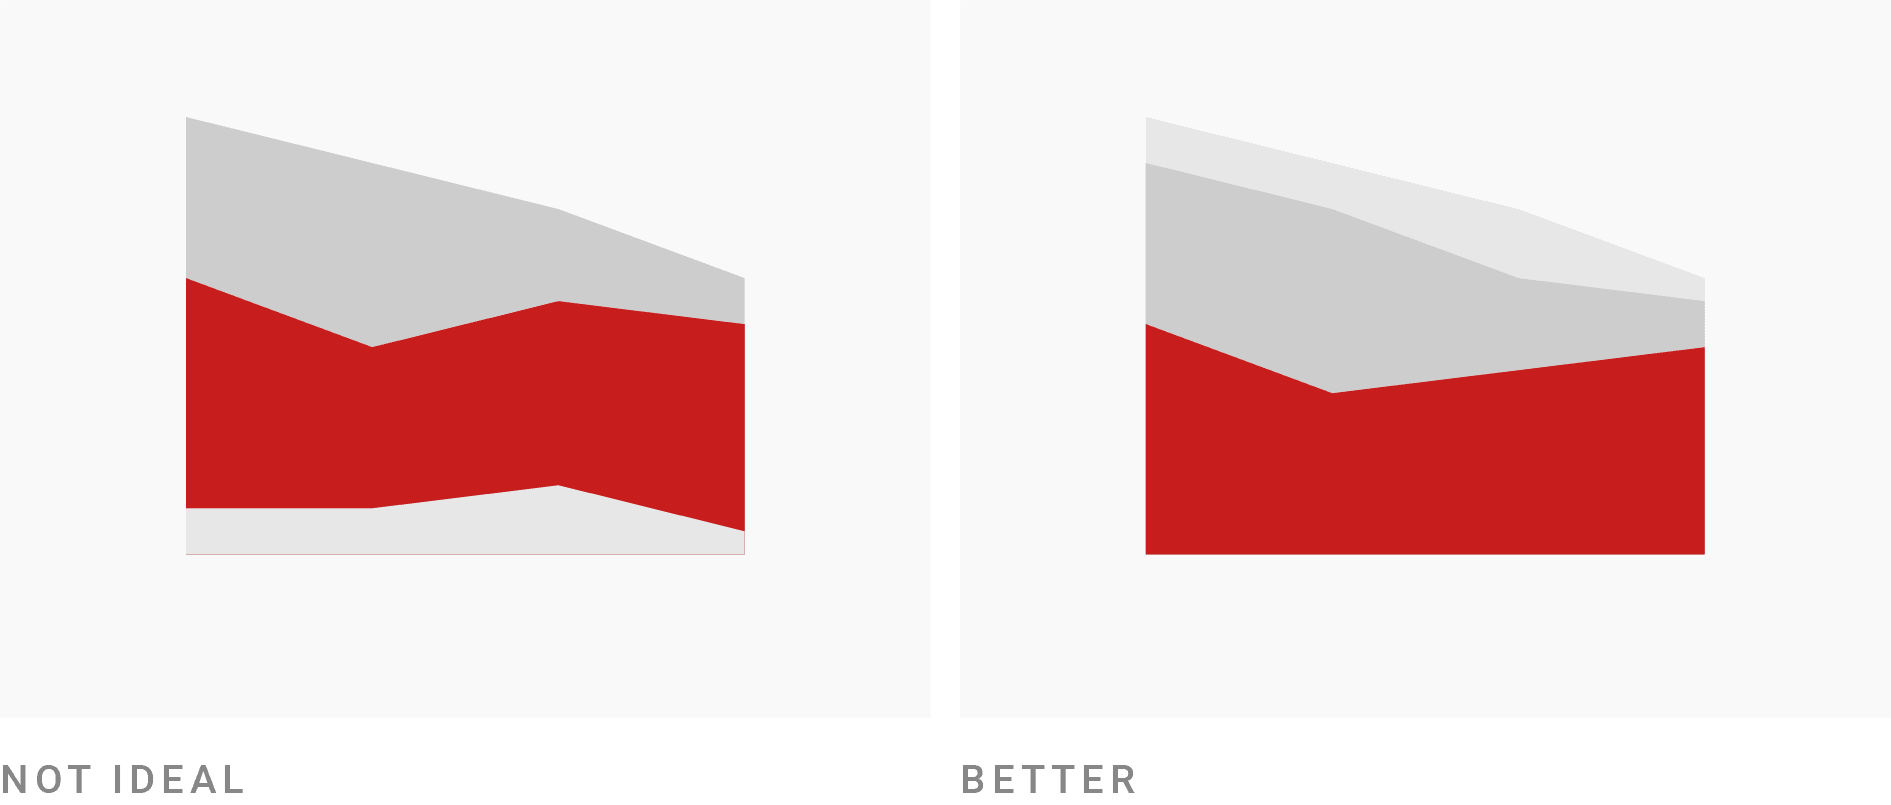
\includegraphics[width=\linewidth]{images/area-chart/area-chart-important-series-at-bottom.png}
        \fullwidthfigurecaption{Place important series near the baseline so they retain a stable reference for comparison, and use stronger color emphasis for the priority layer.}
        \label{fig:area-chart-design-guidance-a}
        \label{fig:area-chart-design-guidance-a-important-bottom}
    \end{minipage}
    \hfill
    \begin{minipage}[t]{0.48\linewidth}
        \centering
        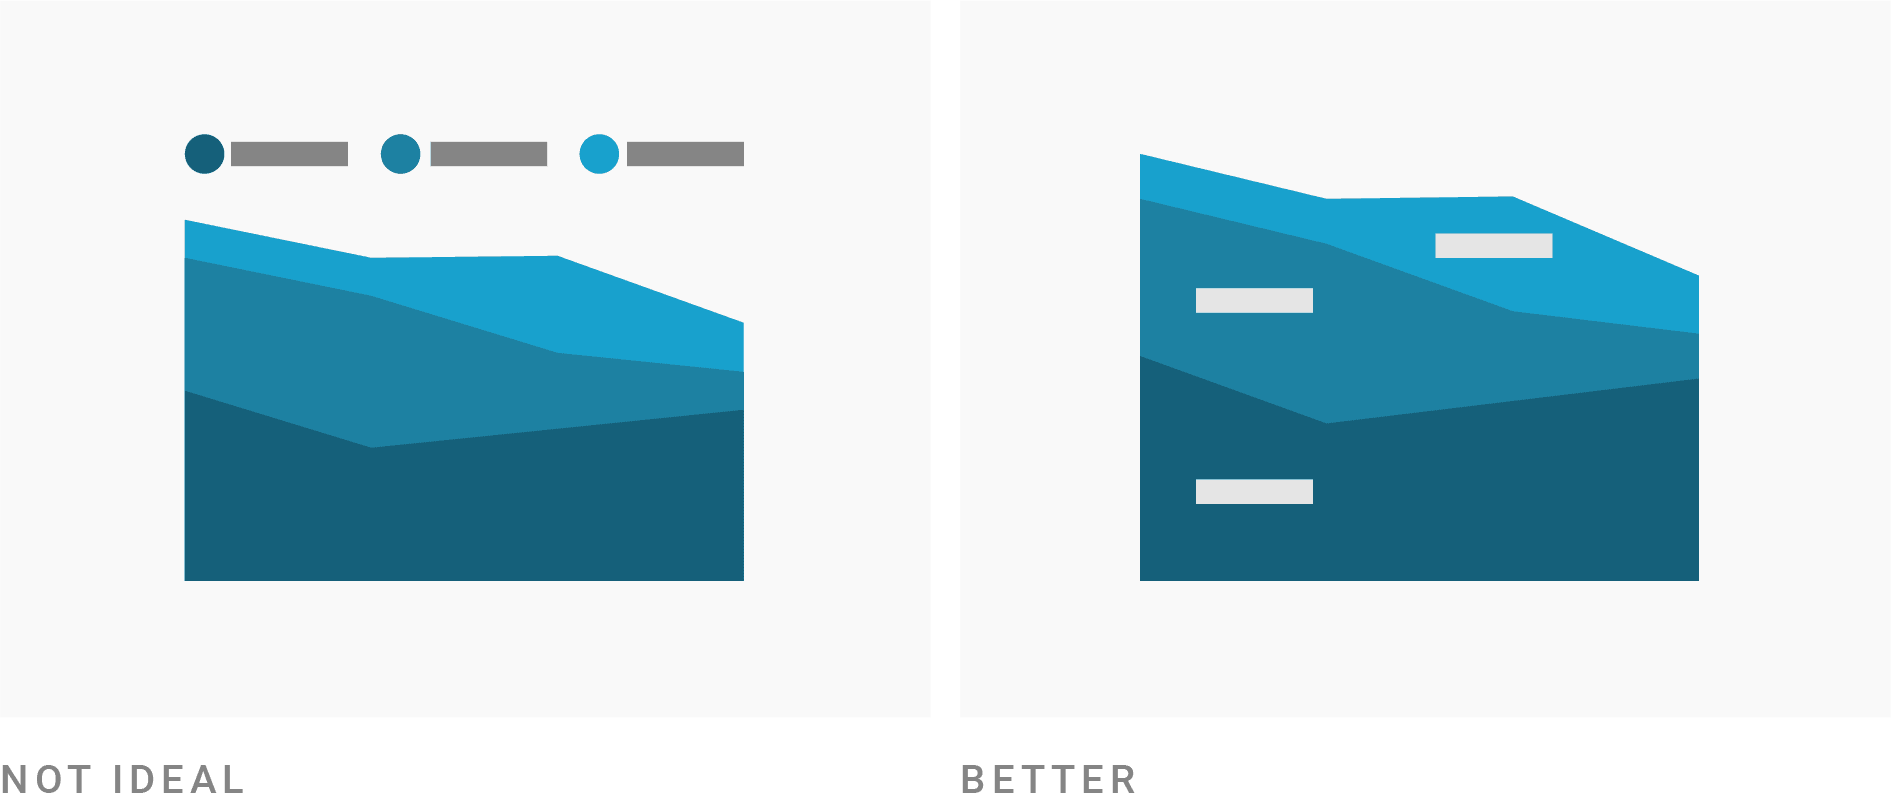
\includegraphics[width=\linewidth]{images/area-chart/area-chart-direct-labeling.png}
        \fullwidthfigurecaption{Use direct labels when space allows so readers can identify layers without repeatedly matching legend colors.}
        \label{fig:area-chart-design-guidance-a-direct-labeling}
    \end{minipage}
\end{figure*}

\begin{figure*}[htbp]
    \centering
    \begin{minipage}[t]{0.48\linewidth}
        \centering
        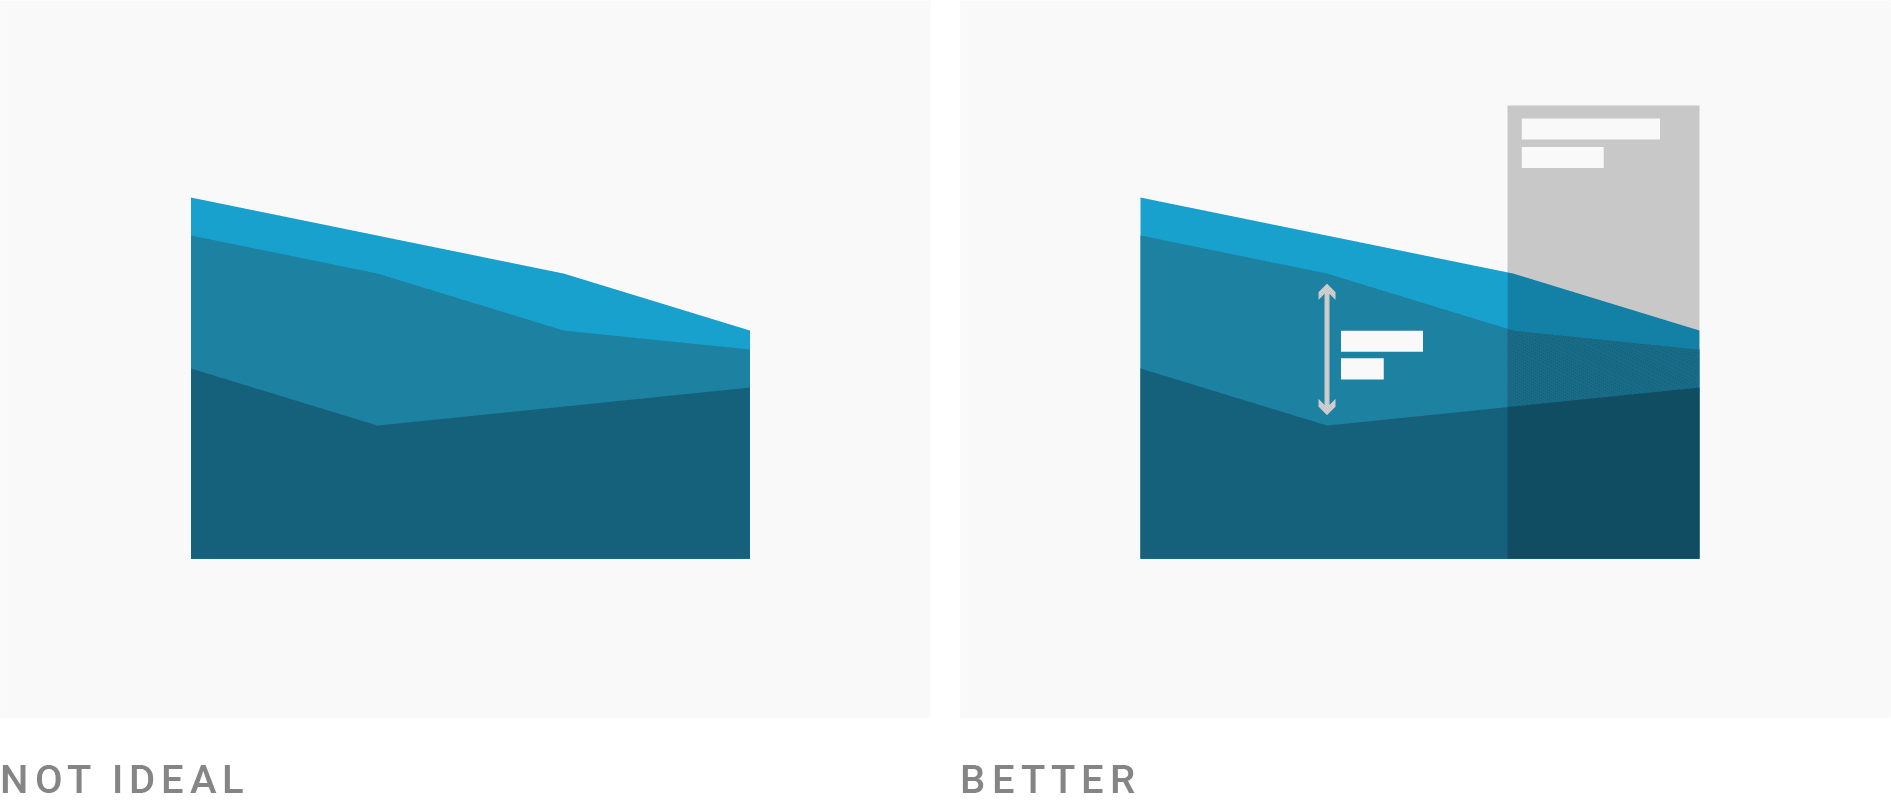
\includegraphics[width=\linewidth]{images/area-chart/area-chart-annotations-highlight-ranges.png}
        \fullwidthfigurecaption{Add annotations and highlighted ranges to mark regime shifts, policy changes, or external events that explain structural changes in layered areas.}
        \label{fig:area-chart-annotations-highlight-ranges}
    \end{minipage}
    \hfill
    \begin{minipage}[t]{0.48\linewidth}
        \centering
        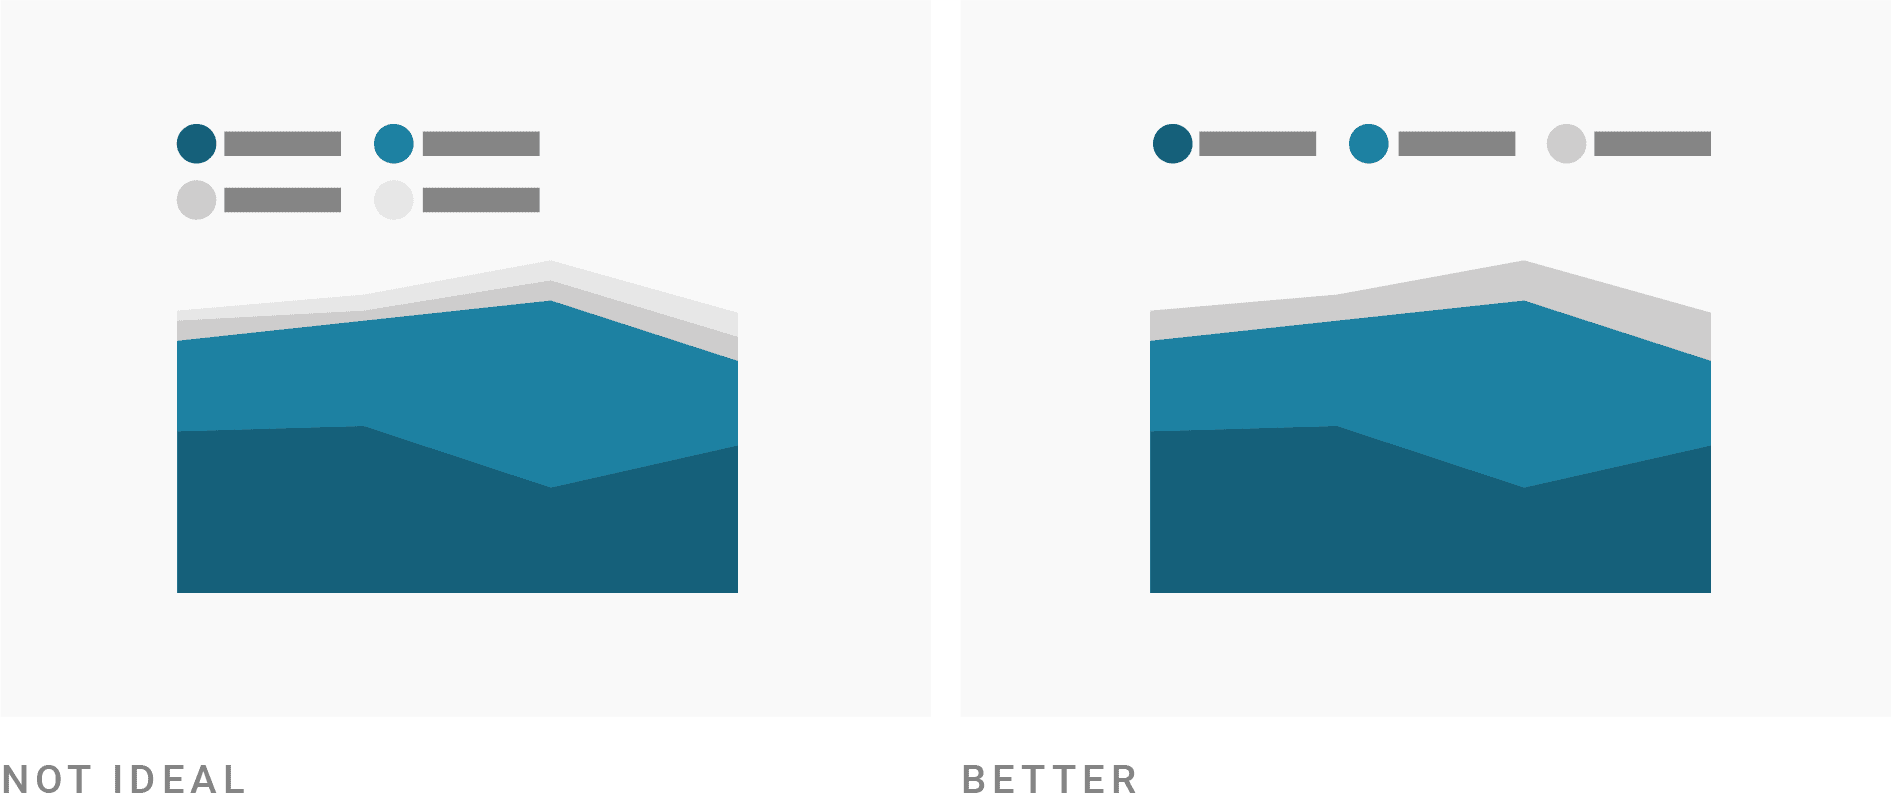
\includegraphics[width=\linewidth]{images/area-chart/area-chart-group-small-values.png}
        \fullwidthfigurecaption{Group tiny layers into ``Others'' to reduce visual noise and label overload, preserving attention on the dominant components.}
        \label{fig:area-chart-group-small-values}
    \end{minipage}
\end{figure*}

\subsection{Idiom: Pie Charts}
\paragraph{Brief}
A pie chart divides one whole into sectors and encodes each category as a share of 100\%. It is a composition idiom for part-to-whole reading, not a general-purpose comparison chart.
\margincitebox[Pie Chart References]{schwabish2021,datawrapper_pie_chart_guidance}

\whatpill\  A pie chart requires one \textbf{categorical key attribute} and one \textbf{quantitative value attribute} for a \textbf{single whole}. Categories should be mutually exclusive and collectively exhaustive, and values should sum to one denominator (typically 100\%).

\begin{figure*}[htbp]
    \raggedright
    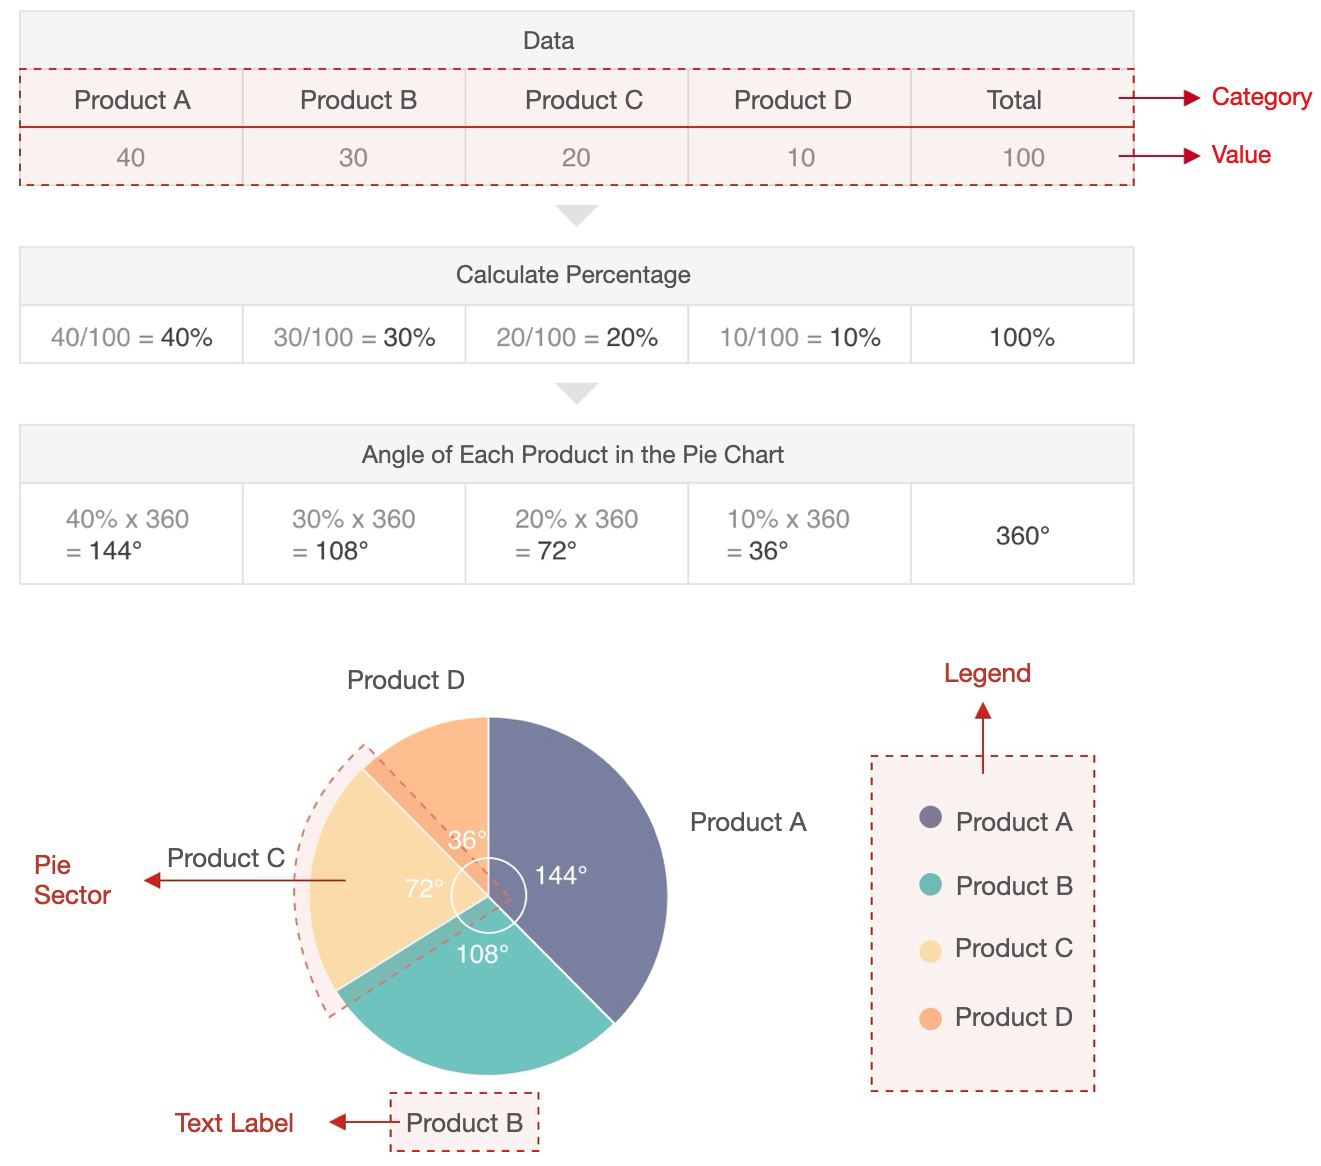
\includegraphics[width=0.8\linewidth]{images/pie-chart/pie-chart-elemental-composition.png}
    \caption{Elemental composition of a pie chart: sector angle/area encodes part-to-whole proportion.}
    \label{fig:pie-chart-elemental-composition}
\end{figure*}

\whypill\  The main \textit{task} is \textbf{query}, and the primary \textit{target} is a broad \textbf{part-to-whole relationship}: identify dominant shares and overall balance. Precision \textit{targets} (fine ranking or close-value comparison) are weak for this idiom.

\howpill\  At the \textbf{idiom} level, the \textit{mark} is \textbf{area} (circular sector). Relative quantity is encoded by \textbf{angle}/\textbf{arc}/\textbf{area} cues. \textbf{Scalability} is very limited: more than 5--6 categories usually reduce readability, and small shares are hard to label legibly.

\subsection*{Design Guide}
\margincitebox[Design Guidance Sources]{datawrapper_pie_chart_guidance}
\paragraph{Use when}
\begin{itemize}
    \item \textit{One total, few categories, clear differences.} Pie charts are suitable when composition is the message, category count is limited, and differences are visually clear.
    \item \textit{Space-constrained composition display.} Because pie charts keep a fixed circular footprint, they can be useful when we need a compact composition display in a constrained layout.
\end{itemize}

\paragraph{Avoid when}
\begin{itemize}
    \item \textit{Categories do not form a whole, or trend is the target.} Pie charts should not be used for unrelated categories or temporal trend analysis.
    \item \textit{Fine comparison between similar values.} Human perception compares aligned lengths more accurately than angles/areas \parencite{heer2010}. When values are close, bar charts are usually clearer, and pie charts are not ideal for precise share comparison (see Figure~\ref{fig:pie-chart-inapplicable-close-values}).
    \item \textit{Too many categories, or too little information.} Many slices reduce legibility and labeling quality; with only two values, a direct textual percentage can be clearer than a full pie chart (see Figure~\ref{fig:pie-chart-inapplicable-too-many-or-too-few}).
    \item \textit{Comparing multiple totals.} One pie chart can only show one total and its shares. If we need to compare two or more totals, stacked bars/columns are usually more effective.
\end{itemize}

%\paragraph{Wrap up}
%In summary, pie charts can work for compact part-to-whole stories, but they need strict control of category count and labeling. The key refinement suggestions are: 

\paragraph{Refinements}
\begin{figure*}[htbp]
    \centering
    \begin{minipage}[t]{0.48\linewidth}
        \centering
        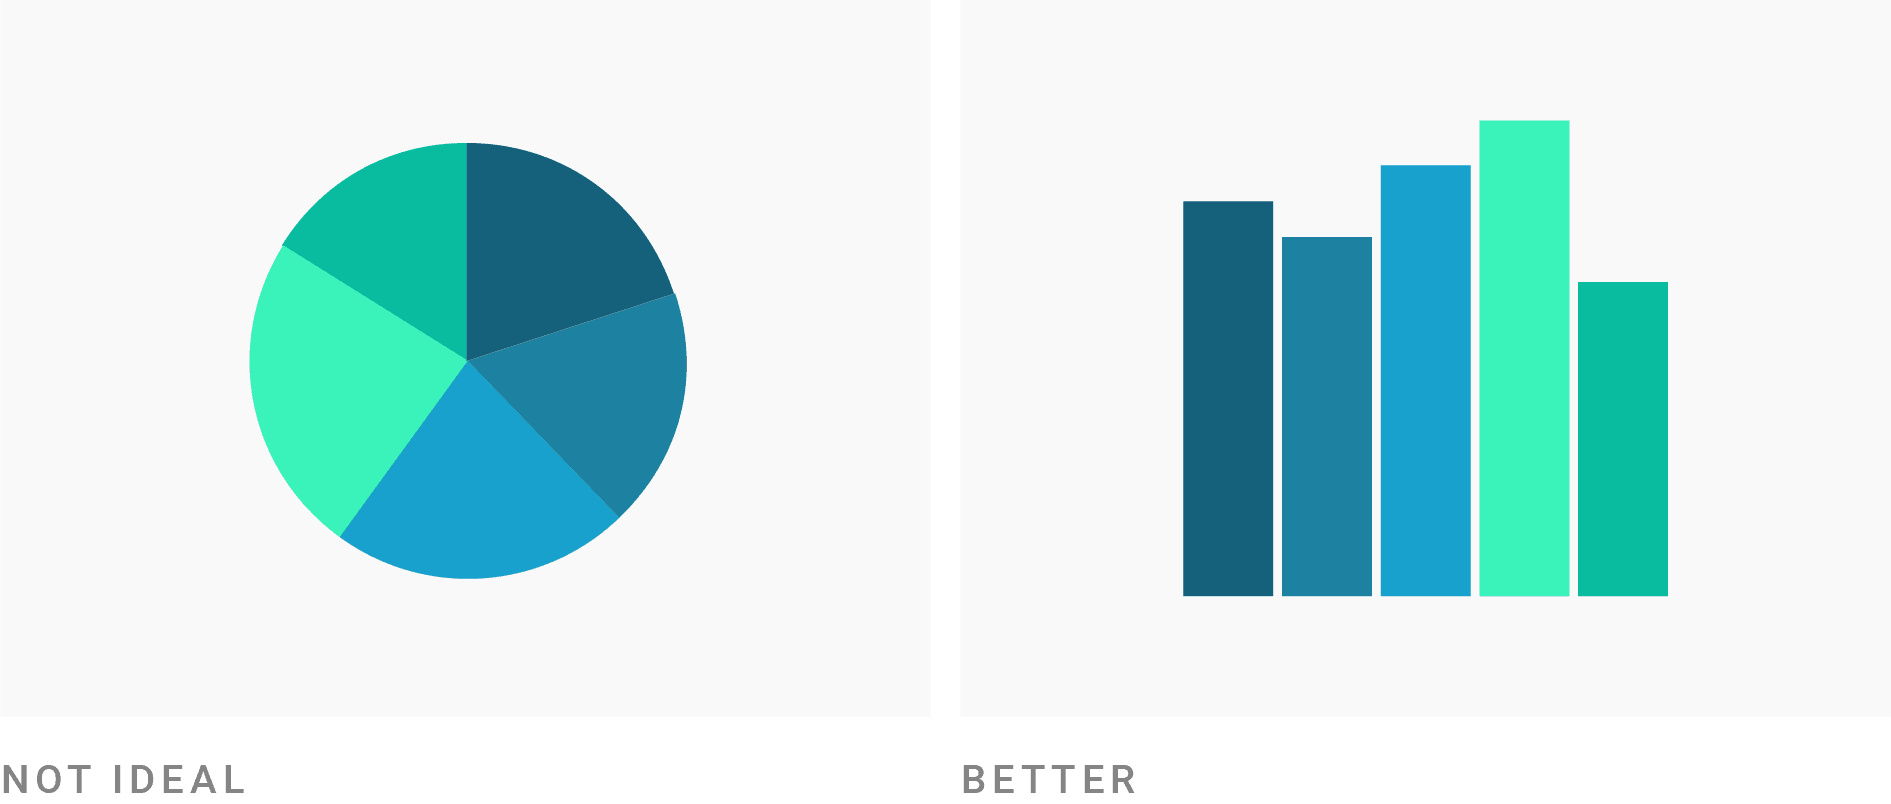
\includegraphics[width=\linewidth]{images/pie-chart/pie-chart-not-best-for-share-comparison.png}
        \fullwidthfigurecaption{Pie-chart limitation: similar shares are hard to compare precisely with angle/area encodings; use bars or dots when fine comparison is primary.}
        \label{fig:pie-chart-inapplicable-close-values}
    \end{minipage}
    \hfill
    \begin{minipage}[t]{0.48\linewidth}
        \centering
        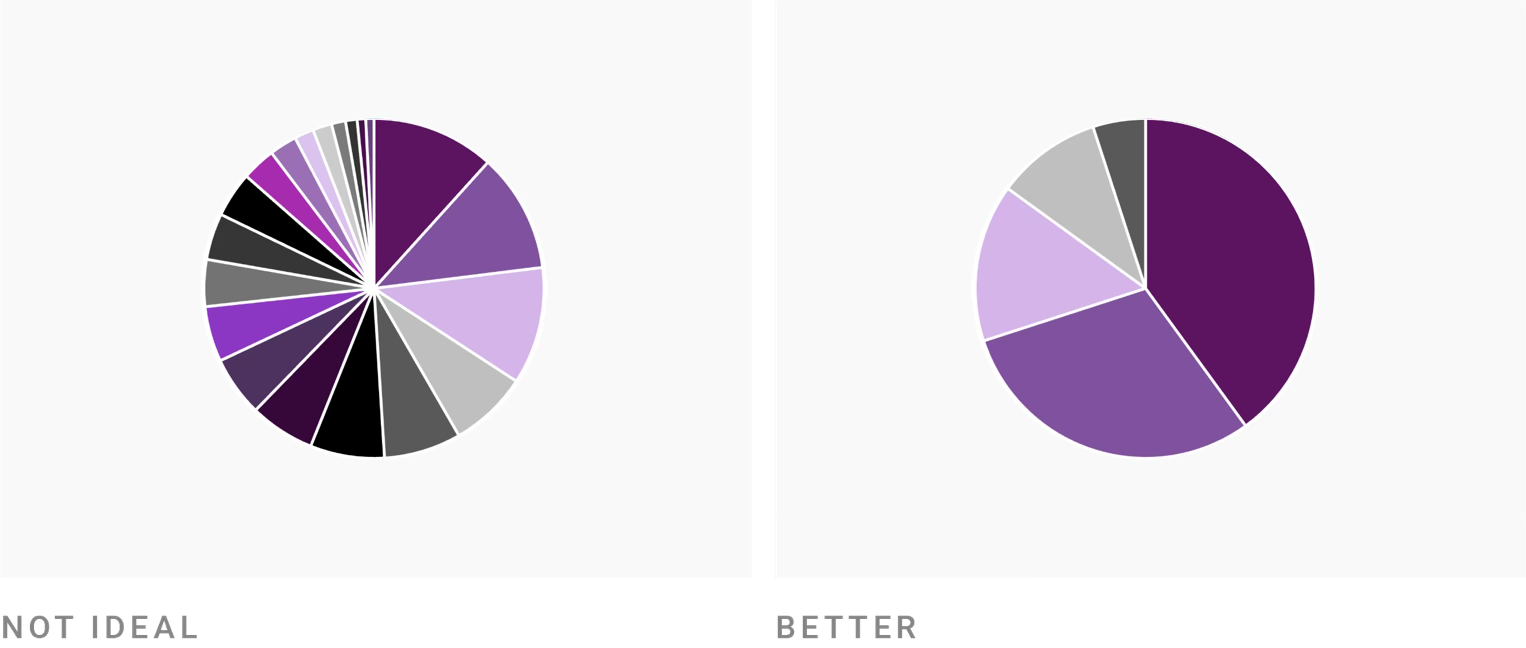
\includegraphics[width=\linewidth]{images/pie-chart/pie-chart-inapplicable-too-many-categories.png}
        \fullwidthfigurecaption{Pie-chart limitations: too many categories reduce readability.}
        \label{fig:pie-chart-inapplicable-too-many-or-too-few}
    \end{minipage}
\end{figure*}

\begin{figure*}[htbp]
    \centering
    \begin{minipage}[t]{0.48\linewidth}
        \centering
        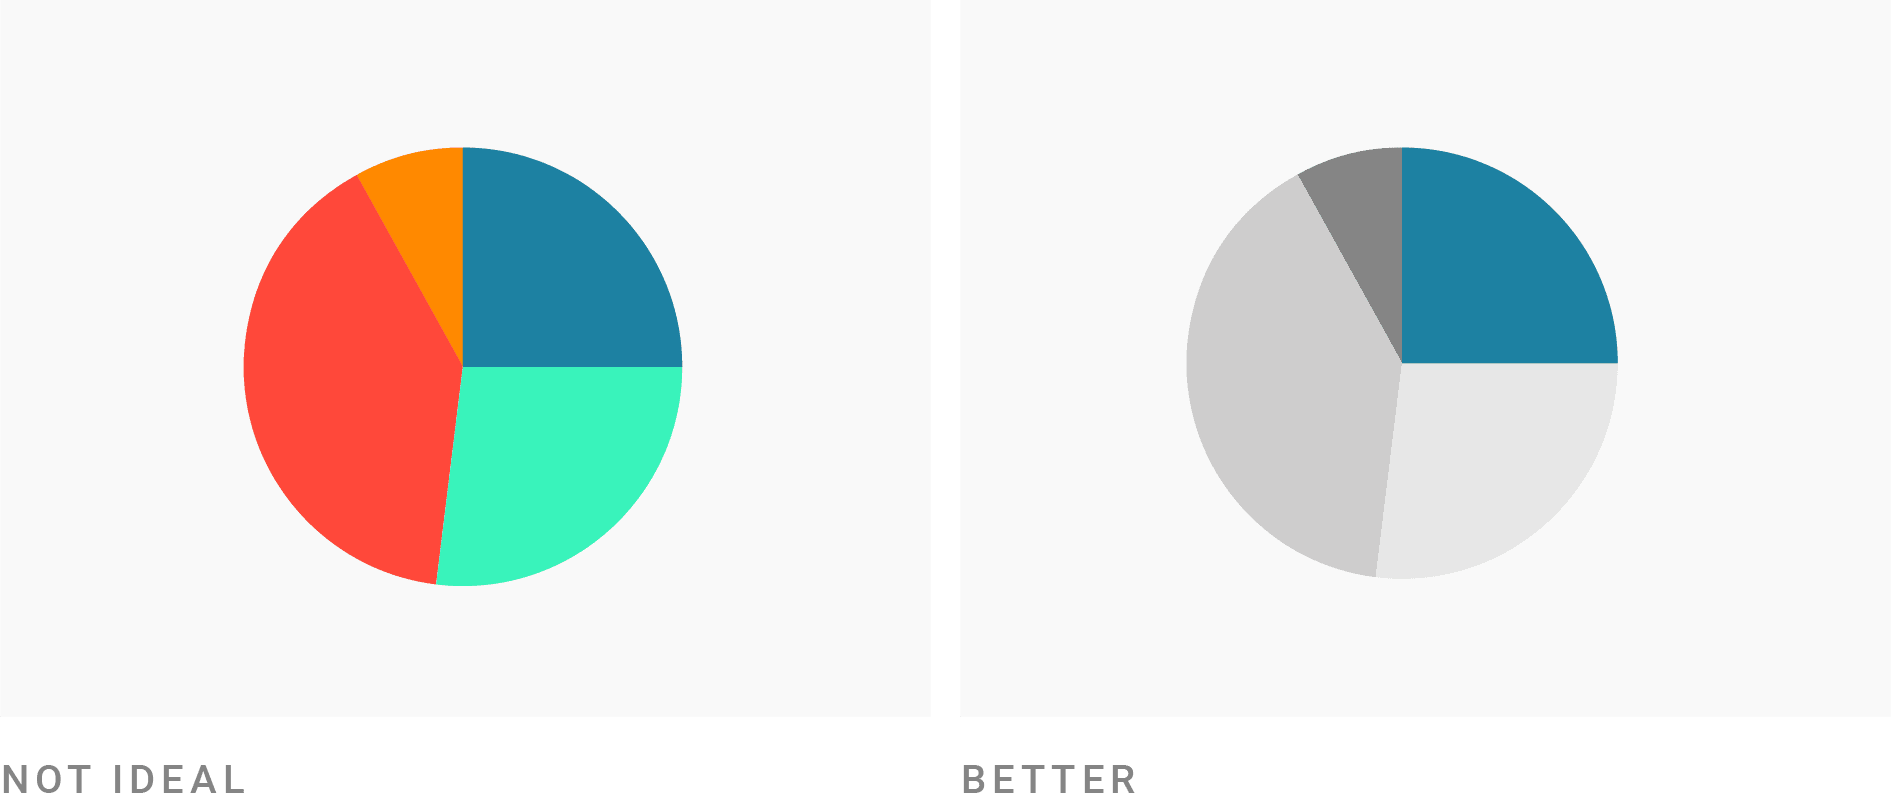
\includegraphics[width=\linewidth]{images/pie-chart/pie-chart-use-color-to-highlight.png}
        \fullwidthfigurecaption{Use one accent color for the key slice and quieter related hues for the rest; avoid rainbow palettes that make share comparison harder.}
        \label{fig:pie-chart-design-guidance-a}
        \label{fig:pie-chart-design-guidance-a-color-hierarchy}
    \end{minipage}
    \hfill
    \begin{minipage}[t]{0.48\linewidth}
        \centering
        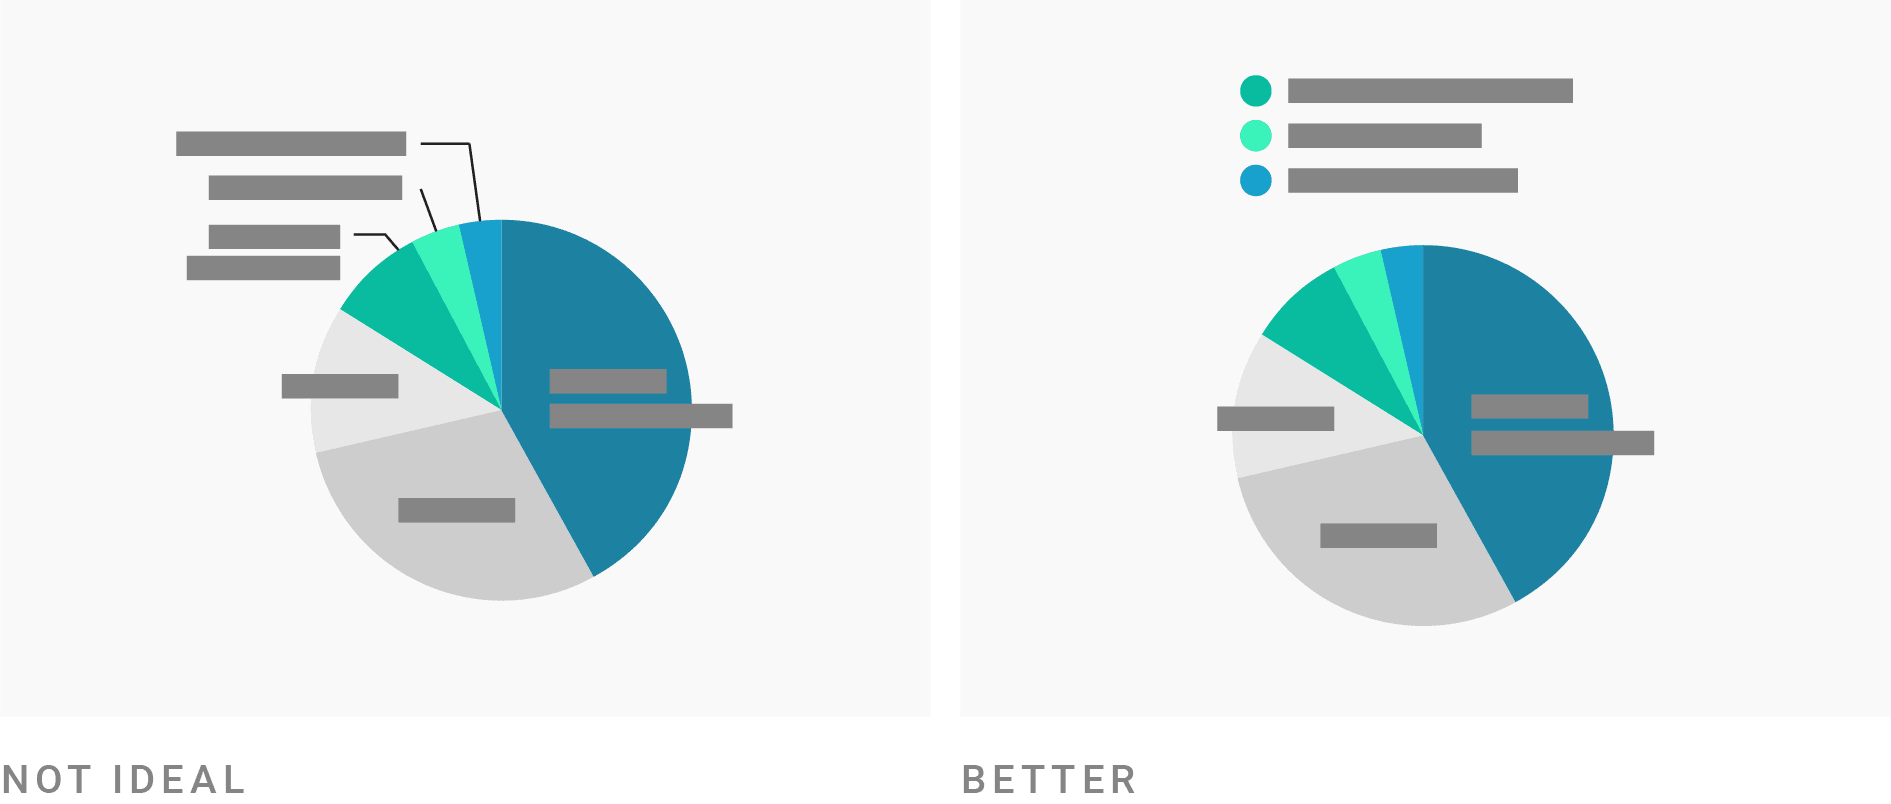
\includegraphics[width=\linewidth]{images/pie-chart/pie-chart-label-small-slices-outside.png}
        \fullwidthfigurecaption{Place labels outside when slices are small or text is long, then use leader lines if needed to keep category mapping unambiguous.}
        \label{fig:pie-chart-design-guidance-a-outside-labels}
    \end{minipage}
\end{figure*}

\begin{figure*}[htbp]
    \centering
    \begin{minipage}[t]{0.48\linewidth}
        \centering
        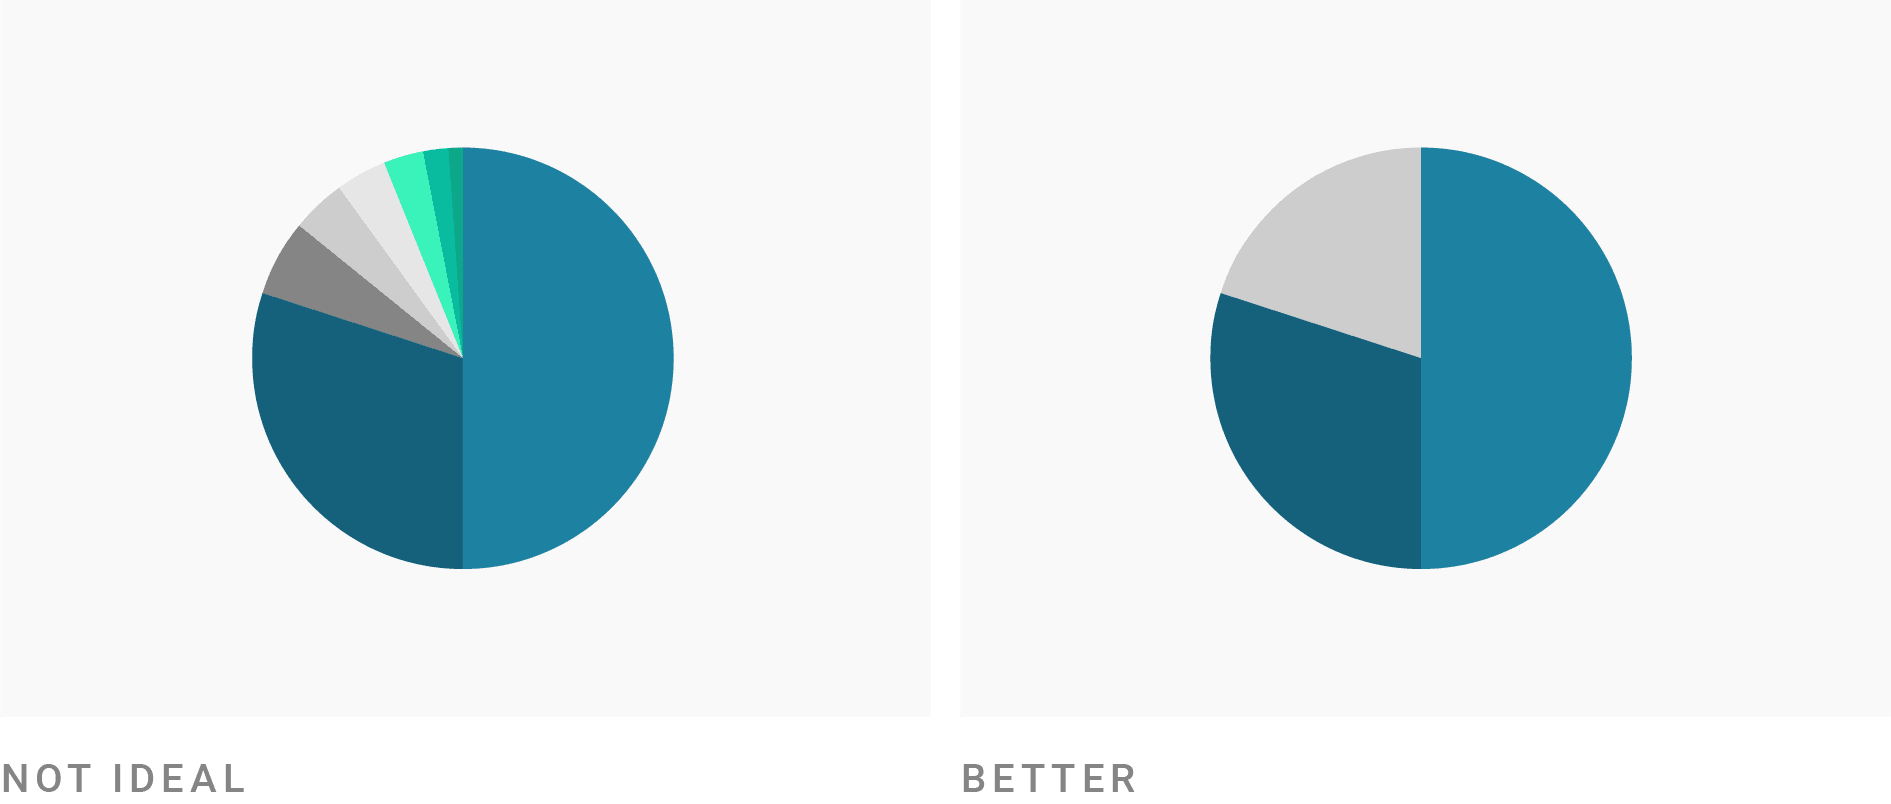
\includegraphics[width=\linewidth]{images/pie-chart/pie-chart-group-small-slices-others.png}
        \fullwidthfigurecaption{Group very small slices into ``Others'' so sectors are readable and the chart avoids excessive label clutter.}
        \label{fig:pie-chart-design-guidance-b}
        \label{fig:pie-chart-design-guidance-b-group-others}
    \end{minipage}
    \hfill
    \begin{minipage}[t]{0.48\linewidth}
        \centering
        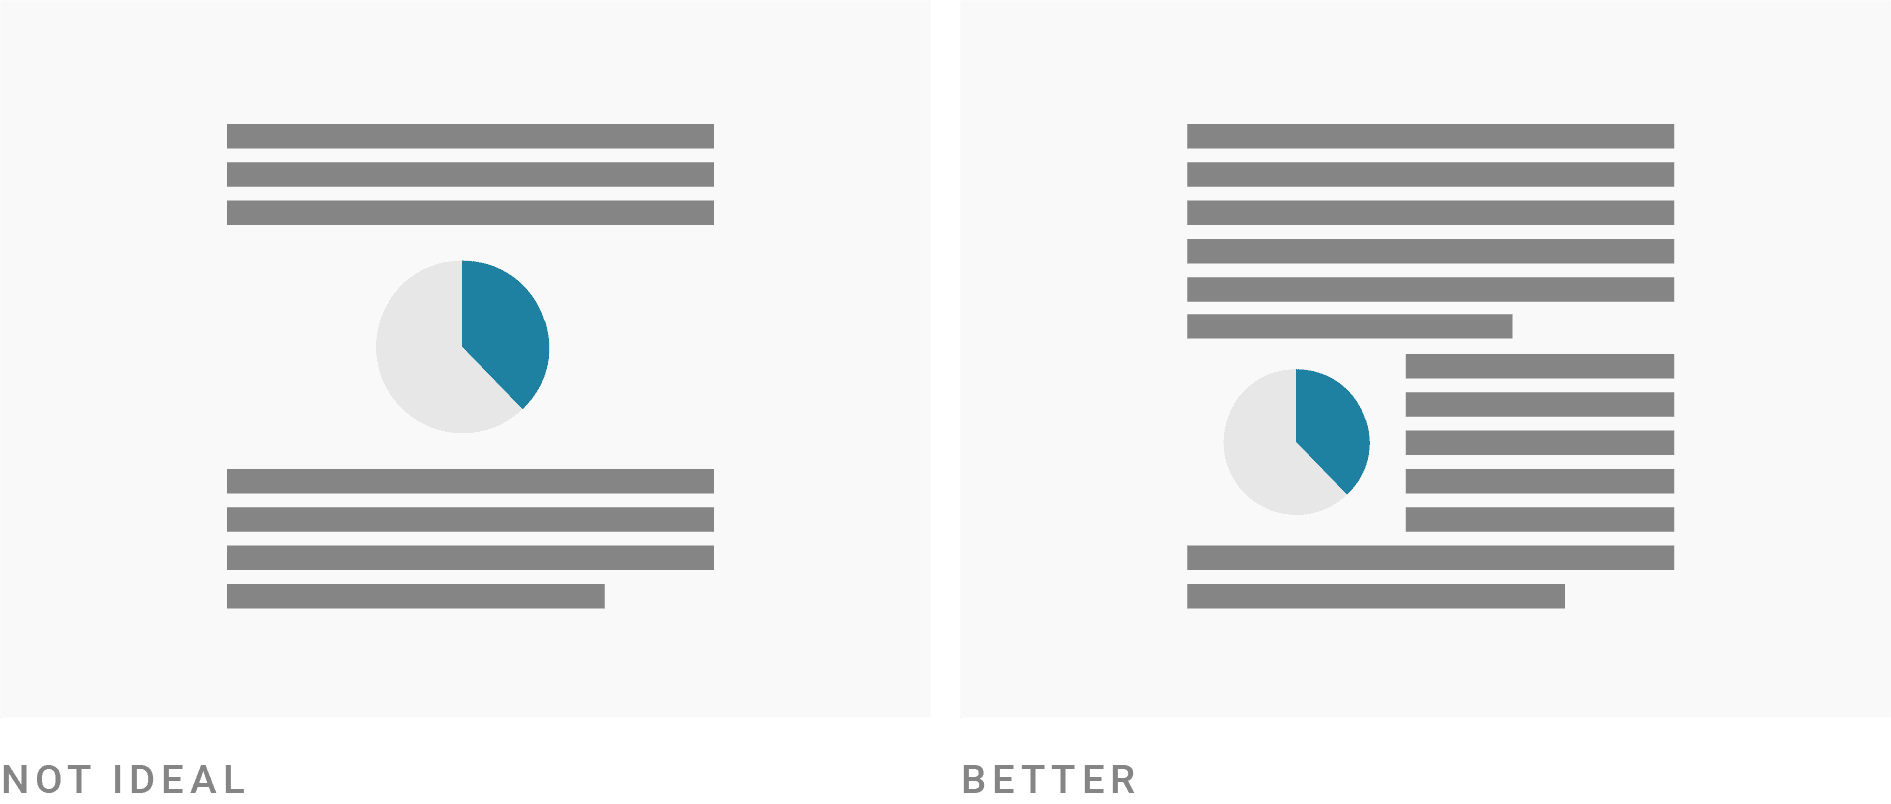
\includegraphics[width=\linewidth]{images/pie-chart/pie-chart-margin-or-sidebar-placement.png}
        \fullwidthfigurecaption{Use margin or sidebar placement for pies in text-heavy pages because fixed circular geometry often wastes space at full text width.}
        \label{fig:pie-chart-design-guidance-b-margin-placement}
    \end{minipage}
\end{figure*}

\subsection{Idiom: Scatterplots}
\paragraph{Brief}
A scatterplot maps each table record to one point in a Cartesian coordinate system. It is the core idiom for reading relationships between quantitative variables.

\whatpill\  A scatterplot uses two \textbf{quantitative value attributes} per \textbf{item}, mapped to x and y. Optional grouping adds one \textbf{categorical key attribute}.

\begin{figure*}[htbp]
    \centering
    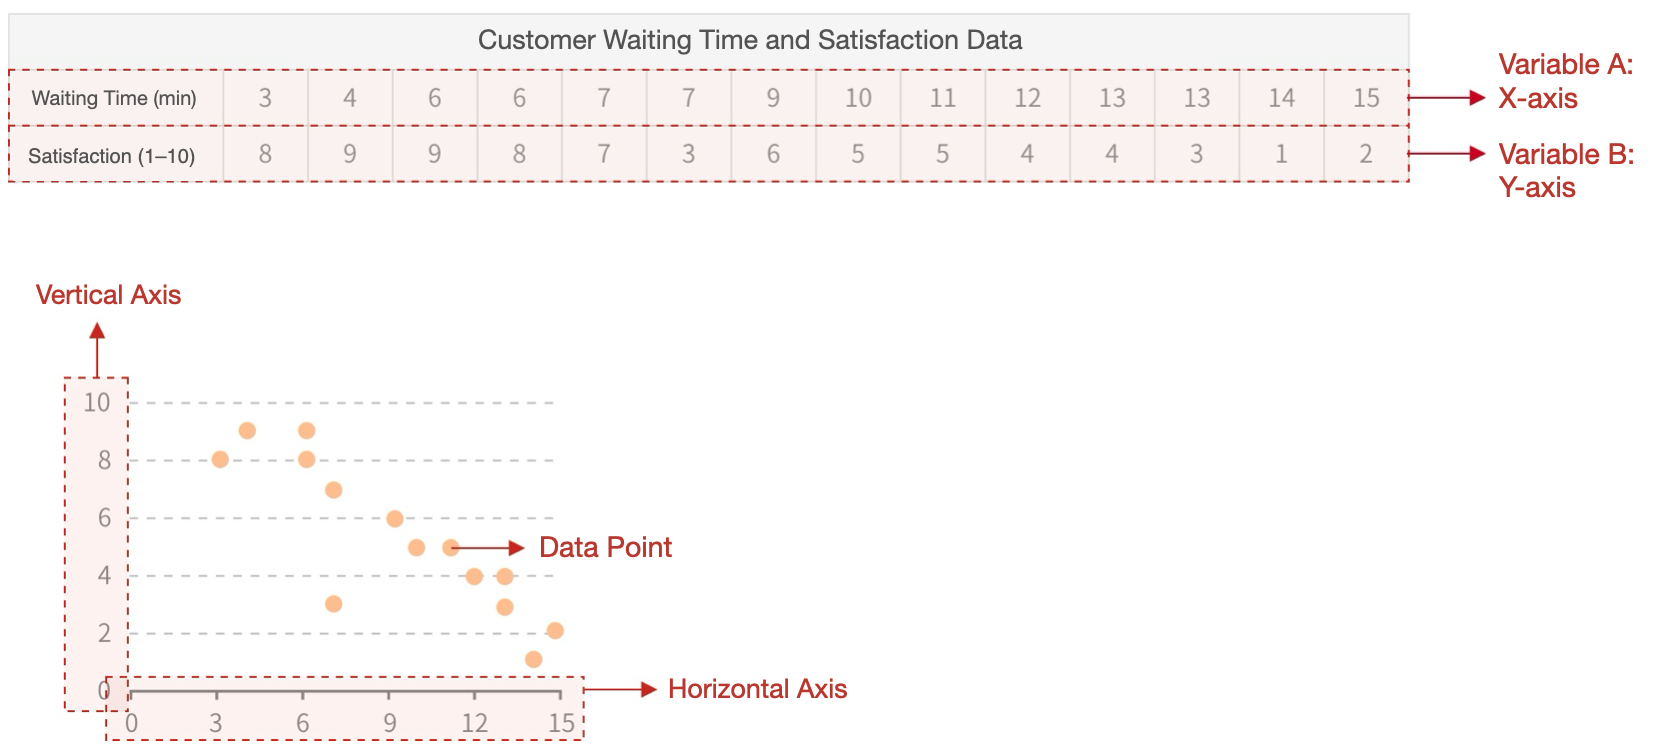
\includegraphics[width=0.92\linewidth]{images/scatter-plot/scatter-plot-elemental-composition.png}
    \caption{Elemental composition of a scatterplot: each record maps to one x/y point.}
    \label{fig:scatter-plot-elemental-composition}
\end{figure*}

\whypill\  The main \textit{task} is \textbf{analyse}, and the primary \textit{targets} are relationship form and distribution. Secondary \textit{actions} are \textbf{search} (outliers/clusters) and \textbf{query} (pairwise value comparison).

\howpill\  At the \textbf{idiom} level, the \textit{mark} is \textbf{point}. The dominant \textit{channels} are \textbf{horizontal position} and \textbf{vertical position}, with optional \textbf{hue} for categorical grouping. \textbf{Scalability} is typically to hundreds of items before overplotting controls are needed.





\subsection*{Design Guide}
\paragraph{Use when}
\begin{itemize}
    \item \textit{Correlation pattern detection.} Scatterplots are appropriate when we need to judge whether two variables are positively correlated, negatively correlated, nonlinear, or uncorrelated (see Figure~\ref{fig:scatter-plot-applicable-correlation}).
\begin{marginfigure}
    \centering
    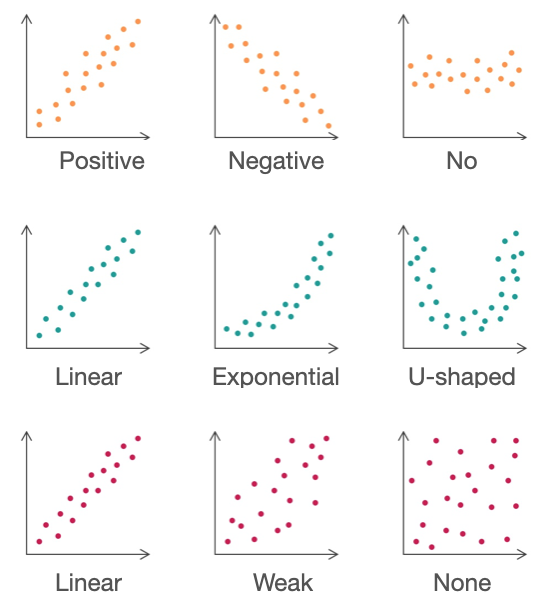
\includegraphics[width=1\linewidth]{images/scatter-plot/scatter-plot-applicable-correlation.png}
    \caption{Applicable usage: identify relationship forms, relative correlation strength, clusters, and outliers; treat visible correlation as association, not causal proof.}
    \label{fig:scatter-plot-applicable-correlation}
\end{marginfigure}

\begin{figure}[htp]
    \centering
    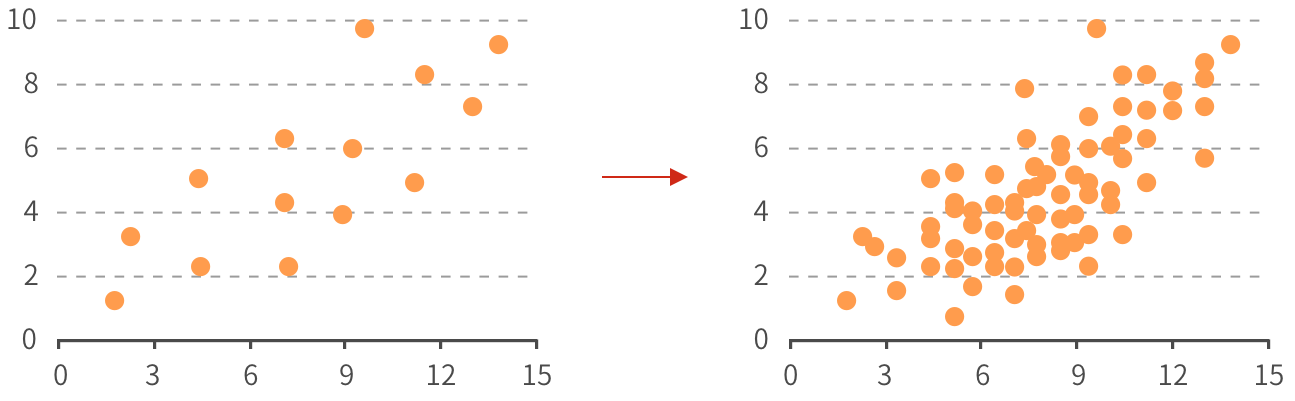
\includegraphics[width=1\linewidth]{images/scatter-plot/scatter-plot-applicable-many-points.png}
    \caption{Applicable usage: compare many records in a single quantitative relationship view so overall structure and relative groups become visible.}
    \label{fig:scatter-plot-applicable-many-points}
\end{figure}
    \item \textit{Large point-set comparison (non-temporal).} When we need to compare many records at once and read overall structure, scatterplots often become more informative as point count increases (see Figure~\ref{fig:scatter-plot-applicable-many-points}).
\end{itemize}


\paragraph{Avoid when}
\begin{itemize}
    \begin{marginfigure}
    \centering
    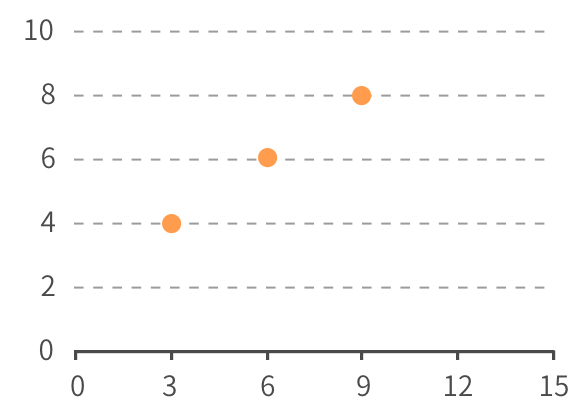
\includegraphics[width=0.92\linewidth]{images/scatter-plot/scatter-plot-inapplicable-too-few-points.png}
    \caption{Inapplicable usage: too few points for robust pattern judgement.}
    \label{fig:scatter-plot-inapplicable-too-few-points}
\end{marginfigure}

    \item \textit{Too few points.} Very small samples can make apparent patterns highly unstable and random (see Figure~\ref{fig:scatter-plot-inapplicable-too-few-points}).
    \begin{marginfigure}
    \centering
    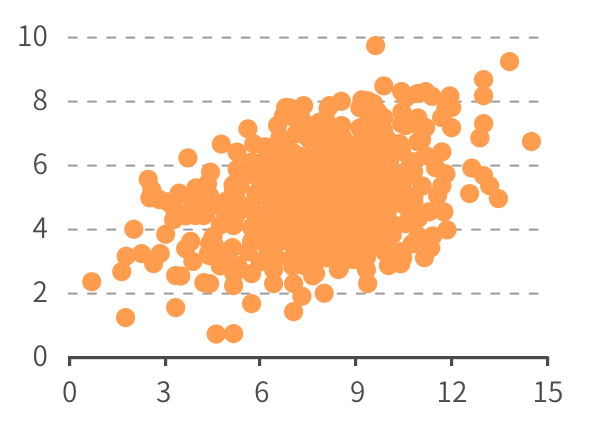
\includegraphics[width=\linewidth]{images/scatter-plot/scatter-plot-inapplicable-overplotting.png}
    \caption{Inapplicable usage: severe overplotting can hide structure; use transparency, smaller marks, sampling, aggregation (for example, hexbin), or filtering to recover legibility.}
    \label{fig:scatter-plot-inapplicable-overplotting}
    \label{fig:scatter-plot-inapplicable-overplotting-and-categories}
\end{marginfigure}
    \item \textit{Heavy overplotting.} If points are too dense or too large, mark overlap can hide structure. Common remedies include transparency, smaller points, sampling, grouping, density/hexbin alternatives, or interactive filtering (see Figure~\ref{fig:scatter-plot-inapplicable-overplotting-and-categories}).
    \begin{marginfigure}
    \centering
    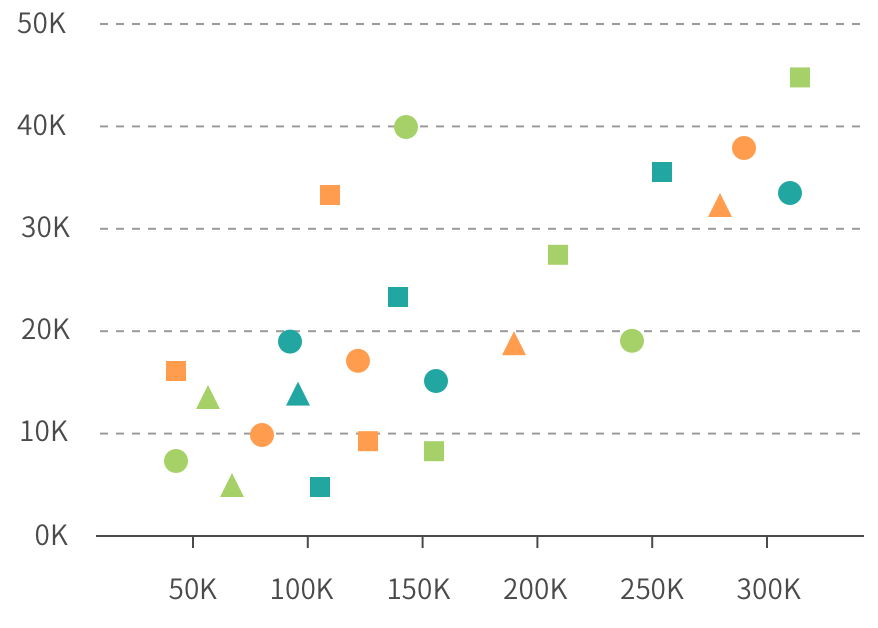
\includegraphics[width=\linewidth]{images/scatter-plot/scatter-plot-inapplicable-too-many-categories.png}
    \caption{Inapplicable usage: too many categories make quick discrimination difficult.}
    \label{fig:scatter-plot-inapplicable-too-many-categories}
\end{marginfigure}
    \item \textit{Correlation interpreted as causation.} A visible relationship in a scatterplot does not establish causality. External confounders can drive both variables.
\end{itemize}

%\paragraph{Wrap up}
%In summary, scatterplots are strong for relationship discovery, but interpretation quality depends on data density and analytical caution. Next, we will look at a multivariate extension of scatterplots: bubble plots.

\subsection*{Idiom: Bubble Plot}
\paragraph{Brief}
A bubble plot is a multivariate extension of the scatterplot. It keeps x/y position for two quantitative variables and adds bubble size for a third variable.

\whatpill\  A bubble plot keeps two \textbf{quantitative value attributes} for x/y and adds a third \textbf{quantitative value attribute} for bubble size; an optional \textbf{categorical key attribute} can be added for grouping.

\begin{figure}[htbp]
    \centering
    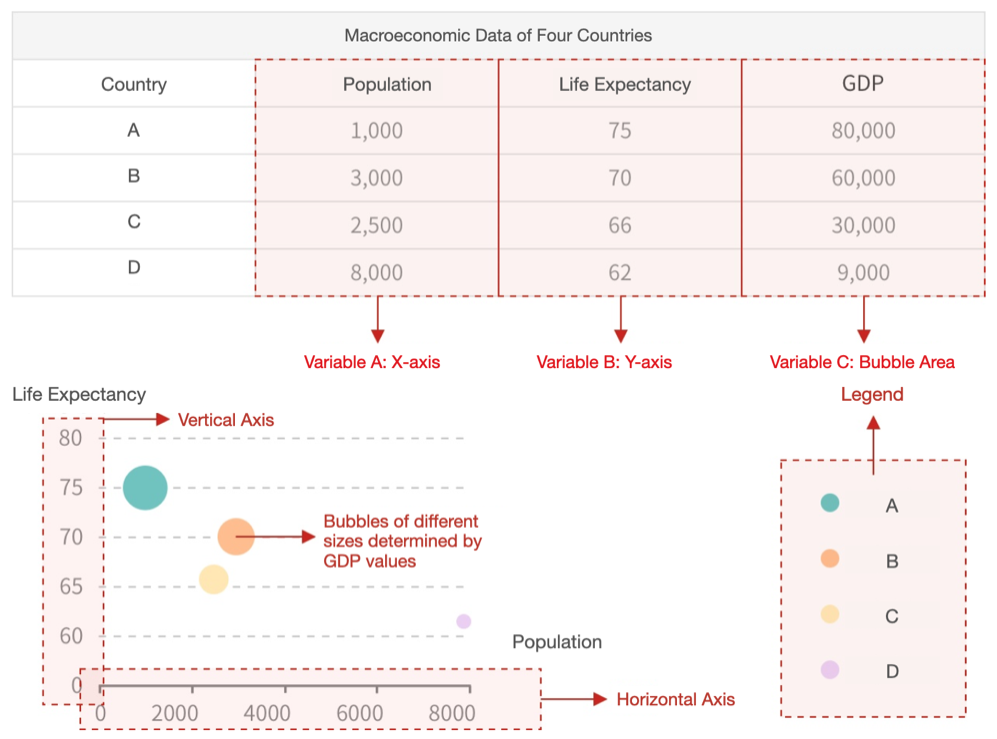
\includegraphics[width=\linewidth]{images/scatter-plot/bubble-plot-elemental-composition.png}
    \caption{Elemental composition of a bubble plot: x/y position plus bubble area for a third variable.}
    \label{fig:bubble-plot-elemental-composition}
\end{figure}

\whypill\  The main \textit{tasks} are \textbf{query} and \textbf{compare}, and the primary \textit{target} is three-variable \textbf{relationship} reading in one view. A secondary \textit{action} is \textbf{search} for size-related outliers or clusters when the size variable is substantively important.

\howpill\  At the \textbf{idiom} level, the \textit{mark} is \textbf{point}, with \textbf{area} variation for the third quantitative value. The primary \textit{channels} are position (x/y) plus area size; optional \textbf{hue} can encode a categorical key. For \textbf{expressiveness}, size must be scaled by area (not radius).

\subsection*{Design Guide}
\paragraph{Use when}
\begin{itemize}
    \item \textit{Compact multivariate comparison.} Use bubble plots when three quantitative variables must be compared in one static view, and size differences are an important part of the message (see Figure~\ref{fig:bubble-plot-warning}).
\end{itemize}

\begin{marginfigure}
    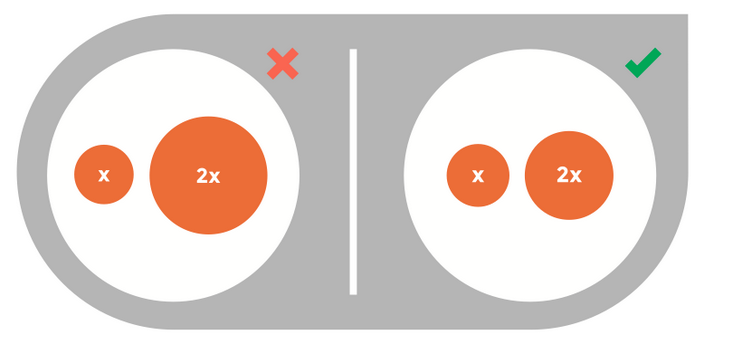
\includegraphics[width=\linewidth]{images/scatter-plot/bubble-plot-area-not-radius-warning.png}
    \caption{Bubble-plot usage: encode the third variable by bubble area (not radius), and use this idiom only when that third quantitative dimension is essential.}
    \label{fig:bubble-plot-warning}
\end{marginfigure}

\paragraph{Avoid when}
\begin{itemize}
    \item \textit{Dense bubbles in static views.} When bubble count and dimensions are too many, static views become cluttered. Interaction (hover/filter/search) is often needed to preserve readability.
\end{itemize}

% \begin{marginfigure}
%     \centering
%     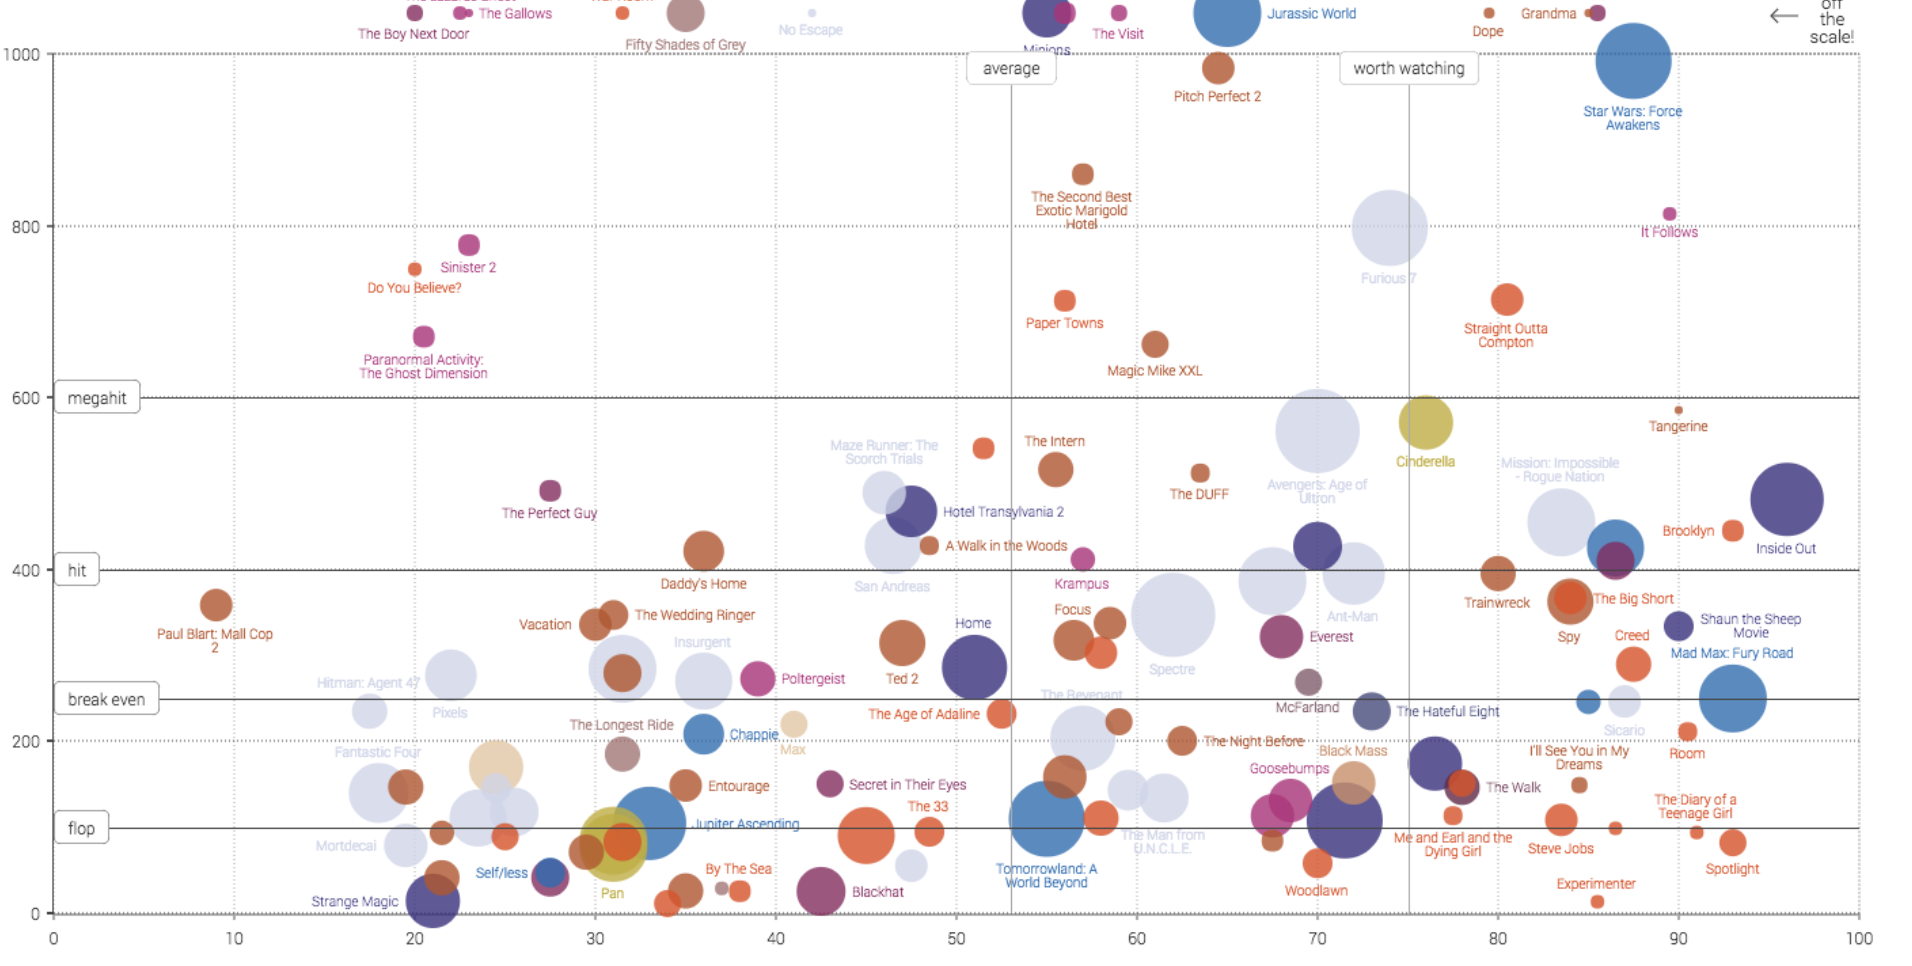
\includegraphics[width=\linewidth]{images/scatter-plot/bubble-plot-inapplicable-too-many-bubbles-no-interaction.png}
%     \caption{Bubble-plot limitation: dense multi-category bubbles usually require interaction or simplification to avoid unreadable overlap.}
%     \label{fig:bubble-plot-inapplicable-too-many}
% \end{marginfigure}

%\paragraph{Wrap up}
%In summary, bubble plots can encode a third quantitative variable effectively, but only when size scaling and density control are handled carefully. The key refinement suggestions are: see Figure~\ref{fig:bubble-plot-warning}.

\section{Summary Snapshot}
\begin{table*}[htbp]
    \centering
    \footnotesize
    \begin{tabular}{@{}p{0.17\linewidth}p{0.26\linewidth}p{0.24\linewidth}p{0.25\linewidth}@{}}
        \textbf{Idiom} & \textbf{What} & \textbf{Why} & \textbf{How} \\
        \hline
        Bar chart & 1 categorical + 1 quantitative & Compare, rank, lookup & Aligned bar length, shared baseline \\
        Line chart & 1 ordered + 1 quantitative & Trend and peaks & Position with line connection \\
        Area chart & Category + time + quantitative & Trend with accumulation & Filled area height + hue \\
        Pie chart & 1 categorical + 1 quantitative & Part-to-whole & Angle/area proportion \\
        Dot plot & Item + quantitative (single/multiple) & Comparison and change & Point position, optional connectors \\
        Scatterplot & 2 quantitative (or more via SPLOM) & Correlation, clusters, outliers & x/y position, optional hue/size \\
    \end{tabular}
    \caption{Summary idiom map using the What--Why--How lens.}
    \label{tab:idiom-selection-snapshot}
\end{table*}
